\documentclass[a4paper,12 pt,titlepage,twoside]{book}
\usepackage[T1]{fontenc}
\usepackage{lmodern}
\usepackage[utf8]{inputenc}
\usepackage[british]{babel}
\usepackage[margin=3cm]{geometry}
\geometry{a4paper,top=3cm,bottom=3cm,left=3.5cm,right=3.5cm,heightrounded,bindingoffset=5mm}
\usepackage{color}
\usepackage{amsthm}
\usepackage{amsmath,amssymb}
\usepackage{graphicx}
\usepackage{mathtools}
\usepackage{listings}
\usepackage{newlfont}
\usepackage[all,cmtip]{xy}
%\usepackage{tikz}
\usepackage{tikz,fullpage}
\usetikzlibrary{arrows,%
	petri,%
	topaths}%
\usepackage{tkz-berge}
%\usepackage[position=top]{subfig}
\usepackage{tikz-cd}
\usepackage{rotating}
\usepackage{rotating}
\usepackage{marvosym}
\usepackage{extarrows}
\usepackage{enumitem}
\usepackage{subcaption}
\usepackage{booktabs}
\usepackage{MnSymbol}
\usepackage{emptypage}
%\usepackage{newlfont}
%\usepackage[pdfborder={0 0 0.6}]{hyperref}
%\usepackage{apacite}


\newcommand{\numberset}{\mathbb}
\newcommand{\N}{\numberset{N}}
\newcommand{\Z}{\numberset{Z}}
\newcommand{\R}{\numberset{R}}
\newcommand{\Q}{\numberset{Q}}
\newcommand{\K}{\numberset{K}}
\newcommand{\F}{\numberset{F}}
\newcommand{\C}{\numberset{C}}
\newcommand{\n}{\mathcal{N}}
\newcommand{\aid}{\mathfrak{a}}
\newcommand{\bid}{\mathfrak{b}}
\newcommand{\pid}{\mathfrak{p}}
\newcommand{\qid}{\mathfrak{q}}
\newcommand{\mi}{\mathfrak{m}}
\newcommand{\I}{\mathbb{I}}
\newcommand{\V}{\mathbb{V}}
\newcommand{\A}{\mathbb{A}}
\newcommand{\Ps}{\mathbb{P}}
\newcommand{\os}{\mathcal{O}}
\newcommand{\exercise}[1]{\noindent {\bf Exercise #1}}
\newcommand{\solution}[1]{\noindent {\bf Solution #1}}
\newcommand*{\isoarrow}[1]{\arrow[#1,"\rotatebox{90}{\(\sim\)}"]}
\newcommand\dhrightarrow{%
	\mathrel{\ooalign{$\rightarrow$\cr%
			$\mkern3.5mu\rightarrow$}}
}

\newcommand\dhxrightarrow[2][]{%
	\mathrel{\ooalign{$\xrightarrow[#1\mkern4mu]{#2\mkern4mu}$\cr%
			\hidewidth$\rightarrow\mkern4mu$}}
}
\newcommand\mapsfrom{\mathrel{\reflectbox{\ensuremath{\mapsto}}}}
\newcommand{\set}{\underline{Set}}
\newcommand{\epsi}{\varepsilon}
\newcommand{\Lie}{\mathcal{L}ie}
\newcommand{\ls}{\mathcal{L}}


\DeclareMathOperator{\Ima}{Im}
\DeclareMathOperator{\Op}{Open}
\DeclareMathOperator{\coker}{coker}
\DeclareMathOperator{\Id}{Id}
\DeclareMathOperator{\map}{Map}
\DeclareMathOperator{\rk}{rk}
\DeclareMathOperator{\ch}{char}
\DeclareMathOperator{\di}{div}
\DeclareMathOperator{\spec}{Spec}
\DeclareMathOperator{\het}{ht}
\DeclareMathOperator{\trdeg}{Trdeg}
\DeclareMathOperator{\mcg}{MCG}
\DeclareMathOperator{\Hom}{Hom}
\DeclareMathOperator{\home}{Homeo}
\DeclareMathOperator{\id}{id}
\DeclareMathOperator{\bl}{Bl}
\DeclareMathOperator{\pic}{Pic}
\DeclareMathOperator{\pico}{Pic^0}
\DeclareMathOperator{\cl}{Cl}
\DeclareMathOperator{\an}{an}
\DeclareMathOperator{\Span}{Span}
\DeclareMathOperator{\res}{Res}
\DeclareMathOperator{\lie}{Lie}
\DeclareMathOperator{\sing}{sing}
\DeclareMathOperator{\IH}{IH}
\DeclareMathOperator{\br}{Br}

\theoremstyle{plain}
\newtheorem{thm}{Theorem}[section]

\theoremstyle{theorem}
\newtheorem{fact}[thm]{\textbf{Fact}}
\newtheorem{lemma}[thm]{Lemma}
\newtheorem{prop}[thm]{Proposition}
\newtheorem{cor}[thm]{Corollary}

\theoremstyle{definition}
\newtheorem{defn}[thm]{Definition}
\newtheorem{exm}[thm]{Example}


\theoremstyle{remark} 
\newtheorem{oss}[thm]{Remark} 
\newtheorem{claim}{Claim}
\newtheorem*{claim*}{Claim}





\begin{document}
	\thispagestyle{empty}
	\begin{titlepage}
		\begin{center}
			\begin{figure}[h!]
				\centering
				\includegraphics[width=0.3\linewidth]{Logo_Algant}
				%\includegraphics{algant_logo}
			\end{figure}
			\vspace{0.4cm}
			\fontsize{15pt}{0.6cm}\selectfont
			{\textbf{ALGANT Master Thesis}}
			\vspace{0.2cm}
			\rule{\linewidth}{0.3mm}
			
			\vspace{0.05cm}
			\Huge{\textbf{Asymptotic height pairing 
					\\ %\vspace{.25em} 
					for families of curves\\ with stable degeneration}}\\
			\vspace{0.05cm}
			
			\rule{\linewidth}{0.3mm}
			
			\vspace{0.1cm}
			
			\large{\textbf{Fabio Buccoliero}}\\
			\vspace{0.1cm}
			
			\large{\textbf{Supervisor: dr.\ R.S.\ de Jong}}
			
			\vfill
			
			\begin{figure}[h!]
				\centering
				\begin{minipage}{0.5\linewidth}
					\centering
					\includegraphics[width=1.1\linewidth]{Logo_Milano}
				%	\includegraphics[width=0.60\textwidth]{milan_logo}
				\end{minipage}\hfill
				\begin{minipage}{0.5\linewidth}
					\centering
				%	\includegraphics[width=0.60\textwidth]{ulzegel_blauw}
					\includegraphics[width=0.9\linewidth]{Logo_Leiden}
				\end{minipage}
			\end{figure}
			\rule{\linewidth}{0.2mm}\\
			\small{Academic Year 2019-2020}
		\end{center}
	\end{titlepage}
%	\vspace*{1em}
%	\begin{center}
%		\includegraphics{algant_logo}
%		\vspace{3em}	
%		{\Large\bf 
%			Fabio\ Buccoliero
%		} 	
%		\vspace{1em} 	
%		{\LARGE\bf 
%			Asymptotic height pairing 
%			\\ \vspace{.25em} 
%			for families of curves with stable degeneration
%		} 
%		\vspace{6em} 
%		{\large\bf 
%			ALGANT Master Thesis
%		} 
%		\vspace{1em}
%		{\large\bf 
%			15 July 2020
%		}	
%		\vspace{6em} 
%		{\large\bf
%			\begin{tabular}{ll}
%				Thesis supervisor: & prof.dr.\ R.S.\ de Jong\\
%			\end{tabular}
%		}
%		\vfill
%		\includegraphics[width= 0.2\textwidth]{milan_logo} \hfill \includegraphics{ulzegel_blauw}\\
%		\vspace{2em}
%		{\large\bf
%			Università degli Studi di Milano
%		}	\hfill	{\large\bf 
%			%\begin{tabular}{ll}
%			Universiteit Leiden\\
			%& Mathematical Institute\\
			%\end{tabular}
%		}		
%	\end{center}
	
	
	
%\setcounter{section}{-1}
\chapter*{Introduction}
\addcontentsline{toc}{chapter}{Introduction}
	The inspiration for this thesis comes from a paper by Brosnan and Pearlstein (\cite{MR3983292}), where the authors introduce the asymptotic height pairing in a general context. In particular, they find out that the asymptotic height pairing computes the \emph{height jump}, a notion introduced by Hain in \cite{MR2059020}. The height jump has already been computed, in the case of families of degree zero divisors, by Holmes and de Jong in \cite{MR3488379}, using the N{é}ron height pairing. Therefore, the final goal of this thesis is to understand if, in the setting studied in \cite{MR3488379}, the height jump computed via the asymptotic height pairing coincides with the height jump computed via the N{é}ron height pairing.
	
	In this thesis, we study the asymptotic height pairing of the singularities of admissible normal functions coming from families of degree-zero divisors on a family of curves with stable degeneration. In this special setting, it is possible to associate a graph to the central fiber of the family. It is well-known that several properties of the family can actually be obtained from the graph.
	
	The first goal of this thesis is to show that one of the properties that one can recover studying the graph is exactly the asymptotic height pairing of the family. More precisely, we consider a $n$-pointed family of curves with stable degeneration $(f \colon X \rightarrow \Delta^r, (x_1, \dots, x_n))$ over the polydisk. We denote its central fiber with $X_0$ and we let $\Gamma$ be its dual graph. We consider two families of divisors of degree zero, $D_\alpha, D_\beta$, and we associate admissible normal functions, $\nu_\alpha, \nu_\beta,$ with them. The singularities of these normal functions can be computed by the asymptotic height pairing. In Theorem \ref{explicit formula} we derive a new explicit formula to compute the asymptotic height pairing of $\sing(\nu_\alpha), \sing(\nu_\beta)$. The peculiarity of this formula is that it involves solely information coming from $\sing(\nu_\alpha), \sing(\nu_\beta)$ and the dual graph $\Gamma$ associated to the central fiber of the family. In particular, it makes the formula of Proposition 126 of \cite{MR3983292} more explicit and more easily computable, because it gets rid of the term $l(t)$ defined via Proposition 120.
	
	The second goal of this thesis was the one already discussed at the beginning of this introduction. In particular it derives from both Theorem 252 of \cite{MR3983292} and the proof of Theorem 2.4 of \cite{MR3488379}. In these results, the authors showed that, respectively, the asymptotic height pairing and the Green's function computed the height jump. Thanks to the new formula obtained in Theorem \ref{explicit formula} and to some computations on the total contraction $\overline{\Gamma}$ of the dual graph $\Gamma$, we prove, in Theorem \ref{thm: equality green ahp}, that these two results actually match. Without using the height jump, but only using graph-related results, we manage to prove that the asymptotic height pairing of $\sing(\nu_\alpha),\sing(\nu_\beta)$ is equal to the Green's function of $\overline{D_\alpha}, \overline{D_\beta}$, the projections of $D_\alpha, D_\beta$ on the total contraction $\overline{\Gamma}$ of the graph $\Gamma$.
	
	In the first two chapters, we introduce the machinery that we need later on in the thesis. The main references for these introductory sections are chapters 10 and 11 of \cite{MR2807457}.
	In particular, in chapter \ref{sec: picard-lefschetz theory} we introduce some notions of the Picard-Lefschetz theory, such as the mapping class group of a surface (\cite{massuyea2009short}, \cite{wilton_2019}), the equivalence of categories between local systems and representations of the fundamental group (\cite{MR3025862}, \cite{achar_2007}), the Picard-Lefschetz representation and the universal deformation space (\cite{MR2807457}).
	In chapter \ref{sec: dual graph and homology} we introduce the dual graph associated to a nodal curve $C$ and we investigate interesting properties which link this graph to the universal deformation of $C$ (\cite{MR2807457}).
	
	In chapter \ref{sec: classification of stable curves genus 2} we classify the stable curves of genus 2 by studying their dual graph. This section is an example of the reason why we deal with stable curves and how powerful the dual graph is when we consider this kind of curves. In chapter \ref{monodromy pairing}, we follow section 3 of \cite{MR3588803} to introduce the monodromy pairing on a family of curves with stable degeneration. The authors show in \cite{MR3588803} that this pairing is the same as the cycle pairing defined on the cohomology of the dual graph of the family. This equality will play an important role in the proof of Theorem \ref{explicit formula}. In chapter \ref{sec: ahp} we define the asymptotic height pairing in a general context as is done by Brosnan and Pearlstein in section 6 of \cite{MR3983292}. In chapter \ref{sec: singularities of normal functions} we introduce the Griffiths intermediate jacobian (\cite{MR3184171}) associated to a family of smooth projective complex varieties and we define the admissible normal function associated to a family of cycles. We give also a cohomological interpretation of the singularity of such admissible normal functions, which will play a role in Theorem \ref{explicit formula}.
	
	The last two chapters contain some results of our own. In fact, chapter \ref{sec: an explicit formula for the ahp} is completely devoted to the statement and the proof of Theorem \ref{explicit formula}. In chapter \ref{sec: the ahp coincides with green} we first introduce the Green's function and the contraction of a graph (\cite{MR3488379}, \cite{MR2794031}), then we state Theorem \ref{thm: equality green ahp} and prove it. In the conclusion, we make some remarks about how this result links together both \cite{MR3983292} and \cite{MR3488379}.
	\newpage
\chapter*{Acknowledgements}
I would like to thank my supervisor, dr. Robin de Jong, both for suggesting me this intriguing topic and for helping and guiding me in every step of the creation of this thesis.

Thank you to dr. M{à}rton Hablicsek and to dr. David Holmes for reading and correcting the thesis. 

Thank you to dr. David Holmes and to prof. Bas Edixhoven for the interesting questions and comments, which helped me to better understand the topic I was studying.

I would like to thank all the professors and the staff in Leiden and in Milan universities and all the ALGANT consortium to make this experience possible. 

Thank you to my girlfriend and to all the friends I met in Milan and in Leiden. A special thank you goes to Margherita, who not only as a friend but also as a roommate has shared her time and advice with me.\\

Grazie a coloro senza cui questo viaggio non sarebbe nemmeno mai iniziato: i miei genitori. Grazie per il sostegno morale, fisico, psicologico ed economico. Non credo che riuscirò mai a trasmettervi davvero quanto vi sia grato per avermi permesso di intraprendere questa strada e per esserci sempre stati. Grazie a tutta la mia famiglia. Grazie ai miei amici, che hanno sempre continuato a credere in me.\\
\begin{flushright}
	Fabio Buccoliero \\ Leiden, June 2020
\end{flushright}
\newpage
	
\tableofcontents
\newpage
	
\chapter{Some concepts of Picard-Lefschetz theory}\label{sec: picard-lefschetz theory}
We start with some preliminaries about Picard-Lefschetz theory that we will consistently use throughout the thesis. The first three sections are devoted to construct the setting in which we will work for the whole thesis. In particular, we define the Picard-Lefschetz representation (\ref{sec: picard-lefschetz transformations}) and the universal deformation space of a \emph{stable} curve (\ref{sec: uni def space}).
\section{The mapping class group}
In this section, we introduce the mapping class group of a surface. This object will be fundamental in section \ref{sec: picard-lefschetz transformations} to talk about the Picard-Lefschetz representation. Moreover, we also talk about \emph{Dehn twists}, which generate the mapping class group. In this section we will follow mainly section 10.9 of \cite{MR2807457} and sections 1, 2, and 5 of \cite{massuyea2009short}.
\subsection{Definition}
Consider a compact connected orientable surface $\Sigma$ of genus $g$. We denote it with $\Sigma_g$ when we want to keep track of its genus. 

We give an orientation to $\Sigma$ and we define its mapping class group in the following way.
\begin{defn}
	The \emph{mapping class group} of $\Sigma$ is the group $$\mcg(\Sigma) := \home^+(\Sigma)/\sim$$ of orientation-preserving homeomorphisms $f \colon \Sigma \rightarrow \Sigma$ up to isotopy.
\end{defn}
Another interesting situation that we will consider in this thesis is the case of a  \emph{marked surface} $\Sigma$, i.e. when $n$ distinct points are chosen on the surface $\Sigma$.
\begin{defn}
	Let $\Sigma$ be a surface and let $p_1, \dots, p_n$ be $n$ distinct points on $\Sigma.$ The \emph{mapping class group of $\Sigma$ relative to $(p_1,\dots,p_n)$} is the subgroup of the mapping class group of $\Sigma$ $$\mcg(\Sigma, (p_1, \dots, p_n)) \subseteq \mcg(\Sigma),$$ where we consider only orientation-preserving homeomorphisms which fix $(p_1,\dots,p_n).$ 
\end{defn}
\begin{oss}\label{rmk: functoriality of mcg}
	Notice that, by functoriality, we have a natural map from the mapping class group of a surface $\Sigma$ towards the automorphisms of its first singular homology group: $$\rho \colon \mcg(\Sigma) \rightarrow \text{Aut}(H_1(\Sigma,\Z)) = \text{GL}(H_1(\Sigma, \Z)).$$
\end{oss}
Before presenting an example of how to compute the mapping class group of the torus, we need first to introduce the \emph{intersection pairing}.

\subsection{The intersection pairing}
Let $\Sigma_g$ be a compact connected orientable surface of genus $g$. $\Sigma_g$ can be identified as a torus of genus $g$. We know that its first homology group $H_1(\Sigma_g,\Z)$ is a free abelian group of rank $2g$. $H_1(\Sigma_g,\Z)$ is equipped with a symplectic form, namely the intersection pairing.
\begin{defn}\label{lem: intersection pairing}
	The \emph{intersection pairing} $$Q \colon H_1(\Sigma_g,\Z) \times H_1(\Sigma_g,\Z) \rightarrow \Z$$ is a symplectic form, i.e. a bilinear, alternating, non-degenerate form, on $H_1(\Sigma_g,\Z).$ Fixing a symplectic basis of $H_1(\Sigma_g, \Z)$, the intersection pairing is represented by the matrix $$Q := \left(\begin{array}{c|c}
	0 & I_g \\ \hline -I_g & 0\end{array}\right).$$
\end{defn}
\begin{exm}
	To understand better how the intersection pairing works, we introduce the \emph{geometric intersection number} of two simple closed curves on a compact connected orientable surface $\Sigma$ (we are not interested in highlightening its genus in this definition).
	\begin{defn}
		Given two simple closed curves $\alpha,\beta \subset \Sigma$ we define their \emph{geometric intersection number} as $$i(\alpha,\beta):= \min\{|\alpha' \cap \beta'| \in \N \mid \alpha' \text{ is isotopic to } \alpha, \beta' \text{ is isotopic to } \beta, \alpha' \text{ intersects transversally } \beta'\},$$ where by transversal intersection we mean the following: if we call $p \in \Sigma$ a point of intersection between $\alpha'$ and $\beta'$ and we consider the tangent vectors $v_{\alpha'}$ of $\alpha'$ at $p$ and $v_{\beta'}$ of $\beta'$ at $p$, then we want that their scalar product (defined in the tangent space at $p$ of $\Sigma$) vanishes: $$\langle v_{\alpha'}, v_{\beta'}\rangle =0.$$
	\end{defn}
	Informally, to compute the intersection pairing of two cycles $a,b \in H_1(\Sigma_g,\Z)$ \emph{up to sign}, one can first find representatives $\alpha,\beta$ of $a,b$ in $\Sigma_g$ and then compute their geometric intersection number. This gives an idea of which is the value of their intersection pairing.
\end{exm}
\begin{oss}\label{rmk: intersection pairing is perfect}
	From Lemma \ref{lem: intersection pairing}, one gets that the determinant of the intersection pairing is $$\det Q = \det \left(\begin{array}{c|c} 0 & I_g \\ \hline -I_g & 0
	\end{array}\right) = 1 \in \Z^\times.$$ Hence, we have that $Q$ is a unimodular matrix and this implies that the intersection pairing is a perfect pairing, i.e. it induces an isomorphism $$Q \colon H_1(\Sigma_g,\Z) \stackrel{\sim}{\longrightarrow} H_1(\Sigma_g,\Z)^\vee.$$
\end{oss}

As a useful example, we compute the mapping class group of a torus. This is an interesting method to compute the mapping class group of a surface, which uses its universal covering.

Consider the group homomorphism $$M \colon \mcg(S^1\times S^1) \rightarrow \text{GL}(2,\Z), \quad [f] \mapsto f_*,$$ where $f_*$ is the matrix of the map $f_* \colon H_1(S^1\times S^1,\Z) \rightarrow H_1(S^1\times S^1,\Z)$ relative to the basis $(a =[S^1 \times 1],b= [1 \times S^1])$ of $S^1\times S^1$.
\begin{prop}
	The map $M$ induces a group isomorphism between $$\mcg(S^1 \times S^1) \simeq \text{SL}(2,\Z).$$
\end{prop}
\begin{proof}
	First, we want to show that the image of $M$ is actually contained in $\text{SL}(2,\Z):$ take $[f] \in \mcg(S^1\times S^1),$ then we have that $$M([f]) = \left(\begin{array}{cc} Q(f_*(a),b) & Q(f_*(b),b)\\ Q(-f_*(a),a) & Q(-f_*(b),b)
	\end{array}\right),$$ where $Q$ denotes the intersection pairing. If we suppose that $f_*(a)=ma+nb$ and $ f_*(b)=ka+hb,$ the matrix $M([f])$ becomes $$M([f]) = \left(\begin{array}{cc} m & n \\ k & h \end{array}\right).$$ Being $f$ an orientation-preserving homeomorphism, it preserves the intersection pairing, i.e. for every $x,y \in H_1(S^1\times S^1,\Z)$ we have $$Q(f_*(x), f_*(y)) = Q(x,y).$$ Hence we get $$\det M([f]) = mh-nk = Q(f_*(a),f_*(b)) = Q(a,b) = 1,$$ because the intersection pairing is a symplectic form. Now, we want to show that $M$ is surjective onto $\text{SL}(2,\Z).$ Indeed, identify $S^1\times S^1$ with $\R^2/\Z^2,$ sending $a \mapsto [0,1]\times 0, b \mapsto 0 \times [0,1].$ Take $T \in \text{SL}(2,\Z), $ this defines a homeomorphism $\R^2 \rightarrow \R^2$ which factors through $\Z^2$, call $t \colon \R^2/\Z^2 \rightarrow \R^2/\Z^2$ the orientation-preserving homeomorphism induced. It is such that $t_* \colon H_1(S^1 \times S^1,\Z) \rightarrow H_1(S^1\times S^1,\Z)$ is represented by the same matrix as $T$. Thus, we have that $M([t]) = T.$ We are left to show the injectivity of $M$. Take $f \colon S^1 \times S^1 \rightarrow S^1\times S^1$ homeomorphism such that $M([f])$ is trivial, i.e. $f_*(a)=a, f_*(b)=b.$ We know that $\pi_1(S^1 \times S^1) = H_1(S^1 \times S^1,\Z)$ as it is abelian, so we have that $f_*$ acts trivially on $\pi_1(S^1 \times S^1)\simeq \Z^2.$ Call $q \colon \R^2 \rightarrow S^1 \times S^1$ the universal covering map, then there is a commutative diagram, where $\tilde{f} \colon \R^2 \rightarrow \R^2$ is the unique lifting of $f$ such that $\tilde{f}(0,0)=(0,0).$ \begin{center}
		\begin{tikzcd}
			\Z^2 \arrow[d, hookrightarrow] \arrow[r, "f_* =\id"]& \Z^2 \arrow[d,hookrightarrow] \\ \R^2 \arrow[r, "\tilde{f}"] \arrow[d, "q", twoheadrightarrow] & \R^2 \arrow[d, "q", twoheadrightarrow]\\ S^1 \times S^1 \arrow[r, "f"] & S^1 \times S^1
		\end{tikzcd}
	\end{center}
	From the commutativity of the top square, we get that $\tilde{f}$ acts as the identity on $\Z^2$. Therefore, if we define a homotopy $$\tilde{H} \colon \R^2 \times I \rightarrow \R^2, \quad (x,t) \mapsto t \tilde{f}(x) + (1-t)x,$$ between $\tilde{f}$ and $\id_{\R^2}$, this descends, composing with $q$, to a homotopy $$H \colon (S^1 \times S^1) \times I \rightarrow S^1 \times S^1, \quad (x,t) \mapsto tf(x) +(1-t)x,$$ between $f$ and $\id_{S^1 \times S^1}.$ Indeed, if we consider $m \in \Z^2, x \in \R^2$, we have that $$\tilde{H}(m+x,t) = t\tilde{f}(m+x) + (1-t)(x+m) = tm + t\tilde{f}x + x+m -tx -tm = t\tilde{f}x + (1-t)x +m.$$ Since homotopy coincides with isotopy in dimension 2\footnote{For a reference of this fact please see Lemma 2.2 in \cite{wilton_2019}.}, we conclude that $[f]=1$ in $\mcg(S^1 \times S^1)$ as we wanted to show.	
\end{proof}

	
\subsection{Dehn twists}\label{sec: dehn twist}
	We will first use \cite{MR2807457} informal description of Dehn twists to give the reader an intuitive idea of what they are. We will then follow section 2 of \cite{massuyea2009short} for a more precise definition.
	
	Let $\Sigma$ be an orientable compact connected surface and consider a smooth simple closed curve $\alpha \subset \Sigma$ on it. Choose an orientation for $\Sigma$ and let $\alpha$ have the orientation induced by the orientation on $\Sigma$. Informally, the Dehn twist $T_\alpha \in \mcg(\Sigma)$ is the homeomorphism from $\Sigma$ to $\Sigma$ obtained by cutting the surface $\Sigma$ along $\alpha$, rotating the "right edge" of the cycle by $180^\circ$ in the positive direction, rotating the "left edge" of $\alpha$ by $180^\circ$ in the negative direction and gluing the two edges back together.
	\begin{defn}\label{def: dehn twist}
		Let $\Sigma$ be a compact connected orientable surface and let $\alpha \subset \Sigma$ be a simple closed curve on $\Sigma$. Choose a tubular neighbourhood $U \subset \Sigma$ of $\alpha$ and identify it with $S^1 \times [0,1]$ in such a way that orientation is preserved. The \emph{Dehn twist} along $\alpha$ is the homeomorphism $T_\alpha \colon \Sigma \rightarrow \Sigma$ such that $$T_\alpha(x) = \begin{cases}
		x \quad \text{if } x \notin U; \\ (e^{2\pi i(\theta + r)},r) \quad \text{if } x=(e^{2 \pi i \theta}, r) \in U = S^1 \times [0,1].
		\end{cases}$$
	\end{defn}
	We list now some properties of the Dehn twist.
	\begin{oss}
		\begin{itemize}
			\item The isotopy class of $T_\alpha$ depends only on the isotopy class of $\alpha$. This means that if we consider another simple closed curve $\alpha'$ isotopic to $\alpha$, then $T_{\alpha'}$ is isotopic to $T_\alpha$. This amounts to say that $T_\alpha$ is a well-defined element of $\mcg(\Sigma).$
			\item The isotopy class of $T_\alpha$ is independent of the choice of the tubular neighbourhood and its coordinates.
		\end{itemize}
	\end{oss}
	Thanks to Remark \ref{rmk: functoriality of mcg}, we know that $\rho(T_\alpha) \in \text{Aut}(H_1(\Sigma, \Z)).$ We would like to understand how this induced automorphism acts. 
	
	Actually, the action of a Dehn twist in homology is explained in Proposition 54 of \cite{MR2856237}, which we state here.
	\begin{prop}\label{prop: Dehn twist in homology}
		Let $\alpha$ be a simple closed curve in a compact connected orientable surface $\Sigma$ and let $T_\alpha \colon \Sigma \rightarrow \Sigma$ be the Dehn twist along $\alpha$. Then the action of $T_\alpha$ on $H_1(\Sigma,\Z)$ is given by $$(T_{\alpha})_* (\beta) = \beta + Q(\alpha, \beta) \alpha.$$
	\end{prop}
	Someone may wonder at this point why we care so much about Dehn twists. The question is answered by the following result due to Dehn.
	\begin{thm}(Dehn)
		Let $\Sigma$ be a compact connected orientable surface. The group $\mcg(\Sigma)$ is generated by Dehn twists along simple closed curves on $\Sigma$ which are non-separating\footnote{A \emph{non-separating} curve $\alpha \subset \Sigma$ is a curve $\alpha$ on $\Sigma$ such that $\Sigma \setminus \alpha$ is connected.}.
	\end{thm}
\begin{proof}
	See Theorem 2.2 of \cite{massuyea2009short}.
\end{proof}
\section{Local systems and representations of the fundamental group}
In this section we would like to present the equivalence of categories between local systems on a topological space $X$ and representations of its fundamental group $\pi_1(X,x_0)$, for $x_0 \in X$. This equivalence will be useful in some steps of this thesis. We will follow mainly section 1 of \cite{MR3025862} and \cite{achar_2007}.

Let $X$ be a path-connected topological space, which is also locally simply connected. This means that $X$ has a basis of opens $V_i$ which are simply connected.
\begin{defn}
	Let $L$ be a $\Z$-module and let $Z$ be a connected topological space. The \emph{constant sheaf} $L_Z$ is a sheaf of $\Z$-modules whose sections on a connected open subset of $Z$ is the $\Z$-module itself $L$ and whose restrictions to smaller connected open subsets are the identities on $L$.
\end{defn}
\begin{defn}
	Let $\mathcal{L}$ be a sheaf (of $\Z$-modules) on $X$. We say that $\mathcal{L}$ is a \emph{local system} on $X$ with fiber a $\Z$-module $L$ if for every $x \in X$ there exists an open neighbourhood $U \ni x$ and an isomorphism of $\Z$-modules $\mathcal{L}_{\mid U} \simeq L_U$.
\end{defn}
\begin{defn}
	Let $K \subset X$ be a subset of a topological space $X$ and let $\mathcal{L}$ be a local system on $X$ with fiber $L$. We say that $K$ is \emph{good} for $\mathcal{L}$ if $K$ is connected and there exists $U \supset K$ with $U$ a connected open such that $\mathcal{L}_{\mid U}$ is a constant sheaf.
\end{defn}
\begin{oss}\label{rmk: subset of good is good}
	Notice that, if $K \subset X$ is good for $\mathcal{L}$, then every connected subset of $K$ is also good for $\mathcal{L}$. 
	
	Indeed, it is enough to choose for $\bar{K} \subset K$ the same connected open $U$ that makes $K$ good.
\end{oss}
\begin{lemma}\label{lem: isomorphism of stalk in good set}
	Let $x_1, \dots,x_n \in K \subset X$ be points of a good set $K$ for $\mathcal{L}$. Then there are natural isomorphisms $$\mathcal{L}_{x_i} \simeq \mathcal{L}_{x_j}$$ for any $i,j=1, \dots,n$. Moreover, such isomorphisms are compatible with each other in the sense that, for any $i,j,k$, we have that $ \mathcal{L}_{x_i} \simeq \mathcal{L}_{x_j} \simeq \mathcal{L}_{x_k}$ is the same as $\mathcal{L}_{x_i} \simeq \mathcal{L}_{x_k}.$
\end{lemma}
\begin{proof}
	Since $K$ is good, there exists $K \subset U \subset X$ open connected such that $\ls_{\mid U}$ is a contant sheaf. This means that the natural maps $$r_i \colon \ls(U) \rightarrow \ls_{x_i}$$ are isomorphisms for every $i=1,\dots,n$. Composing $r_i^{-1}$ with $r_j$, we get the wanted isomorphisms $$r_j \circ r_i^{-1} \colon \ls_{x_i} \stackrel{\sim}{\longrightarrow} \ls(K') \stackrel{\sim}{\longrightarrow} \ls_{x_j}.$$Compatibility is clear by the definition of the isomorphisms, indeed $$(r_k \circ r_j^{-1}) \circ (r_j \circ r_i^{-1}) = r_k \circ r_i^{-1}.$$
	\end{proof}
\begin{lemma}\label{lem: Lebesgue numbers lemma for intervals}
	Let $\ls$ be a local system on $X$ with fiber $L$ and let $\gamma \colon I:=[0,1] \rightarrow X$ be a continuous path on $X$. Then there exist real numbers $a_0=0 < a_1 < \dots < a_n=1$ such that, for any $i$, $\gamma([a_i,a_{i+1}]) \subset X$ is a good set for $\ls$.
\end{lemma}
\begin{proof}
	Since $\ls$ is a local system on $X$, for any $t \in I$ there exists a good open neighbourhood of $\gamma(t) \in X$. Indeed, for $\gamma(t) \in X$ there exists $x \in U \subset X$ such that $\ls_{\mid U}$ is the constant sheaf $L_U$; the problem is that this open may be disconnected, so consider the connected component $U'$ of $U$ that contains $\gamma(t)$: this is a connected open such that $\ls_{\mid U'}$ is the constant sheaf $L_{U'}$, so $\gamma(t)$ is a good set for $\ls.$ By continuity of $\gamma$, there exists an open neighbourhood $V_t$ of $t$ such that $\gamma(V_t)$ is good for $\ls.$ $V_t$ contains an interval of the form $t \in [a_t, b_t] \subset V_t$. Varying $t \in I$, we get an open cover of $I$, given by $$I = \cup_{t \in I} (a_t, b_t).$$ By compactness of $I$, we can obtain a finite open subcover. Reordering such cover, we can rewrite the extrema $a_t,b_t$ in order as $a_{t_0}=0 < a_{t_1} < \dots < a_{t_n}=1$. By Remark \ref{rmk: subset of good is good}, we obtain that $$\gamma([a_{t_i},a_{t_{i+1}}]) \subset \gamma(V_{t_i})$$ is good for $\ls.$
\end{proof}
We are now ready to state the result.
\begin{thm}\label{thm: equivalence local systems and representations}
	Let $X$ be a path connected and locally simply connected topological space and let $x_0 \in X.$ Then there exists an equivalence of categories:
	\begin{equation}\label{eq: equivalence local systems and representations}
	\left\{\begin{aligned}&\text{local systems on $X$}\\ &\text{up to isomorphism}\end{aligned}\right\} \longleftrightarrow \left\{\begin{aligned}&\text{representations of $\pi_1(X,x_0)$} \\ &\text{\qquad up to isomorphism}\end{aligned}\right\}.
	\end{equation}
\end{thm}
\begin{proof}[Sketch of proof]
	We will just show how one can go from one side to the other of \eqref{eq: equivalence local systems and representations}. All the details to check can be found on pages 2,3,4 of \cite{achar_2007}.
	\begin{itemize}
		\item[$(\rightarrow)$: ] Let $\ls$ be a local system on $X$ and suppose that its fiber at $x_0\in X$ is $L := \ls_{x_0}$. Given a loop $\gamma \colon I \rightarrow X$ on $X$ based at $x_0$, we define a $\Z$-module isomorphism, called the \emph{monodromy along $\gamma$} $$\rho(\gamma) \colon L :=\ls_{\gamma(0)} \rightarrow \ls_{\gamma(1)} = L \in \text{Aut}(L).$$
			By Lemma \ref{lem: Lebesgue numbers lemma for intervals}, there exist real numbers $a_0=0 < a_1 < \dots < a_n=1$ such that $\gamma([a_i,a_{i+1}])$ is good for every $i$. Using now Lemma \ref{lem: isomorphism of stalk in good set}, we have a chain of isomorphisms $$L = \ls_{\gamma(0)} \stackrel{\sim}{\longrightarrow} \ls_{\gamma(a_1)} \stackrel{\sim}{\longrightarrow} \dots \stackrel{\sim}{\longrightarrow} \ls_{\gamma(1)} =L.$$ We notice that, thanks to the compatibility granted by Lemma  \ref{lem: isomorphism of stalk in good set}, the composition of these isomorphisms does not depend on the choice of $a_i$. Hence, define $\rho(\gamma)$ to be the composition of those isomorphisms. It can be checked that $\rho(\gamma)$ does not depend on the homotopy class of $\gamma$, so we have the following:
			\begin{prop}\label{cor: from local system to representations}
				There exists a well-defined homomorphism, called the \emph{monodromy representation} $$\rho \colon \pi_1(X,x_0) \rightarrow \text{Aut}(\ls_{x_0}).$$
			\end{prop}
		\begin{oss}
			Notice that the monodromy along $\gamma$ can be defined in the same way if $\gamma \colon I \rightarrow X$ is a continuous path on $X$ and not a loop.
		\end{oss}
		\item[$(\leftarrow)$: ] Let $E$ be a $\Z$-module with the discrete topology. Given a representation of the fundamental group $\tau \colon \pi_1(X,x_0) \rightarrow \text{Aut}(E)$, we want to construct a local system $\mathcal{G}$ on $X$. 
		
		For any $x \in X$, choose a path $\alpha_x \colon I \rightarrow X$ which joins $x_0$ to $x,$ i.e. we have that $\alpha_x(0)=x_0$ and $\alpha_x(1)=x.$ For $x_0 \in X$, choose as $\alpha_{x_0}$ the constant path at $x_0.$ Define a sheaf $\mathcal{G}$ on $X$, for $U \subset X$ open, as $$\mathcal{G}(U) := \left\{k \colon U \rightarrow E \ \text{continuous } \left| \begin{aligned} &\text{ for any path } \gamma \colon I \rightarrow U \text{ we have } \\ &k(\gamma(1)) = [\alpha_{\gamma(1)}^{-1} * \gamma * \alpha_{\gamma(0)}] \cdot k(\gamma(0))\end{aligned} \right. \right\},$$ where $*$ is the composition of paths and $$[\alpha_{\gamma(1)}^{-1} * \gamma * \alpha_{\gamma(0)}] \cdot k(\gamma(0)) = \tau([\alpha_{\gamma(1)}^{-1} * \gamma * \alpha_{\gamma(0)}])(k(\gamma(0))).$$ 
	\end{itemize}
\end{proof}
\section{The Picard-Lefschetz representation}\label{sec: picard-lefschetz transformations}
In this section we see immediately an example of the equivalence \eqref{eq: equivalence local systems and representations}. Indeed, we study part of the Picard-Lefschetz theory, namely we study the Picard-Lefschetz representation and introduce the concept of vanishing cycles. We take also some time here to define the setting that we will consider for the whole thesis.
\begin{defn}
	Let $E$ be an $n$-dimensional complex analytic space and let $B$ be an $(n-1)$-dimensional complex manifold. We say that $p\colon E \rightarrow B$ is a \emph{family of curves} if $p$ is a proper surjective holomorphic map such that every fiber over $p$ is a curve, i.e. a complete reduced complex algebraic curve. We call $B$ the \emph{base} of the family and for $b \in B$ we denote the \emph{fiber over} $b$ as $E_b.$
\end{defn}
\begin{defn}
	Let $D \subset B$ be an analytic hypersurface on $B$, i.e. a closed subset locally given by the vanishing locus of a holomorphic function. We say that $D$ is a \emph{normal crossings divisor} if every point $b \in B$ has a coordinate open neighbourhood $(U,(s_1, \dots, s_m))$ such that, for some $r \le m$, we have that $$D\cap U =\{s_1 \cdots s_r =0\}\subset U.$$
\end{defn}
\begin{defn}
	We say that a family of curves $p\colon E \rightarrow B$ has \emph{stable degeneration} if the locus of the singular fibers $B_{\text{sing}}$ is given by a normal crossings divisor $D \subset B$ and every (singular) fiber is a stable curve, i.e. it has at most ordinary double points and its automorphism group is finite.
\end{defn}
We can now start introducing the concept of Picard-Lefschetz transformation.

Let $(p \colon E \rightarrow B,(\sigma_1, \dots, \sigma_n))$ be a \emph{smooth}\footnote{Assuming that the family is smooth is a natural assumption, indeed one can always restrict to this case by considering the smooth family $p^* \colon E^* \rightarrow B^* := B \setminus B_{\text{sing}}$.} family of $n$-pointed genus $g$ curves parametrised by a complex manifold $B$, where $\sigma_i \colon B \rightarrow E$ for $i = 1,\dots,n$ are sections for $p$.
\begin{oss}
	Notice that, by Ehresmann's fibration lemma, every smooth family of curves is a locally-trivial fibration.
\end{oss}
Let $\gamma \colon I:= [0,1] \rightarrow B$ be a path on the base space such that $$\gamma(0)=b_0 \in B, \quad \gamma(1)= b_1 \in B$$ and let $E_{\gamma(t)} = p^{-1}(\gamma(t))$ be the fiber over a point of the path and $\rho_i(t) = \sigma_i(\gamma(t))$, $t\in I$, for the paths on $E$ induced by the sections.\\Now, consider the pullback of $E$ via $\gamma$, $\gamma^*E$; since locally-trivial fibrations are stable under pullbacks, also $\gamma^*E$ is a locally-trivial fibration. By the pullback property, the $\rho_i$ define sections $\tau_i \colon I \rightarrow \gamma^*E$ for $i=1,\dots,n$.
\begin{center}
	\begin{tikzcd}
		\gamma^* E \arrow[r] \arrow[d, "q"] & E \arrow[d, "p"] \\ I \arrow[r, "\gamma"] \arrow[u, bend left = 80, "\tau_i", swap]& B \arrow[u, "\sigma_i", bend right = 80, swap]
	\end{tikzcd}
\end{center}
Since the space $I$ is contractible, $\gamma^*E$ has a trivialization \begin{center}
	\begin{tikzcd}
		\gamma ^*E \arrow[rr, "F \sim"] \arrow[rd, "q", swap] &  & E_{b_0} \times I \arrow[ld, "p_2"] \\ & I &
	\end{tikzcd}
\end{center} such that $F$ maps the sections $\tau_i$ to constant sections. The trivialization $F$ induces homeomorphisms of the fibers; indeed, for $r,s \in I$, we have that $$(\gamma^*E)_r \simeq\ E_{b_0}\times\{r\}\ \simeq \ E_{b_0}\times \{s\}\  \simeq (\gamma^*E)_s.$$ Call $$F_{r,s} \colon E_{\gamma(r)} \rightarrow E_{\gamma(s)}$$ the induced homeomorphism on the fibers over $p$. Notice that this homeomorphism carries the points $\rho_i(r) \in E_{\gamma(r)}$ to $\rho_i(s) \in E_{\gamma(s)}.$ In particular, one important homeomorphism is $$F_{0,1} \colon E_{\gamma(0)} = E_{b_0} \rightarrow E_{\gamma(1)}=E_{b_1}.$$ We list now some properties of these homeomorphisms, whose proofs can be found at page 144 of \cite{MR2807457}.
\begin{oss}\label{rmk: independence of picard-lefschetz transformations}
	\begin{itemize}
		\item The isotopy class of $F_{0,1}$ relative to $(\rho_1(0), \dots, \rho_n(0))$\footnote{This means that we consider the class modulo those isotopies who leave fixed the images of the points $\rho_i(0) \in E_{b_0}$ for $i = 1, \dots,n.$} is independent of the choice of the trivialization.
		\item The isotopy class of $F_{0,1}$ relative to $(\rho_1(0), \dots, \rho_n(0))$ is independent of the homotopy class with fixed endpoints of the path $\gamma$.
	\end{itemize}
\end{oss}
The construction which we have just explained is relevant to introduce the \emph{Picard-Lefschetz transformation}.
\begin{defn}
	Let $(p \colon E \rightarrow B, (\sigma_1, \dots, \sigma_n))$ be a $n$-pointed smooth family of curves, take a point $b_0 \in B$ and consider $\gamma \colon I \rightarrow B$ a loop based at $b_0.$ Call $E_{b_0} = p^{-1}(b_0)$ the fiber over $b_0$ and $p_i := \sigma_i(b_0) \in E_{b_0}.$ Following the construction above, we obtain a homeomorphism  $$F_{0,1} \colon E_{b_0} \rightarrow E_{b_0}.$$ By Remark \ref{rmk: independence of picard-lefschetz transformations}, we know that the isotopy class of $F_{0,1}$ relative to the points $p_i$ does not depend on the homotopy class of $\gamma$. Hence we have a well-defined group homomorphism $$PL \colon \pi_1(B,b_0) \rightarrow \mcg(E_{b_0}, (p_1,\dots,p_n)),$$ which we call the \emph{Picard-Lefschetz representation}. We call instead \emph{Picard-Lefschetz transformation} associated to $\gamma$ the isotopy class of $PL(\gamma)$ relative to $(p_1,\dots,p_n)$.
\end{defn}
\begin{oss}
	By Remark \ref{rmk: functoriality of mcg}, composing the Picard-Lefschetz representation with the map $\rho$, we obtain another representation of the fundamental group of the base space, which we still call \emph{Picard-Lefschetz representation} $$\rho\circ PL \colon \pi_1(B,b_0) \rightarrow \text{Aut}(H_1(E_{b_0},\Z)).$$
\end{oss}
\begin{exm}
	Notice that the Picard-Lefschetz representation is exactly the representation of the fundamental group $\pi_1(B,b_0)$ that we obtain thanks to \eqref{eq: equivalence local systems and representations} when we start with a local system on $B$ whose fiber at $b_0$ is $H_1(E_{b_0},\Z).$
\end{exm}
\subsection{Vanishing cycles}\label{sec: vanishing cycles}
We would like now to link the Picard-Lefschetz transformation that we just introduced and the Dehn twists of section \ref{sec: dehn twist}. They are related by the concept of \emph{vanishing cycles}.

\noindent\textbf{Notation} For $f \colon X \rightarrow B$ a family of nodal curves, we denote with $B_\text{sing}$ the locus of singular fibers on $B$. In particular, $$B_{\sing} := \{b \in B \mid f^{-1}(b) \text{ is singular}\}.$$
Let $p \colon E \rightarrow \Delta^r$ be a family of curves with stable degeneration over the polydisk $\Delta^r = \{z \in \C^r \mid |z| < 1\}$. Choose coordinates $(s_1, \dots,s_r)$ on $\Delta^r$ and suppose that the normal crossings divisor $D \subset \Delta^r$ on the base is given by $D = \{s_1 \cdots s_r =0\} \subset \Delta^r,$ so that $(\Delta^r)_{\text{sing}} = D.$ Therefore we have that the family over $(\Delta^*)^r := \Delta^r \setminus D$ is smooth. 
\begin{oss}\label{rmk: reduction to one parameter}
	We will see in \eqref{eq: restriction to r case} that to restrict ourselves to this situation is natural and we can do it without loss of generality. We can actually do more. Indeed, let $R \in \C^\times$ with $|R| <1$ and consider a "test line" $\Delta$ in $\Delta^r$ such that we have an inclusion $i \colon \Delta =\{s_2 =R, \dots, s_r=R\} \hookrightarrow \Delta^r.$ If we pullback the family $p$ along $i$, we get a one-parameter family:\begin{center}
		\begin{tikzcd}
			i^*E \arrow[r] \arrow[d,"q"] & E \arrow[d, "p"]\\ \Delta \arrow[r, "i"] & \Delta^r.
		\end{tikzcd}
	\end{center}
	This new one-paramenter family $q \colon i^*E \rightarrow \Delta$ is again with stable degeneration, but now the only singular fiber is the one over the origin of $\Delta$. This is a simplification of the problem which will be useful from time to time.
\end{oss}
Thus, we can now consider a one-parameter family of curves $q \colon E \rightarrow \Delta$ with stable degeneration, such that $\Delta_{\text{sing}}= \{0\}.$ Call the singular fiber $E_0$ over the origin $0$ of $\Delta$ the \emph{central fiber}. Suppose that $E_0$ has a unique node $p$.\footnote{In \eqref{eq: restriction to r case} we show that also this assumption is non-restrictive.} The following holds:
\begin{fact}\label{fact: retraction}
	There exists a deformation retract $r \colon E \rightarrow E_0$, i.e. the central fiber $E_0$ is a deformation retract of $E$.
\end{fact}
\begin{proof}
	See page 147 of \cite{MR2807457}. We just say that it is possible to define, after shrinking $\Delta$, a trivialization. Indeed, suppose that $p$ is locally given by $xy=t$, for $t$ parameter on $\Delta$ and consider an open \begin{equation}\label{eq: open U} U := \{(x,y) \in \C^2 \mid |x|< 2, |y|<2, |xy|<1, \left||x|^2 - |y|^2\right|<1\}.\end{equation} Call $\{|x|=|y|\} \subset U$ the subset which is the locus of the points such that $|x|=|y|.$ We have that $\{|x|=|y|\}$ is a circle over the points of $\Delta$ which are not the origin, while it becomes a single point $p$ when $t=0.$ Then we have the following trivialization:
	\begin{center}
		\begin{tikzcd}
			U \setminus \{|x|=|y|\} \arrow[rr, "H \sim"] \arrow[rd, "p", swap] & & ((E_0 \cap U) \setminus \{p\}) \times \{|t|<1\} \arrow[ld, "p_2"] \\ & \{|t|<1\} &
		\end{tikzcd}
	\end{center}
	The trivialization $H$ gives a deformation retraction of $U \setminus \{|x|=|y|\}$ to $(E_0 \cap U) \setminus \{p\}$ which is just a lifting of the radial deformation of the disk to its origin. In particular, it is possible to extend such retraction to all of $E$ and so one gets the result.
\end{proof}
For every $t_0  \in \Delta^*$, we have an inclusion of the fiber over $t_0$ into $E$: $$i_{t_0} \colon E_{t_0} \hookrightarrow E.$$ Composing this inclusion with the retraction $r \colon E \rightarrow E_0$, one gets a map $$\rho:= r \circ i_{t_0} \colon E_{t_0} \rightarrow E_0.$$ Recalling that the trivialization $H$ which gives rise to $r$ is a diffeomorphism outside the node $p \in E_0$, one can define $\rho$ in such a way that it is a diffeomorphism everywhere except than in a smoothly embedded simple closed curve $c \subset E_{t_0}$ (which was the locus $\{|x|=|y|\}$ over $t_0$ that we described in the proof of Fact \ref{fact: retraction}), which is sent via $\rho$ to the node $p$.
\begin{defn}
	We call such a circle $c\subset E_{t_0}$ a \emph{vanishing cycle} on $E_{t_0}$ relative to the node $p$ of $E_0$. Notice that the cycle $c$ is well-defined only up to isotopy class, meaning that any other smooth simple closed curve $c'\subset E_{t_0}$ isotopic to $c$ can also be called a vanishing cycle on $E_{t_0}$ relative to $p$.
\end{defn}
We are now ready to show the relation which exists between the Picard-Lefschetz transformation, the Dehn twists and the vanishing cycles. Indeed, in our setting where we consider a one-parameter family $p \colon E \rightarrow \Delta$ where $\Delta_{\text{sing}} =\{0\}$, the Picard-Lefschetz representation is given by $$PL \colon \pi_1(\Delta^*, t_0) = \pi_1(\Delta \setminus \{0\}, t_0) \simeq \Z \rightarrow \mcg(E_{t_0}).$$
\begin{prop}\label{prop: monodromy associated to picard lefschetz representation}
	The Picard-Lefschetz transformation associated to the positive-oriented generator of $\pi_1(\Delta^*,t_0)$ is given by a Dehn twist $T_c$ along the vanishing cycle $c \subset E_{t_0}$.
\end{prop}
\begin{proof}
	See page 148 of \cite{MR2807457}.
\end{proof}
We would like to end this section by giving a picture of what is happening geometrically. In order to do so, we borrow Figure 10 of \cite{MR2807457}, because we think it gives a good overview of the situation. We also drop the assumption that there exists only one node in the central fiber.
\begin{exm}
	In fact, we consider a family of genus $g$ curves with stable degeneration $p \colon E \rightarrow \Delta^r$ and we call $C:=E_0$ the central fiber of the family. Let $$C_{\text{sing}} =\{p_1, \dots, p_k\}$$ be the nodes of the central fiber and take $t_0 \in (\Delta^*)^r$ so that $\Sigma:= E_{t_0}$ is smooth. Let $$\nu \colon N \rightarrow C$$ be the normalization of $C$, so that $\nu$ is a homeomorphism everywhere except for the nodes, which have two points in every fiber: $$\nu^{-1}(p_i) = \{r_i, s_i\}, \quad i=1, \dots, k, \qquad R:= \{r_1, s_1, \dots, r_k,s_k\}.$$ We consider now the real blowup of $N$ along $R$, $$\tau \colon \bl_R(N) \rightarrow N.$$ Informally, $\tau$ is a homeomorphism everywhere except over the points in $R$. Indeed, over a point $r \in R$, the fiber $\tau^{-1}(r)$ is a copy of $S^1.$ So $\bl_R(N)$ is a Riemann surface with boundary. Thus, if we look at the composition $\nu \circ \tau$, we have that over a node $p_i$ there are two copies of $S^1.$ We would like now to construct a topological surface attaching these pairs of $S^1$. 
	
	In fact, for each $i =1, \dots, k$ we glue together $\tau^{-1}(r_i)$ and $\tau^{-1}(s_i)$ (in such a way that the orientation is preserved). The surface that we obtain in this way is homeomorphic to $\Sigma:= E_{t_0}.$ Moreover, the $k$ copies of $S^1$ that we obtain from the previous identification are exactly the vanishing cycles $\gamma_i$ corresponding to the nodes $p_i$ of $C:= E_0.$
	An example of the situation is shown in Figure \ref{fig: general picture of picard-lefschetz}, where $g=3$ and $k=4$.
	\begin{figure}[h!]
		\centering
		\caption{}
		\label{fig: general picture of picard-lefschetz}
		\includegraphics[width=0.60 \textwidth]{Figure10ACG}
	\end{figure}
\end{exm}
\section{The universal deformation space}\label{sec: uni def space}
In this thesis, we will sometimes suppose that we have a family of curves with stable degeneration \emph{over a polydisk}, as we did for example in \ref{sec: vanishing cycles}. This is most of the times to make our life easier, but this simplification will be also useful, for example in the proof of Theorem \ref{thm: equality green ahp}. However, we do not want to lose generality just for the sake of simplicity. We will see in this section that, in the case we are working with, the assumptions on the family of curves are natural and non-restrictive. In order to do so, we will introduce the concept of \emph{deformations of manifolds} and of \emph{universal deformation space}. We will follow section 11.4 of \cite{MR2807457}.

\begin{defn}
	Let $X_0$ be a compact analytic space. A \emph{deformation} of $X_0$ parametrized by a pointed analytic space $(B,b_0)$, for $b_0 \in B$ is the datum of 
	\begin{itemize}
		\item a complex analytic space $X$,
		\item a proper and flat morphism $f \colon X \rightarrow (B,b_0),$
		\item an isomorphism $\chi \colon X_0 \stackrel{\sim}{\longrightarrow} f^{-1}(b_0)$.
	\end{itemize}
\end{defn}
\begin{defn}
	Let $f \colon X \rightarrow (B,b_0)$ and $f'\colon X' \rightarrow (B',b'_0)$ be two deformations of $X_0$. A \emph{morphism of deformations} of $X_0$ is a pair of morphisms $(\alpha \colon X \rightarrow X', \beta \colon (B,b_0) \rightarrow (B',b'_0))$ such that $\alpha$ and $\beta$ are morphisms inducing the identity on $X_0$ and such that the following is a cartesian diagram:
	\begin{center}
		\begin{tikzcd}
			X \arrow[r, "\alpha"] \arrow[d, "f"] & X' \arrow[d, "f'"] \\ (B,b_0) \arrow[r, "\beta"] & (B',b'_0)
		\end{tikzcd}
	\end{center}
\end{defn}
\begin{oss}\label{rmk: deformations stable under pullback}
	Deformations are stable under pullback.
\end{oss}
We introduce now the universal deformation space of a \emph{connected} pointed nodal curve, i.e. a curve whose singularities are at most ordinary double points.
\begin{defn}
	Let $(C, (p_1, \dots,p_n))$ be a $n$-pointed connected nodal curve. A deformation of $(C, (p_1,\dots,p_n))$ \begin{center}
		\begin{tikzcd}
			X \arrow[d, "f", swap] \\ (B,b_0) \arrow[u, "{\sigma_i,\ i=1,\dots,n}", swap, bend right = 60] 
		\end{tikzcd}
		$\quad \chi \colon (C,(p_1, \dots,p_n)) \simeq (f^{-1}(b_0), \sigma_1(b_0), \dots \sigma_n(b_0))$
	\end{center}
	is said to be a \emph{universal deformation space} or a \emph{Kuranishi family} for $(C,(p_1,\dots,p_n))$ if it satisfies the following universal property:	for any deformation $\psi \colon Y \rightarrow (S,s_0)$ of $(C,(p_1,\dots,p_n))$ and for any sufficiently small connected neighbourhood $U$ of $s_0$, there exists a \emph{unique} morphism of deformations of $n$-pointed curves $(F,f)$ such that the following is a cartesian diagram \begin{center}
		\begin{tikzcd}
			Y_U \arrow[r,"F"] \arrow[d, "\psi"] & X \arrow[d, "f"] \\ (U,s_0) \arrow[r, "f"] & (B,b_0).
		\end{tikzcd}
	\end{center}
\end{defn}
\begin{oss}
	Thanks to the universal property, a universal deformation space of a pointed connected nodal curve is essentially unique, in the sense that any two universal deformation spaces for the same pointed connected nodal curve, up to restricting to sufficiently small neighbourhoods of their base points, are isomorphic via a unique isomorphism. This allows us to talk about \emph{the} universal deformation space for a nodal curve without any confusion.
\end{oss}
From the remark, we have that if a universal deformation space exists, then it must be unique. However, given a nodal curve, the universal deformation space not always exists. The following theorem, though, grants its existence in the situation that we want to study.
\begin{thm}\label{thm: kuranishi exists}
	Let $(C,(p_1,\dots,p_n))$ be a $n$-pointed connected nodal curve. Then the universal deformation space for $(C,(p_1,\dots,p_n))$ exists if and only if $(C,(p_1,\dots,p_n))$ is a stable curve.
\end{thm}
\begin{proof}
	See Theorem 4.3 of \cite{MR2807457}.
\end{proof}
So, any time we take a deformation of a stable curve, we can indeed consider the universal deformation of such curve and work with it.
This applies for example when we are studying a family of curves with stable degeneration. Indeed, such a family is a deformation of its singular fibers, which are stable curves. 

The following result, which is Theorem 3.17 in \cite{MR2807457}, will be fundamental in our setting. 
\begin{fact}\label{fact: base is a polydisk with good amount of nodes}
	Let $(C, (p_1, \dots, p_n))$ be a $n$-pointed stable curve of genus $g$. Then there exists a deformation of $(C, (p_1,\dots, p_n))$, $$\begin{aligned} &f \colon X \rightarrow (\Delta^r, 0), \quad \sigma_i \colon \Delta^r \rightarrow X, \ \text{ for } i=1,\dots,n,\\  &\chi \colon (C,(p_1,\dots,p_n)) \stackrel{\sim}{\longrightarrow} (f^{-1}(0), (\sigma_1(0), \dots, \sigma_n(0)),\end{aligned}$$ such that $\Delta^r$ is a polydisk of dimension $r:= 3g-3+n.$ \\Moreover, if $m$ is the number of nodes of $C$, one can choose coordinates $\{s_1, \dots, s_m, \dots,s_r\}$ on $\Delta^r$ centered at $0$, i.e. $s_i(0)=0$ for every $i$, such that the locus parametrizing singular curves of $f$ is given by the normal crossings divisor $$D :=  \{s_1 \cdots s_m = 0\}\subset \Delta^r.$$
\end{fact}
Fact \ref{fact: base is a polydisk with good amount of nodes} seems very useful for us, because we would like to work with a family \emph{over a polydisk}. However, we also said that we do not want to lose generality only for the sake of simplicity; so one might wonder why would we want to work with the special deformation that comes from Fact \ref{fact: base is a polydisk with good amount of nodes}. Luckily, the following corollary holds:
\begin{cor}\label{cor: kuranishi has polydisk as base}
	When $(C,(p_1,\dots,p_n))$ is a stable curve, the deformation whose existence is claimed in Fact \ref{fact: base is a polydisk with good amount of nodes} is the universal deformation space for $(C,(p_1,\dots,p_n)).$
\end{cor}
Thanks to Theorem \ref{thm: kuranishi exists}, Fact \ref{fact: base is a polydisk with good amount of nodes} and Corollary \ref{cor: kuranishi has polydisk as base}, any time we consider a family of (connected) curves with stable degeneration $f \colon X \rightarrow B$, we can suppose without loss of generality that the base of the family is a polydisk $B=\Delta^r$ with a normal crossings divisor $D:= \{s_1 \cdots s_m=0\} \subset \Delta^r$ and that we have the following bijective correspondence:
\begin{equation}\label{eq: correspondence irreducible components of divisor and singular points}
\{\text{irreducible components of } D\} \longleftrightarrow \{\text{singular points of the central fiber }X_0\}. %\leftrightarrow \{\text{edges of the dual graph } \Gamma:= \text{Graph}(X_0)\}.
\end{equation}
Moreover, to prove results about deformations of stable curves, it is enough to prove them for the universal deformation space, since by Remark \ref{rmk: deformations stable under pullback} deformations are stable under pullback.

We can actually do even more. Let $C$ be a stable curve and consider its universal deformation space $f \colon X \rightarrow B.$ From Corollary \ref{cor: kuranishi has polydisk as base}, we know that the base of the family is a polydisk of dimension $r$, $B = \Delta^r$, while the singular fibers are parametrized by a normal crossings divisor given by $$D := \{s_1 \cdots s_m =0\} \subset \Delta^r,$$ for $m \le r.$ What we can do is to pullback the universal deformation space along the inclusion $$\Delta^m \hookrightarrow \Delta^r, \quad (s_1, \dots, s_m) \mapsto (s_1, \dots, s_m, R, \dots, R),$$ for $R \in \C^\times, |R|<1$, obtaining a deformation of $C$ whose smooth fibers are parametrized by $\Delta^m \setminus D = (\Delta^*)^m,$ a \emph{punctured polydisk}. \begin{center}
	\begin{tikzcd}
		X' \arrow[r] \arrow[d, "f'"] & X \arrow[d, "f"] \\ \Delta^m \arrow[r, hookrightarrow] & \Delta^r.
	\end{tikzcd}
\end{center}
In this setting, the correspondence \eqref{eq: correspondence irreducible components of divisor and singular points} may be extended to the following: \begin{equation}\label{eq: restriction to r case}
|\{\text{irreducible components of } D\}|= \left|\left\{\begin{aligned} &\text{singular points of} \\ &\text{the central fiber } C\end{aligned}\right\}\right|= |\{\text{dimension of } \Delta^m\}| =m.
\end{equation}
\newpage

\chapter{Dual graph and homology}\label{sec: dual graph and homology}
	In this chapter we talk about the dual graph associated to a nodal curve. This topic is strictly related to the normalization of the curve; indeed, we will first "detach" the singularities of the curve via the normalization and then it will be easier for us to define the dual graph.\\We could do this for the whole surface, but it is more useful to decide a priori which points we want to consider "singular". In other words, we will not consider immediately all the singular points of our curve, but we will restrict ourselves to a subset of them. Following this spirit, we will not perform the normalization of the curve, but just a partial normalization. Indeed, we will "detach" only some of the singularities of the curve, namely the ones we are interested in. 
	
	We start the chapter with the definition of graph. Then we will try to specialize this definition to obtain the definition of dual graph associated to a (nodal) curve.
	\begin{defn}\label{graph def}
		A \emph{graph} $\Gamma$ is the datum of: \begin{itemize}
			\item a finite nonempty set of vertices $V=V(\Gamma);$
			\item a finite set of half-edges $L=L(\Gamma);$
			\item an involution $\iota \colon L \rightarrow L$.
		\end{itemize}
		We call an \emph{edge} of the graph $\Gamma$, an unordered pair $\{l,l'\} \subset L$ with $l \neq l'$ such that $\iota (l) = l'.$ We denote the set of edges as $E = E(\Gamma).$ We call a \emph{leg} of the graph, a half-edge $l \in L$ which is a fixed point of the involution $\iota$.
	\end{defn}
	
	\section{The dual graph}
	Let $C$ be a nodal curve with set of nodes given by $C_{\text{sing}} = \{p_1, \dots, p_k\}.$ Consider $S \subset C_{\text{sing}}$ and the partial normalization $\nu \colon X \rightarrow C$ of $C$ with respect to $S$.
	Denote the connected components of $X$ by $X_1, \dots, X_n$. We will associate a graph to the curve $C$ and the set $S$.
	\begin{defn}\label{dual graph def}
		Given $C, S$ and $X$ as before, we define now the \emph{dual graph} of $C$ at $S$, denoted by $ \Gamma =\text{Graph}^S(C)$, in the following way. The set of vertices of the graph is given by the connected components of $X$, $$V(\Gamma)= \{v_1, \dots, v_n\}.$$ We associate an half-edge $q$ to a vertex $v_i$ corresponding to the connected component $X_i$ if $X_i$ has a point that maps via $\nu$ to a node of $C$ which belongs to $S$. Two distinct half-edges $\{q,q'\}$ form an edge of the dual graph if they are  mapped to the same node of $C$. Moreover, we associate a weight function $w \colon V(\Gamma) \rightarrow \Z_{\ge 0}$ to the graph, such that $$w(v_i) := \text{ the arithmetic genus of the component } X_i.$$
	\end{defn}
	
	%Aggiungi esempio
	
	Now, we would like to link the arithmetic genus of $C$ with the arithmetic genus of the partial normalization $X$, which we suppose having $n$ connected components $X_1,\dots,X_n$.
	\begin{prop}\label{relation C with G and N}
		Call $\Gamma := \text{Graph}^S(C)$ the dual graph associated to $C$ and $S$, with set of vertices $V$, and call $\{X_v\}_{v \in V}$ the connected components of $X$. Then we have that $$H^1(C,\os_C) \cong H^1(\Gamma,\C) \oplus \left(\bigoplus_{v \in V} H^1(X_v, \os_{X_v})\right).$$ 
	\end{prop}
	\begin{proof}
		First, notice that $\nu$ is a finite morphism; hence, for any coherent sheaf $\mathcal{F}$ on $X$, we have that the higher direct images $R^i\nu_*\mathcal{F} =0$ for $i >0.$ The Leray spectral sequence implies that the cohomology groups of $C$ and of $X$ with respect to $\mathcal{F}$ are the same, in fact $$H^i(X,\mathcal{F})= H^i(C,\nu_*\mathcal{F}) \quad \forall \ i \ge 0.$$ If we now consider the short exact sequence given by the fact that $X$ is a partial normalization of $C$, $$0 \rightarrow \os_C \rightarrow \nu_*\os_X \rightarrow \bigoplus_{p \in S} \C_p \rightarrow 0,$$ where $\C_p$ is the skyscraper sheaf at $p$ and we look at the long exact sequence induced in cohomology, we notice that 
		we can stop at the first cohomology groups, since $H^1(C, \bigoplus_{p \in S} \C_p) =0$, because its support has dimension 0 and we can apply the Grothendieck vanishing. Moreover, the global sections of $X$ decompose in the sum of the global sections of the connected components. We obtain the following long exact sequence $$0 \rightarrow \C \rightarrow \C^n \stackrel{\delta}{\longrightarrow} \C^{|S|} \rightarrow H^1(C,\os_C) \stackrel{\nu^\sharp}{\longrightarrow} \bigoplus_{v \in V}H^1(X_v,\os_{X_v}) \rightarrow 0.$$ We have that $\ker(\nu^\sharp) = \coker(\delta),$ so we are left to understand what the latter is. The map $\delta$ is the dual of the boundary map $\partial \colon \C^{|S|} \rightarrow \C^n$ in the definition of graph homology $$0 \rightarrow H_1(\Gamma, \C) \rightarrow \C^{|S|} \stackrel{\partial}{\longrightarrow} \C^n \rightarrow \C \rightarrow 0.$$ Thus we have the following short exact sequence \begin{equation}\label{eq: H1 exact sequence} 0 \rightarrow H^1(\Gamma, \C) \rightarrow H^1(C,\os_C) \rightarrow \bigoplus_{v \in V} H^1(X_v, \os_{X_v}) \rightarrow 0,\end{equation} which is splitting because the right term is a free $\C$-module, $\bigoplus_{v \in V} H^1(X_v, \os_{X_v}) = \C^{\left(\sum_{v \in V} g_v\right)}.$ Thus, the result follows.
	\end{proof}
	\begin{prop}\label{relation C with G and N but in Z}
		Under the same hypothesis of Proposition \ref{relation C with G and N}, we have that \begin{enumerate}[label=(\roman*)]
			\item $$H^1(C,\Z) \simeq H^1(\Gamma,\Z) \oplus \left(\bigoplus_{v \in V} H^1(X_v, \Z)\right);$$
			\item $$H_1(C, \Z) \simeq H_1(\Gamma,\Z) \oplus \left(\bigoplus_{v \in V} H_1(X_v, \Z)\right).$$
		\end{enumerate} 
	\end{prop}
	\begin{proof}
		The proof of this proposition works very similarly to the proof of Proposition \ref{relation C with G and N}, hence we will not enter in details. We just mention that we should start instead with the short exact sequence $$0 \rightarrow \Z_C \rightarrow \nu_* \Z_X \rightarrow \bigoplus_{p \in S} \Z_p \rightarrow 0,$$ where $\Z_C$ and $\Z_X$ are constant sheaves over the integers. Applying Proposition \ref{relation C with G and N} to this sequence we obtain (i): $$ H^1(C,\Z) \simeq H^1(\Gamma,\Z) \oplus \left(\bigoplus_{v \in V} H^1(X_v, \Z)\right).$$ 
		Now, let us focus on the group $H^1(C,\Z).$ We have that $H_0(C,\Z)$ is a free $\Z$-module, hence by the universal coefficient theorem we get that $H^1(C,\Z) \simeq \Hom(H_1(C,\Z), \Z) = H_1(C,\Z)^\vee.$ By Remark \ref{rmk: intersection pairing is perfect}, we know that the intersection pairing is perfect, hence it induces an isomorphism $H_1(C,\Z)^\vee \simeq H_1(C,\Z)$. Thus we get that $$H^1(C,\Z) \simeq H_1(C,\Z).$$ The same reasoning applies also to $H^1(\Gamma,\Z)$ and to $H^1(X_v,\Z)$ for every $v \in V.$ This concludes (ii).
	\end{proof}
	Computing the dimension of each term of the complex $$0 \rightarrow \C \rightarrow \C^n \stackrel{\delta}{\longrightarrow} \C^{|S|} \rightarrow H^1(C,\os_C) \stackrel{\nu^\sharp}{\longrightarrow} H^1(X,\os_X) \rightarrow 0$$ we get $$1 -n + |S| - p_a(C) + p_a(X) = 0 \Rightarrow p_a(C) = p_a(X) + |S| - n +1.$$ Furthermore, we can substitute $p_a(X)$ with the arithmetic genus of its connected components, because we know that $H^1(X,\os_X) = H^1(\sqcup_{i=1}^n X_i,\os_X) \simeq \oplus_{i=1}^n H^1(X_i,\os_{X_i})$, so we obtain $$p_a(X) = \sum_{i=1}^{n} p_a(X_i).$$ 
	%\begin{oss}
	%Informal comment: the latter formula follows from the fact that when we compute the genus, we shoul consider also the "external region" of a surface; hence we are counting the external region for each component, while we should count it just once.
	%\end{oss}
	This allows us to rewrite the formula for the genus as: $$p_a(C) = \sum_{i=1}^n p_a(X_i) + |S| -n +1.$$
	In particular, if $S = C_\text{sing}$, we call the normalization $\nu \colon N \rightarrow C$. Denoting by $C_i$, for $i = 1, \dots, n$ the irreducible components of $C$, we have that the partial normalizations $N_i \rightarrow C_i$ with respect to $S_i := C_\text{sing} \cap C_i$ are always connected, since they correspond to the connected components of the normalization, namely $N = \sqcup_{i= 1}^n N_i$. Thus, in this case the formula for the genus can be written as \begin{equation} \label{g(C)}
	p_a(C) = \sum_{i=1}^n p_a(N_i) + |C_\text{sing}| - n +1.
	\end{equation}
	
	We would like now to specialize a bit Definition \ref{dual graph def}, in order to give more structure to the dual graph associated to a curve.\\
	We want to associate a graph to a $n$-pointed nodal curve $(C;D)$, where we call $D:=\{p_1, \dots, p_n\}$ the finite set of smooth points \emph{marked} on $C$.
	\begin{defn}\label{orientation}
		A \emph{polarized graph} is the datum of a graph together with a weight function $g_- \colon V \rightarrow \Z_{\ge 0}, \ v \mapsto g_v.$ We define an orientation on the polarized graph in the following way: for an edge $e \in E$, we choose one of the two half-edges which constitute $e$ and we set the unique vertex associated to that half-edge to be the starting point of $e$. We call this process \emph{orientation procedure}. We define $$\tilde{L} := \{l \in L \mid l \text{ is a chosen half-edge in the orientation procedure}\}.$$We also define the \emph{genus} of a polarized connected graph to be $$g = \sum_{v \in V} g_v + |E| - |V| +1.$$ A graph endowed with a one-to-one correspondence between a finite set $P$ and the set of its legs is said to be \emph{P-marked}.
	\end{defn}
	\noindent\textbf{Notation} We denote with $\tilde{E}$ the \emph{set of oriented edges}, i.e. $$\tilde{E} = \{(l, \iota(l)) \mid l \in \tilde{L}\}.$$
	\begin{oss}
		From Definition \ref{orientation}, we have that every oriented edge $e \in \tilde{E}$ can be written in a unique way as $e = (l, \iota(l))$, for $l$ the chosen half-edge of $e$.
	\end{oss}
	\begin{oss}
		The graphs (and the polarized graphs) we are considering are in fact \emph{multigraphs}, because we allow the presence of multiple edges and loops in the graph.
	\end{oss}
	At this point, we have all the necessary information to associate a polarized graph $\text{Graph}(C;D)$ to a marked curve. Before doing so, we define an important function:$$a \colon L\rightarrow V, \quad l \mapsto a(l) := \text{the unique vertex incident to } l.$$
	\begin{oss}
		If we assume that the graph $\Gamma=(V,L,E)$ is connected and $L \neq \emptyset$, then the function $a$ is surjective.
	\end{oss}  
	Let $(C;D)$ be a $n$-pointed nodal curve, with $D =\{p_1, \dots,p_n\}$. We associate to $(C;D)$ the \emph{dual graph} to $(C;D),\ \Gamma := \text{Graph}(C;D)$, which is a polarized graph given by:
	\begin{itemize}
		\item a vertex $v_i \in V$ for each connected component $N_i$ of the normalization $\nu \colon N \rightarrow C$, with a weight function $$w \colon V \rightarrow \Z_{\ge 0}, \quad w(v_i) = g_{v_i} = \text{ genus of the component } N_i;$$
		\item a half-edge $l \in L$ with extremum the vertex $v_i$ if there is a point in $N_i$ which maps either to a node of $C$ or to a marked point;
		\item the involution function $\iota \colon L \rightarrow L$ is given by taking an half-edge $l \in L$, corresponding to a point $x \in N_i$ mapped to $\nu(x)=y \in C,$ and associating to it a half-edge according to the following rule:
		$$\iota(l) = \begin{cases} 
		l' \quad \text{if there exists } l' \in L, l' \neq l \text{ corresponding to a point}\\
		\qquad x' \in N_j \text{ such that } \nu(x')=y; \\
		l \quad \text{ otherwise.}
		\end{cases}$$
	\end{itemize}
	Given a vertex $v \in V$, we set $L_{v} \subset L$ to be the subset of the half-edges of $\Gamma$ given by $$L_{v} : =  \{l \in L \mid a(l)=v\}.$$
	We give to $\Gamma$ the orientation described in \ref{orientation}. In this construction, the legs are the half-edges coming from the marked points. The edges are indicated as ordered pairs $e = (l, \iota(l))$, where $l$ is the half-edge of $e$ chosen in defining the orientation. We define the genus of $\text{Graph}(C;D)$ as in \ref{orientation}. If $D = \emptyset$, we will denote the associated dual graph as $\text{Graph}(C).$
	\begin{oss}
		If $C$ is connected, then the dual graph associated, $\text{Graph}(C)$, is connected.
	\end{oss}
	\begin{oss}[Dictionary] \label{dictionary}
		From the definition of dual graph, we derive a dictionary to translate objects of the curve $C$ (and its normalization $\nu \colon N \rightarrow C$) to objects of the graph $\Gamma = \text{Graph}(C)$ and viceversa. \begin{itemize}
			\item the vertices $v_i$ of $\Gamma$ correspond to irreducible components $C_i$ of $C$, or equivalently to connected components $N_i$ of the normalization $N$;
			\item the half-edges $l$ of $\Gamma$ correspond to points of $N$ which are mapped to nodes of $C$;
			\item the edges $e$ of $\Gamma$ correspond to nodes of $C$.
		\end{itemize}
	\end{oss}
	\begin{oss}\label{rmk: correspondence irreducible components of divisor, singular points and edges}
		From the Dictionary, we get that the edges of the dual graph $\Gamma := \text{Graph}(C)$ correspond to the singular points of $C$. Hence, if we suppose that $C$ is stable and we consider a universal deformation $f \colon X \rightarrow \Delta^r$ of $C$ with normal crossings divisor given by $D =\{s_1 \cdots s_m=0\} \subset \Delta^r$, we can add one term to the bijective correspondence given in \eqref{eq: correspondence irreducible components of divisor and singular points}: \begin{equation}
		\{\text{irreducible components of } D\} \leftrightarrow \{\text{nodes of } C\} \leftrightarrow \{\text{edges of } \Gamma\}.
		\end{equation}
	\end{oss}
	\begin{oss}
		Notice that, under the association in Remark \ref{dictionary}, the formula \ref{g(C)} for the arithmetic genus of the nodal curve $C$ becomes the genus of the dual graph associated to $C.$ Indeed, we had that $$p_a(C) = \sum_{i=1}^n p_a(N_i) + |C_\text{sing}| - n +1,$$ but each node is associated to an edge of the dual graph while the irreducible components are the vertices of the graph; hence we can substitute $|C_\text{sing}|$ with $|E|$ and $n$ with $|V|$, obtaining $$p_a(C) = \sum_{i=1}^{|V|} p_a(N_i) + |E| - |V| +1 = \sum_{v \in V} g_v + |E| - |V| +1 = g(\text{Graph}(C)).$$
	\end{oss}
	We see from this remark that the quantity $|E|-|V|+1$ in the dual graph seems relevant and actually it is an interesting invariant for the dual graph, which we introduce now.
	\begin{defn}
		Given a connected graph $\Gamma$, with $V$ set of vertices and $E$ set of edges, we define the \emph{first Betti number} of $\Gamma$, denoted $b_1(\Gamma)$ to be the following $$b_1(\Gamma) := |E|-|V|+1.$$
		From this definition we see that the genus of the dual graph can be computed via the formula $$g(\text{Graph}(C)) = \sum_{v \in V} g_v + b_1(\Gamma).$$
	\end{defn}
	\section{Cohomology of dual graph}\label{sec: cohomology dual graph}
	Let $f \colon X \rightarrow \Delta^r$ be a family of curves with stable degeneration over a polydisk $\Delta^r$. Thanks to \eqref{eq: restriction to r case}, we can define a normal crossings divisor $D \subset \Delta^r$ by $D= \{s_1 \cdots s_r =0\}$, for $s_1,\dots,s_r$ coordinates on $\Delta^r$. We denote with $X_0 = f^{-1}(0)$ the central fiber of the family and, for $b_0 \in (\Delta^*)^r$, with $X_{b_0} = f^{-1}(b_0)$ a generic fiber, that we assume to be smooth. Let $R$ be an abelian group.
	
	In this section, we are interested in comparing the homology of the central fiber $X_0$ with the homology of the generic smooth fiber $X_{b_0}$. We recall that we have a retraction $r \colon X \rightarrow X_0$ and the inclusion $X_{b_0} \hookrightarrow X.$ Composing these two maps, we obtain $\rho \colon X_{b_0} \rightarrow X_0,$ which induces in homology a map $$\rho_* \colon H_1(X_{b_0},R) \rightarrow H_1(X_0,R).$$ The map $\rho$ is a homeomorphism everywhere except for each vanishing cycle $c_i$ of $X_{b_0}$, which is contracted to the corresponding node $p_i \in X_0$. Let $\Gamma := \text{Graph}(X_0; \cup p_i)$ be the dual graph associated to $X_0.$ The following proposition is a summary of page 160 of \cite{MR2807457}.
	\begin{prop}\label{prop: relation X0 and Xb0}
		The following is an exact sequence of abelian groups $$0 \rightarrow H^1(\Gamma,R) \stackrel{f}{\longrightarrow} H_1(X_{b_0},R) \stackrel{\rho_*}{\longrightarrow} H_1(X_0,R) \rightarrow 0,$$ where $\Ima(f)$ is the subgroup of $H_1(X_{b_0},R)$ generated by the homology classes of the vanishing cycles. 
	\end{prop}
	\begin{proof}
		We consider the relative homology of the two pairs $(X_{b_0}, \cup c_i)$, where $c_i$ are the vanishing cycles, and $(X_0, \cup \{p_i\}),$ where $p_i$ are the nodes. In particular, by writing down the long exact sequences of the two pairs, we obtain the following commutative diagram with exact rows. \begin{center}
			\begin{tikzcd}
				H_2(X_{b_0}, \cup c_i) \arrow[r, "\partial"] & H_1(\cup c_i) \arrow[r] \arrow[d] & H_1(X_{b_0}) \arrow[r] \arrow[d,"\rho_*"] & H_1(X_{b_0},\cup c_i) \arrow[r] \isoarrow{d} & H_0(\cup c_i) \isoarrow{d} \\ & 0 \arrow[r] & H_1(X_0) \arrow[r] & H_1(X_0,\cup\{p_i\}) \arrow[r] & H_0(\cup \{p_i\})
			\end{tikzcd}
		\end{center}
		By snake lemma, we obtain the following long exact sequence $$ H_2(X_{b_0}, \cup c_i) \stackrel{\partial}{\longrightarrow} H_1(\cup c_i) \rightarrow \ker \rho_* \rightarrow 0 \rightarrow 0 \rightarrow 0 \rightarrow \coker(\rho_*) \rightarrow 0,$$ which implies that $\rho_*$ is surjective. Moreover, $$\coker \partial = \frac{H_1(\cup c_i)}{\Ima \partial} \cong \ker \rho_*.$$ So, we are left to show that $\coker \partial$ is isomorphic to $H^1(\Gamma,R)$. 
		
		$H_2(X_{b_0}, \cup c_i)$ is generated by the fundamental classes of the closures of the connected components of $X_{b_0} \setminus \cup c_i,$ call these closures $C_i.$ Denote by $v_i$ the vertex of $\Gamma$ associated with $C_i$, while $e_i$ is the edge of $\Gamma$ associated to the vanishing cycle $c_i$. Choosing an orientation on each $c_i$, we pick $[c_i] \in H_1(c_i)$ with the orientation chosen to be the generator. Then we have that $\partial[C_i] = \sum_j \epsi_{ij} [c_j]$, for $\epsi_{ij} \in \{-1,0,1\}.$ We choose $\{v_i^*\}, \{e_i^*\}$ to be basis of $C^0(\Gamma)$ and $C^1(\Gamma)$ respectively which are dual to $\{v_i\}$ and $\{e_i\}$, where they are basis of $C_0(\Gamma)$ and $C_1(\Gamma)$ respectively. We choose an orientation on $\Gamma$ by setting $v_i^*(\partial e_j) := \epsi_{ij},$ where $\partial \colon C_1(\Gamma)\rightarrow C_0(\Gamma), \ e_i \rightarrow v_i - v_{i-1},$ extrema of $e_i$. 
		
		We can define two isomorphisms of abelian groups, $$f \colon H_1(\cup c_i) \rightarrow C^1(\Gamma), \ [c_i] \mapsto e_i^*; \quad g \colon H_2(X_{b_0},\cup c_i) \rightarrow C^0(\Gamma), \ [C_i] \mapsto v_i^*.$$ These isomorphisms actually form an isomorphism of complexes. \begin{center}
			\begin{tikzcd}
				H_2(X_{b_0},\cup c_i) \arrow[r, "\partial"] \arrow[d, "g"] & H_1(\cup c_i) \arrow[d, "f"] \\ C^0(\Gamma) \arrow[r, "\delta"] &C^1(\Gamma) 
			\end{tikzcd}
		\end{center}
		Indeed, the diagram is commutative. This follows from $$f \partial [C_i] = \sum_j \epsi_{ij} f[c_j] = \sum_j \epsi_{ij} e_j^* = \sum_j v_i^*(\partial e_j) e_j^* = \delta v_i^* = \delta g[C_i],$$ as $$\delta v_i^* \colon C_1(\Gamma) \rightarrow R, \quad e_j \mapsto v_i^*(\partial e_j) = \epsi_{ij},$$ hence $\delta v_i^* = \sum_j \epsi_{ij} e_j^*$ because they act in the same way on generators of $C_1(\Gamma).$ \\Thus, we proved that $$\coker \partial \cong \coker \delta = \frac{C^1(\Gamma) }{ \Ima \delta} = H^1(\Gamma,R)$$ and the sequence is exact.
	\end{proof}
	
	This proposition tells us something about how the graph is related to the geometric genus of the smooth fiber $X_{b_0}$. Indeed, if we take ranks in the sequence and set $R = \Z$, we obtain that $$\rk H^1(\Gamma,\Z) - \rk H_1(X_{b_0},\Z) + \rk H_1(X_0,\Z) = 0.$$ We would like to give a more explicit description of the quantities appearing here; in order to do so we generalize a definition that we already know.
	\begin{defn}
		Let $\Gamma$ be a graph with $n$ vertices, $m$ edges and $k$ connected components. We define the \emph{first Betti number} of $\Gamma$ to be $$b_1(\Gamma) := m - n + k.$$
	\end{defn}
	The next proposition gives an idea of the relevance of the first Betti number of a graph.
	\begin{prop}\label{prop: rank is betti}
		Let $\Gamma$ be a graph with $n$ vertices, $m$ edges and $k$ connected components. Then $$b_1(\Gamma) = \rk H^1(\Gamma, \Z).$$
	\end{prop}
	\begin{proof}
		Looking at the topological graph $\Gamma$ as a CW-complex, we have that $C_0(\Gamma) = \Z^n, C_1(\Gamma)= \Z^m,$ while $C_i(\Gamma)=0 $ for every $i \neq 0,1.$ Hence we obtain a complex $$0 \rightarrow \Z^m \stackrel{\partial}{\longrightarrow} \Z^n \rightarrow 0.$$ Taking the homology of the complex, we obtain that $H_0(\Gamma,\Z) = \coker \partial \cong \Z^k,$ because $\Gamma$ has $k$ connected components (the 0-th homology measures the number of connected components of a CW-complex), while $H_1(\Gamma,\Z) = \ker \partial$ and $H_i(\Gamma,\Z)=0$ for $i \neq 0,1.$ So, we get the following exact sequence $$0 \rightarrow\ker \partial \stackrel{i}{\longrightarrow} \Z^m \stackrel{\partial}{\longrightarrow} \Z^n \longrightarrow \Z^k \rightarrow 0.$$ Taking the alternating sum of ranks we know we get 0: $$\rk H_1(\Gamma,\Z) = \rk \ker \partial = m - n + k = b_1(\Gamma).$$ As we showed in the end of the proof of Proposition \ref{relation C with G and N but in Z}.(ii), we obtain that $H_1(\Gamma,\Z) \simeq H^1(\Gamma,\Z) \simeq \Z^{b_1(\Gamma)}.$
	\end{proof}
	Moreover, since $X_{b_0}$ is a compact connected Riemann surface of genus $g$, we know that $H_1(X_{b_0},\Z) \cong \Z^{2g}.$ So, to get the information we were looking for by the proposition, we just need to understand the homology of the central fiber, $H_1(X_0,\Z).$ This can be done looking at point (ii) of Proposition \ref{relation C with G and N but in Z}. There, we had that $$H_1(X_0,\Z) \cong H_1(\Gamma,\Z) \oplus \left(\bigoplus_{v \in V} H_1(X_v, \Z)\right).$$ We state now a useful corollary to Proposition \ref{relation C with G and N but in Z}.
	\begin{cor}\label{cor: b1 le g}
		Let $g$ be the genus of the smooth fiber $X_{b_0}$ and $b_1$ the first Betti number of the dual graph $\Gamma$ associated to the central fiber $X_0$. Then we have that $$b_1 \le g.$$
	\end{cor}
	\begin{proof}
		From part (ii) of Proposition \ref{relation C with G and N but in Z}, we have that $$\rk H_1(X_0,\Z) = b_1 + \left(\sum_{v \in V} 2g_v\right).$$ We know from Propostition \ref{prop: relation X0 and Xb0} that $$\rk H^1(\Gamma,\Z) - \rk H_1(X_{b_0},\Z) + \rk H_1(X_0,\Z) = 0.$$ Substituting what we have, we get that $$b_1 - 2g + b_1 + \left(\sum_{v \in V} 2g_v\right) = 0 \Rightarrow g = b_1 + \sum_{v \in V} g_v.$$ Since $g_v \ge 0$ for every $v \in V$, we obtain what we had to prove.
	\end{proof}
	\begin{oss}
		The last equation obtained in the proof is relevant enough to be highlighted: \begin{equation}\label{eq: relation between genera of Xb0, b1Gamma and sum Xv}
		g(X_{b_0}) = b_1(\Gamma) + \sum_{v \in V} g_v.
		\end{equation}
	\end{oss}
	Notice that, if the general fiber is connected, then also the central fiber $X_0$ is connected\footnote{This follows from the fact that the map $\rho \colon X_{b_0} \rightarrow X_0$ is a homeomorphism everywhere except for the vanishing cycles of $X_{b_0}$, which are shrunk to nodes of $X_0$. Therefore, if $X_{b_0}$ is connected, also $X_0$ is.} and then the genus of the smooth fiber $X_{b_0}$ coincides with the genus of the dual graph associated to $X_0$. Hence we can recover information about the smooth fibers by studying the central fiber. For example, we obtain that the genus of the smooth fiber coincides with the genus of the central fiber of the family. Moreover, we see that defining the genus of the dual graph as we did makes completely sense and is justified by this result.
	\section{A map induced by the normalization on the Picard groups}
	We are now interested in the normalization of a nodal curve $C$. Consider $S$ to be the set of singular points of $C$. Set $\Gamma := \text{Graph}(C)$ to be the dual graph associated to $C$, with set of vertices $V$, set of half-edges $L$ and set of edges $E$. We consider the normalization of $C$ and we denote it with $$\nu \colon \quad N:=\bigsqcup_{v \in V} N_v \rightarrow C.$$ 
	We define a sheaf on $C$, called the dualizing sheaf. We will actually define this sheaf in a more general way and then specialize ourselves in the case of a curve. In order to do so, let $Y$ be a scheme of finite type over $\C$ and assume that $Y$ is of \emph{pure dimension} $n$, i.e. that all its irreducible components are of dimension $n$.
	\begin{defn}
		Let $Y$ be a proper scheme over $\C$ of pure dimension $n$, a \emph{dualizing sheaf} for $Y$ is a coherent sheaf $\omega_Y$ on $Y$, together with a trace morphism $t \colon H^n(Y,\omega_Y) \rightarrow \C,$ such that for all coherent sheaves $\mathcal{F}$ on $Y$, the natural pairing $$\hom (\mathcal{F}, \omega_Y) \times H^n(Y,\mathcal{F}) \rightarrow H^n(Y,\omega_Y)$$ followed by $t$ gives a duality $$\hom(\mathcal{F}, \omega_Y) \cong H^n(Y,\mathcal{F})^\vee.$$
	\end{defn}
	We now apply this definition to $C$, which is a stable curve and hence it is pure-dimensional of pure dimension 1. Since $C$ is also a nodal curve, we have an explicit description of the dualizing sheaf. Let $\{s_1, s_1'\}, \dots, \{s_m,s_m'\}$ be the preimages in $N$ of the nodes $\{p_1, \dots, p_m\}$ of $C$ under the normalization $\nu.$ In particular, from the dictionary defined in Remark \ref{dictionary}, each node corresponds to an edge in the dual graph $\Gamma$ and the points $\{s_1, \dots, s_m, s_1', \dots, s_m'\}$ correspond to half-edges $l \in L$; from the definition of an orientation on $\Gamma$, we choose $s_i$ to be the starting point of the edge corresponding to $p_i$ and we choose $s_i'$ to be the end point. Then $\omega_C$ is an invertible sheaf $$\omega_C \subset \nu_*\left(\omega_N\left(\sum_{i=1}^m(s_i + s_i')\right)\right),$$ where a section $\varphi$ of $\nu_*\left(\omega_N\left(\sum_{i=1}^m(s_i + s_i')\right)\right)$ is a section of $\omega_C$ if and only if $$\res_{s_i}(\varphi) + \res_{s_i'}(\varphi) = 0, \quad i = 1, \dots, m.$$ In other words, a section in $\omega_C$ is a 1-form which can have poles at most of order one only on points $\{s_1,s_1', \dots, s_m,s_m'\}$, with the extra condition that the residue at $s_i$ should be the opposite of the residue at $s_i'$.
	\begin{oss}
		Notice that, if $C$ is smooth, then $\omega_C$ is just the canonical sheaf of $C$, because in this case there are no nodes in $C$.
	\end{oss}
	%The residue theorem holds also in this setting, but with the following changes: let $\varphi$ be a meromorphic section of $\omega_C$ which is holomorphic outside the nodes of $C$, then the sum of residues of $\varphi$ vanishes.
	The most relevant result we have about the dualizing sheaf is the duality which is intrinsic to the definition. Indeed, for any coherent sheaf $\mathcal{F}$ on the nodal curve $C$, we have a duality pairing \begin{equation}\label{eq: Serre duality}
	H^q(C,\mathcal{F}) \cong H^{1-q}(C, \omega_C \otimes \mathcal{F}^\vee)^\vee,
	\end{equation} for $q=0,1$ and $\mathcal{F}^\vee := \mathcal{H}\text{om}(\mathcal{F}, \os_C).$\newline
	
	Since the poles of the global sections of $\omega_C$ can only be located in the preimages of the nodes of $C$, we have a $\C$-linear map, the \emph{residue morphism} $$\res \colon H^0(C,\omega_C) \rightarrow \C^m, \quad \varphi \mapsto \left(\res_{s_1}(\varphi), \dots, \res_{s_m}(\varphi)\right),$$ where we recall that $s_i$ belongs to the connected component of the normalization which is the starting point of the edge $p_i$ in $\Gamma.$ In particular, since on each component of the normalization the residue theorem is valid, we have that $$\Ima(\res) \subset H_1(\Gamma, \Z) \otimes \C = H_1(\Gamma,\C).$$ 
	Intuitively, this is true because the residue map is a special example of a flow function and flows can be seen as 1-cycles. We will try now to make this argument more precise.
	
	Consider the curve $C$ and its dual graph $\Gamma$, with set of vertices $V$, set of half-edges $L$ and set of edges $E$. We suppose $|V|=n, |E|=m.$
	The residue theorem applied to a connected component of the normalization $v \in V$ (we are using here and we will continue to use heavily the dictionary of Remark \ref{dictionary} often confusing the objects related to the curve $C$ and the objects related to the graph $\Gamma$) tells us that $$\sum_{l \in L_v} \res_l (\varphi) =0,$$ for every $v \in V$, where $L_v = \{l \in L \mid a(l)=v\}$ and $ \varphi \in H^0(C, \omega_C)$. This condition tells us informally that the amount of "flow"(represented by the residue of $\varphi$) that goes out of the vertex $v$ is the same that goes in $v$.
	
	Moreover, the fact that $\varphi$ lies in $H^0(C,\omega_C)$ can be translated into the following condition, which holds for every $l \in L$: $$\res_l(\varphi) + \res_{\iota(l)}(\varphi) =0.$$
	
	Consider now the boundary map which defines the singular homology of the graph $\Gamma$, namely the complex $$0 \rightarrow C_1 \stackrel{\partial}{\longrightarrow} C_0 \rightarrow 0,$$ where $C_1 = \Span_\C\{e =(l,\iota(l)) \in E\} \cong \C^m$ and $C_0 = \Span_\C\{v \in V\} \cong \C^n$. Under this isomorphism, we have that the residue map becomes $$\res \colon H^0(C,\omega_C) \rightarrow C_1, \quad \varphi \mapsto \sum_{l\in\tilde{L}} \res_l(\varphi) \ [(l,\iota(l))],$$ where we recall that $\tilde{L} \:= \{l \in L \mid l \text{ was chosen in the orientation procedure} \}.$ This last set is a proper subset of $L$, as $\tilde{L}$ consists only of those half-edges $l$ which were chosen in the definiton of orientation given in Definition \ref{orientation}. So for a non-empty graph there exists at least one half-edge belonging to $L$ and not to $\tilde{L}.$ In particular, if the graph $\Gamma$ has $m$ edges, then $|\tilde{L}| = m,$ while $|L|=2m.$\\
	
	We know that $H_1(\Gamma,\C) = \ker \partial.$ We want to show that the residue map $\res$ factors through $H_1(\Gamma,\C).$ We recall how the boundary map works: $$\partial \colon C_1 \rightarrow C_0, \quad (l,\iota(l)) \mapsto a(\iota(l)) - a(l).$$ Hence, we have that $$ \begin{aligned} \partial(\res(\varphi)) &= \sum_{l\in\tilde{L}} \res_l(\varphi) \left([a(\iota(l))]-[a(l)]\right) = \sum_{l\in\tilde{L}} \res_l(\varphi)\ [a(\iota(l))]-\sum_{l \in \tilde{L}} \res_l(\varphi) \ [a(l)] =\\ &=- \left( \sum_{l \in\tilde{L}} \res_{\iota(l)}(\varphi) \ [a(\iota(l))] + \sum_{l \in\tilde{L}} \res_l(\varphi) \ [a(l)] \right) \stackrel{(*)}{=} - \sum_{v \in V} \left(\sum_{l \in\tilde{L}_v} \res_l(\varphi)\right) [v] =\\ &\stackrel{(\dagger)}{=} - \sum_{v \in V} \left(\sum_{l \in L_v} \res_l(\varphi)\right) [v] =0, \end{aligned}$$ where $\tilde{L}_v := \{l \in \tilde{L} \mid a(l) = v\} \cup \{\iota(l) \in L \mid l \in \tilde{L} \text{ and } a(\iota(l))=v\} \subset L.$ \\The equality $(*)$ comes from the definition of $\tilde{L}_v$ and the following claim: \begin{claim*}
		$ V = \{a(l) \mid l \in \tilde{L} \} \cup \{a(\iota(l)) \mid l \in \tilde{L}\}.$
	\end{claim*} 
	Indeed, the $\supseteq$ containment is obvious. For $v \in V$, by surjectivity of $a$ (we are supposing here that $\Gamma$ has at least one half-edge), there always exists $l \in L$ such that $a(l) =v$, i.e. $l \in L_v$. If $l \in \tilde{L}$ we are done; otherwise there exists $l' \in \tilde{L}$ such that $l = \iota(l')$ and $v = a(l)=a(\iota(l')).$
	
	The equality $(\dagger)$, on the other hand, comes from the following claim: \begin{claim*}
		$L_v = \tilde{L}_v$ for every $v \in V$.
	\end{claim*}
	$\supseteq: $ Take $l \in \tilde{L}_v$. If $l \in \tilde{L}$ such that $a(l) = v$, then $l \in L_v.$ If $l= \iota(l') \in L$ such that $l' \in \tilde{L}$ and $a(l) =v$, then $l \in L_v.$
	
	$\subseteq: $ Take $l \in L_v$, i.e. $a(l)=v.$ If $l \in \tilde{L}$, then $l \in \tilde{L}_v$. Otherwise, there exists $l' \in \tilde{L}$ such that $l=\iota(l')$, so $l \in \tilde{L}_v$.
	
	To explain in a slightly clearer way why this is the case, we will work with an explicit example. 
	\begin{center}
		\begin{figure}[h!]
			\centering
			\caption{The graph $\Gamma$}
			\label{fig: example flow}
			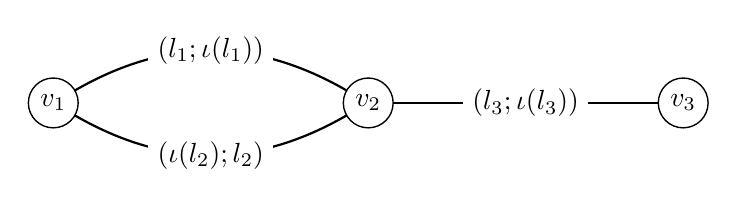
\begin{tikzpicture}
			\Vertex[x=0, y=0, L=$v_1$]{A}
			\Vertex[x=4, y=0, L=$v_2$]{B}
			\Vertex[x=8, y=0, L=$v_3$]{C}
			
			\Edge[label=$(l_3;\iota(l_3))$](B)(C)
			\tikzstyle{EdgeStyle} = [bend left]
			\Edge[label=$(l_1;\iota(l_1))$](A)(B)
			\tikzstyle{EdgeStyle} = [bend right]
			\Edge[label=$(\iota(l_2);l_2)$](A)(B)
			\end{tikzpicture}
		\end{figure}
	\end{center}
	\begin{exm}
		Consider the graph $\Gamma$ in Figure \ref{fig: example flow}, associated to a given stable curve $C$. In the picture, we denote the edge going from $v_i$ to $v_j$ as $(l_k, \iota(l_k))$ if the half-edge $l_k$ is associated to $v_i$, while we denote it with $(\iota(l_k),l_k)$ if the converse is true.
		In particular in this example we have that the edge $(l_1,\iota(l_1))$ goes from $v_1$ to $v_2,$ while the edge $(l_2,\iota(l_2))$ goes from $v_2$ to $v_1$.
		
		We have that $H_1(\Gamma,\C) \cong \C^{b_1(\Gamma)} = \C,$ while $m=3.$ For each vertex, the residue theorem translates in: \begin{enumerate}[label=(\arabic*)]
			\item $\res_{l_1}(\varphi) + \res_{\iota(l_2)}(\varphi) =0;$
			\item $\res_{\iota(l_1)}(\varphi) + \res_{l_2}(\varphi) + \res_{l_3}(\varphi)=0;$
			\item $ \res_{\iota(l_3)}(\varphi)=0.$
		\end{enumerate} Computation now follows immediately:
		$$\begin{aligned}
		\partial(\res(\varphi)) &= \partial\left(\res_{l_1}(\varphi) \ [(l_1,\iota(l_1))] + \res_{l_2}(\varphi) \ [(l_2,\iota(l_2))] + \res_{l_3}(\varphi) \ [(l_3,\iota(l_3))]\right) =\\&= \res_{l_1}(\varphi) \ [v_2] - \res_{l_1}(\varphi) \ [v_1] + \res_{l_2}(\varphi) \ [v_1] - \res_{l_2}(\varphi) \ [v_2] +\\&+ \res_{l_3}(\varphi) \ [v_3] - \res_{l_3}(\varphi) \ [v_2] = \left(\res_{l_2}(\varphi) - \res_{l_1}(\varphi)\right) [v_1] +\\&+ (\res_{l_1}(\varphi) - \res_{l_2}(\varphi) - \res_{l_3}(\varphi)) [v_2] + (\res_{l_3}(\varphi)) [v_3] =\\&= -(\res_{\iota(l_2)}(\varphi) + \res_{l_1}(\varphi)) [v_1] - (\res_{\iota(l_1)}(\varphi) + \res_{l_2}(\varphi) +\\&+ \res_{l_3}(\varphi)) [v_2] - (\res_{\iota(l_3)}(\varphi)) [v_3] = 0
		\end{aligned}$$
		
	\end{exm}
	Hence we obtained that $\Ima(\res) \subset H_1(\Gamma,\C).$\\
	Moreover, since each connected component $N_v$ of the normalization is smooth, we have that their dualizing sheaf coincides with the sheaf of holomorphic differentials, namely $\omega_{N_v} = \Omega^1_{N_v}.$ 
	If we take a holomorphic differential $\varphi \in \bigoplus_{v \in V} H^0(N_v, \Omega^1_{N_v})$, we clearly have that $\varphi \in \ker(\res)$, because $\res_{s_i}(\varphi) = \res_{s_i'}(\varphi) = 0$ for every $i$. On the other hand, if we take a meromorphic differential in the kernel, i.e. $\varphi \in H^0(C, \omega_C)$ such that $\res_{s_i}(\varphi)=0$ for every $i$, we have that, since $$\res_{s_i}(\varphi) + \res_{s_i'}(\varphi)=0,$$ also $\res_{s_i'}(\varphi)=0$ for every $i$. Since $\varphi$ has poles at most of order 1 this implies that we can see $\varphi$ as a holomorphic differential of the normalization, so we have that $\varphi \in \bigoplus_{v \in V} H^0(N_v, \Omega^1_{N_v}).$ Thus, we get that $$\ker(\res) = \bigoplus_{v \in V} H^0(N_v, \omega_{N_v}) = \bigoplus_{v \in V} H^0(N_v, \Omega^1_{N_v}).$$ 
	\begin{lemma}\label{lem: res surjective}
		The residue morphism is surjective onto $H_1(\Gamma,\C).$
	\end{lemma}
	\begin{proof}
		From Proposition \ref{relation C with G and N} and in particular from equation \eqref{eq: H1 exact sequence}, we have that the following is a short exact sequence $$0 \rightarrow H^1(\Gamma, \C) \rightarrow H^1(C,\os_C) \rightarrow \bigoplus_{v \in V} H^1(N_v, \os_{N_v}) \rightarrow 0.$$ Dualizing it we obtain $$0 \rightarrow \bigoplus_{v \in V}H^1(N_v, \os_{N_v})^\vee \rightarrow H^1(C, \os_C)^\vee \rightarrow H_1(\Gamma, \C) \rightarrow 0.$$ If we now use the generalization of Serre duality we mentioned in \eqref{eq: Serre duality}, we have that $$H^1(C, \os_C)^\vee \simeq H^0(C, \omega_C), \quad H^1(N_v, \os_{N_v})^\vee \simeq H^0(N_v, \omega_{N_v})$$ and the map on the right is actually the residue morphism. Hence we obtain the surjectivity that we wanted.
	\end{proof}
	Therefore, we have the following exact sequence \begin{equation}\label{eq: res exact sequence} 0 \rightarrow \bigoplus_{v \in V} H^0(N_v,\omega_{N_v}) \rightarrow H^0(C,\omega_C) \stackrel{\res}{\longrightarrow} H_1(\Gamma,\C) \rightarrow 0.\end{equation} 
	\begin{oss}
		Notice that, thanks to the proof of Lemma \ref{lem: res surjective}, we could have deduced at once the exact sequence in \eqref{eq: res exact sequence}. However, we decided to talk about flows, because we thought it made the situation clearer and more immediate.
	\end{oss}
	Dualizing the sequence \eqref{eq: res exact sequence}, it stays exact $$0 \rightarrow H^1(\Gamma, \C) \rightarrow H^0(C, \omega_C)^\vee \rightarrow \bigoplus_{v \in V} H^0(N_v,\omega_{N_v})^\vee \rightarrow 0.$$ By point (i) of Proposition \ref{relation C with G and N but in Z}, we have a short exact sequence $$0 \rightarrow H^1(\Gamma,\Z) \rightarrow H^1(C,\Z) \rightarrow \bigoplus_{v \in V}H^1(N_v,\Z) \rightarrow 0.$$ From the properties of the dualizing sheaf, we have that $H^0(C, \omega_C)^\vee \cong H^1(C,\os_C).$ Using this fact, we would like to give a morphism from the latter exact sequence to the former. We will give maps $H^1(\Gamma, \Z) \hookrightarrow H^1(\Gamma,\C)$ and $H^1(X,\Z) \hookrightarrow H^1(X,\os_X),$ for $X$ a connected compact curve. Consider the exponential exact sequence of $X$: $$0 \rightarrow \Z \rightarrow \os_X \stackrel{\exp}{\longrightarrow} \os_X^* \rightarrow 0,$$ where $\os_X$ is the structural sheaf of $X$ and look at the induced long exact sequence in cohomology, noticing the following properties: \begin{itemize}
		\item $H^0(X,\Z) = \Z$ being $X$ connected;
		\item $H^0(X,\os_X) = \C, H^0(X,\os_X^*) = \C^*$, being $X$ compact and connected;
		\item $H^1(X,\os_X^*) = \pic(X)$ by definition;
		\item $H^2(X,\os_X)=0$ by Grothendieck vanishing.
	\end{itemize} Hence we obtain 
	\begin{center}
		\begin{tikzcd}
			0 \arrow[r] &\Z \arrow[r] &\C  \arrow[r, "e_0"] &  \C^* \arrow[dll, out=-20, in=160, "\delta_0"] &  &\\
			& H^1(X,\Z)  \arrow[r, "j_1"] & H^1(X,\os_X) \arrow[r, "e_1"] &  \text{Pic}(X) \arrow[r, "\delta_1"] & H^2(X,\Z) \arrow[r]& 0
		\end{tikzcd}
	\end{center}
	We notice that the exponential map $e_0 \colon \C \rightarrow \C^*$ is surjective, hence we have $\C^* = \Ima(e_0) = \ker(\delta_0) \Rightarrow 0=\Ima(\delta_0) = \ker(j_1)$ which tells us that $j_1 \colon H^1(X,\Z) \hookrightarrow H^1(X,\os_X)$ is an inclusion as we wanted to show. Moreover, we have the short exact sequence $$ 0 \rightarrow \pico(N) := H^1(X,\os_X)/H^1(X,\Z) \hookrightarrow \pic(X) \twoheadrightarrow H^2(X,\Z) \rightarrow 0,$$ where we call $NS(X) := H^2(X,\Z)$ the \emph{Néron-Severi group} of $X$. \\
	
	On the other hand, we consider again the first exact part of the cohomology sequence, namely $$0 \rightarrow \Z \rightarrow \C \rightarrow \C^* \rightarrow 0.$$ Since $H^1(\Gamma,\Z)$ is free as $\Z$-module, it is also flat, hence we get the exact sequence $$0 \rightarrow H^1(\Gamma,\Z) \rightarrow H^1(\Gamma,\C) \rightarrow H^1(\Gamma,\C^*) \rightarrow 0.$$
	Thus we obtain the following commutative diagram with exact rows and columns:
	\begin{center}
		\begin{tikzcd}
			& 0 \arrow[d] & 0 \arrow[d] & 0 \arrow[d] & \\ 0 \arrow[r] & H^1(\Gamma, \Z) \arrow[r] \arrow[d, hookrightarrow] & H^1(C, \Z) \arrow[r] \arrow[d, hookrightarrow] & \bigoplus_{v \in V} H^1(N_v,\Z) \arrow[r] \arrow[d, hookrightarrow] &0 \\ 0 \arrow[r] & H^1(\Gamma, \C) \arrow[r]\arrow[d, twoheadrightarrow] & H^0(C, \omega_C)^\vee \arrow[r] \arrow[d, twoheadrightarrow] & \bigoplus_{v \in V} H^0(N_v, \omega_{N_v})^\vee \arrow[r] \arrow[d, twoheadrightarrow] & 0 \\ 0 \arrow[r] & \frac{H^1(\Gamma, \C)}{H^1(\Gamma,\Z)} \arrow[r] \isoarrow{d} & \frac{H^0(C,\omega_C)^\vee}{H^1(C,\Z)} \arrow[r] \isoarrow{d} & \bigoplus_{v \in V} \frac{H^0(N_v, \omega_{N_v})^\vee}{H^1(N_v, \Z)} \arrow[r] \isoarrow{d} & 0 \\ 0 \arrow[r] & H^1(\Gamma, \C^*) \arrow[r] & \pico(C) \arrow[r] & \bigoplus_{v \in V} \pico(N_v) \arrow[r] & 0.
		\end{tikzcd}
	\end{center}
	This diagram gives us another relevant property of the dual graph, namely the cohomology of the dual graph is able to fill in the difference between $\pico(C)$ and $\pico(N) = \bigoplus_{v \in V} \pico(N_v).$ Moreover, this allows us also to see the $\pico(C)$ as an extension of an algebraic torus, $H^1(\Gamma,\C^*) = (\C^*)^{b_1(\Gamma)}$, via an abelian variety, $\bigoplus_{v \in V} \pico(N_v)$. We call this a \emph{semi-abelian variety}.
	\newpage
\chapter{The classification of stable curves of genus 2}\label{sec: classification of stable curves genus 2}
	In this chapter, we would like to give an explicit classification in genus 2 of all the possible stable curves up to homeomorphism. In order to do so, we will look at the corresponding dual graph.
	
	This chapter is not strictly necessary for the comprehension of next sections. We still decided to write it because it gives a good example of how studying the dual graph is enough to completely classify stable curves, at least when the genus is low.\\
	
	Let $C$ be a stable curve of genus 2 and let $\Gamma =(V,E) = \text{Graph}(C)$ be its dual graph. Let $$\nu \colon N:= \bigsqcup_{v \in V} N_v \rightarrow C$$ be the normalization of $C$ where we denoted with $N_v$ the connected components of $N$.
	 
	The fact that $C$ is a stable curve implies, by definition, that its group of automorphisms is finite. This is the same as asking that $$2g(N_v) -2 + \deg(v) >0, \quad \forall \ v \in V,$$ where $g(N_v)$ is the geometric genus of $N_v$ and $\deg(v)$ is the degree of a vertex in $\Gamma$.
	
	Indeed, suppose that for each vertex $v \in V$ the inequality holds. Then we have several cases depending on the genus of the smooth irreducible component $N_v.$ \begin{itemize}
		\item If $g(N_v)\ge 2$, then it is well known that the automorphism group is finite (this is the Hurwitz automorphism theorem, see for instance Exercise IV.2.5 in \cite{MR0463157}).
		\item If $g(N_v)=1$, then $\deg(v) \ge 1$, so $N_v$ has at least one marked point (indeed, this is a point which is mapped to a node of $C$ by $\nu$) and $N_v$ is an elliptic curve. Then Corollary IV.4.7 in \cite{MR0463157} tells us that the automorphism group of $N_v$ leaving the point fixed is finite.
		\item If $g(N_v)=0$, then $N_v= \Ps^1$ and $\deg(v)\ge 3$. So $N_v$ has at least 3 marked points. An automorphism of $\Ps^1$ is completely determined by where it sends three distinct points. Since the marked points are fixed points for any automorphism of $N_v$, then the automorphism group of $N_v$ is made of at most one element and it is hence finite.
	\end{itemize}
	\begin{oss}
		We recall that we already found in Corollary \ref{cor: b1 le g} that $$b_1(\Gamma) \le g=2.$$ In fact we have from Proposition \ref{relation C with G and N but in Z} that $$2=g = b_1(\Gamma) + \sum_{v \in V} g(N_v).$$ This relation implies that $$\sum_{v \in V} g(N_v) \le g=2.$$
	\end{oss}
	We list now all the possible graphs dividing them according to the connected component with the highest genus that appears in their normalization. From the last equation we see that the highest case that we can have is 2.
	\begin{itemize}
		\item At least one component has genus 2: \\so we have that $\sum_{v \in V} g(N_v) + b_1(\Gamma)= 2 \Rightarrow g(N_{v_0})=2.$ In this case we have for sure the trivial graph (1 vertex $v_0$ and no edges) with weight 2 in the only vertex. We show now that we cannot have any other graphs. Indeed, if we have at least two vertices, we know that all vertices different from $v_0$ must have weight 0, hence should be of degree at least 3 by stability. $b_1(\Gamma)=0 \Rightarrow |E| = |V| -1$, being the graph connected this is equivalent to be a tree. Basic graph theory tells us though that a tree with at least two vertices always has at least two \emph{leaves}, i.e. vertices of degree 1. Since at least one of these two leaves must be of weight 0, this is a contradiction; hence we have only the trivial graph in this collection.
		\item At least one component has genus 1: \\suppose first that we have two vertices of weight 1, then the graph is again a tree ($b_1(\Gamma)=0$). The following lemma holds:
		\begin{lemma}
			In a tree $T$, the number of leaves is at least equal to the degree of the vertex with max degree in the tree.
		\end{lemma}
		\begin{proof}
			Let $v_0 \in V$ be the vertex with max degree, suppose it has $\deg(v_0)=k$. Then this means that $T \setminus \{v_0\}$ consists of $k$ trees, $T_i$ for $i = 1, \dots, k$ (because they must still be connected and acyclic). Each of these trees is either the trivial graph or has at least 2 leaves. In the first case, their only adjacent vertex in $T$ is $v_0$, so they were already leaves in $T$. In the second case, one of the leaves of $T_i$ must be a vertex which is adjacent to $v_0$ in $T$, while the other is a leaf also in $T$ (indeed, we only removed edges incident to $v_0$ and we do not have cycles in $T$). Hence we have at least a leaf in each connected component of $T \setminus \{v_0\}$ which is not adjacent to $v_0$ in $T$, thus they remain leaves in $T$ and we have at least $k$ leaves in $T$. This concludes the proof.
		\end{proof}
		By the lemma, if we have a vertex of weight 0 in $\Gamma$, then we should have at least 3 leaves in $\Gamma$, hence at least one of the vertices of degree 0 is a leaf, but this is a contradiction to stability. Hence the only possibility with two vertices of weight 1 is the (only) tree with 2 vertices.
		
		Suppose now that we have only one vertex $v_0$ of weight 1 and the other vertices of $\Gamma$ have weight 0. Then $b_1(\Gamma)= 1 \Rightarrow |E| = |V|$, $\deg(v_0)\ge 1$ and the handshake lemma implies that $$\begin{aligned} 2|V| = 2|E| &= \sum_{v \in V} \deg(v)  \ge \deg(v_0) + 3(|V|-1)  \ge 1 + 3|V|-3 = 3|V| -2 \\  &\Rightarrow 3|V| -2 \le 2|V| \Rightarrow  |V| \le 2.\end{aligned}$$ If $|V|=1 =|E|$, we have no choice other than a graph with vertex $v_0$ and one loop around $v_0$.\\ If $|V|=2=|E|$, we have two vertices, $v_0$ and $v$, one edge between them ($\Gamma$ must be connected) and, since $\deg(v) \ge 3$, the other edge must be a loop around $v$. %The possibilities are shown in picture \ref{picture graph genus 1}.
		\item Maximum occurring genus is 0 (hence all components have genus 0):\\ in this case we have $$2=g = \sum_{v \in V} g_v + b_1(\Gamma) = b_1(\Gamma) = |E|-|V|+1 \Rightarrow |E| = |V|+1$$ and the following lemma holds.
		\begin{lemma}
			Let $C$ be a stable curve of genus $g$ where all irreducible components $N_v$ of the normalization of $C$ have genus $g_v:= g(N_v)=0.$ Then $$|E| := |E(\Gamma)| \le 3g-3.$$
		\end{lemma}
		\begin{proof}
			Since $C$ is stable, we have, for all $v \in V$ that $$2g_v -2 + \deg(v) >0 \Rightarrow \deg(v) \ge 3.$$ The handshake lemma tells us that $$2|E| = \sum_{v \in V} \deg(v) \ge 3|V|.$$ The formula for the genus of $C$ becomes $$g = b_1(\Gamma) + \sum_{v \in V} g_v = b_1(\Gamma) = |E| - |V| +1.$$ Multiplying it by 3, we get $$3g -3 = 3|E| - 3|V| \ge 3|E| - 2|E| = |E|.$$
		\end{proof}
		In our case this tells us that $|E| \le 3.$ By handshake lemma, this implies that $|V| \le 2.$ \\If $|V|=2$, then $|E|=3$ and in order to satisfy the stability and connectivity conditions, we should have either one edge between the two vertices and one loop around each of them or three edges between them.\\
		If $|V|=1$, then $|E|=2$ and the only possibility is having two loops around this vertex. %These cases are shown in picture \ref{picture graph genus 0}.
	\end{itemize}
	
	So in total we have 7 possible cases, which are shown in Figure \ref{pic: stable genus 2}.
	%\begin{figure}[h!] 
		
	%	\begin{tikzpicture}[scale=0.75, transform shape]
	%	\Vertex[x=0,y=0]{2}
	%	\end{tikzpicture}
	%	\begin{tikzpicture}[scale=0.75, transform shape]
	%	\Vertex[x=0,y=0, L = 1]{A}
	%	\Loop(A)
	%	\end{tikzpicture}
	%	\begin{tikzpicture}[scale=0.75, transform shape]
	%	\Vertex[x=0,y=0, L=0]{A}
	%	\Vertex[x=2, y=0,L=1]{B}
	%	\Edge(A)(B)
	%	\Loop(A)
	%	\end{tikzpicture}
	%	\begin{tikzpicture}
	%	\Vertex[x=0,y=0, L=1]{A}
	%	\Vertex[x=2, y=0, L=1]{B}
	%	\Edge(A)(B)
	%	\end{tikzpicture}
	%	\begin{tikzpicture}
	%	\Vertex[x=0,y=0,L=0]{A}
	%	\Vertex[x=2, y=0, L=0]{B}
	%	\Edge(A)(B)
	%	\tikzstyle{EdgeStyle} = [bend left]
	%	\Edge(A)(B)
	%	\tikzstyle{EdgeStyle} = [bend right]
	%	\Edge(A)(B)
	%	\end{tikzpicture}
	%	\begin{tikzpicture}
	%	\Vertex[x=0,y=0,L=0]{A}
	%	\Vertex[x=2,y=0, L=0]{B}
	%	\Edge(A)(B)
	%	\Loop(A)
	%	\Loop[dir=EA](B)
	%	\end{tikzpicture}
	%	\begin{tikzpicture}
	%	\Vertex[x=1,y=0,L=0]{A}
	%	\Loop(A)
	%	\Loop[dir=EA](A)
	%	\end{tikzpicture}
	%\end{figure}
	\begin{figure}[h!]
		\caption{The graphs associated to the 7 stable curves of genus 2}
		\label{pic: stable genus 2}
		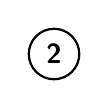
\begin{tikzpicture}[auto,node distance= 3cm, thick,main node/.style={circle,draw,font=\sffamily\bfseries},every loop/.style={}]
		\node[main node] (1) {2};
		\end{tikzpicture}
		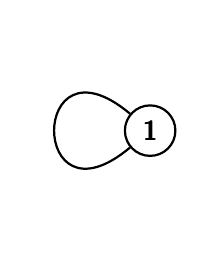
\begin{tikzpicture}[auto,node distance= 3cm, thick,main node/.style={circle,draw,font=\sffamily\bfseries},every loop/.style={}]
		\node[main node] (1) {1};
		\path[every node/.style={font=\sffamily\small}]
		(1) edge [out=220,in=140,looseness=10] node {} (1);
		\end{tikzpicture}
		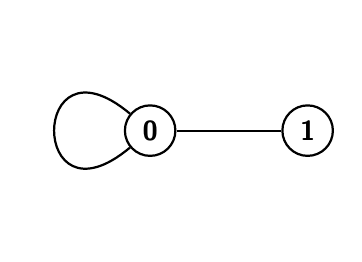
\begin{tikzpicture}[auto,node distance= 2cm, thick,main node/.style={circle,draw,font=\sffamily\bfseries},every loop/.style={}]
		\node[main node] (1) {0};
		\node[main node] (2) [right of =1] {1};
		\path[every node/.style={font=\sffamily\small}]
		(1) edge node {} (2)
		 edge [out=220,in=140,looseness=10] node {} (1);
		\end{tikzpicture}
		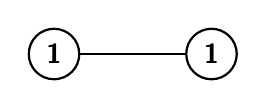
\begin{tikzpicture}[auto,node distance= 2cm, thick,main node/.style={circle,draw,font=\sffamily\bfseries},every loop/.style={}]
		\node[main node] (1) {1};
		\node[main node] (2) [right of =1] {1};
		\path[every node/.style={font=\sffamily\small}]
		(1) edge node {} (2);
		\end{tikzpicture}
		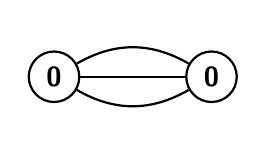
\begin{tikzpicture}[auto,node distance= 2cm, thick,main node/.style={circle,draw,font=\sffamily\bfseries},every loop/.style={}]
		\node[main node] (1) {0};
		\node[main node] (2) [right of =1] {0};
		\path[every node/.style={font=\sffamily\small}]
		(1) edge node {} (2)
		edge [bend right] node {} (2)
		edge [bend left] node {} (2);
		\end{tikzpicture}
		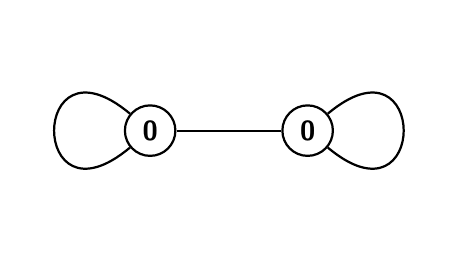
\begin{tikzpicture}[auto,node distance= 2cm, thick,main node/.style={circle,draw,font=\sffamily\bfseries},every loop/.style={}]
		\node[main node] (1) {0};
		\node[main node] (2) [right of =1] {0};
		\path[every node/.style={font=\sffamily\small}]
		(1) edge node {} (2)
		edge [out=220,in=140,looseness=10] node {} (1)
		(2) edge [out=40, in=-40, looseness=10] node {} (2);
		\end{tikzpicture}
		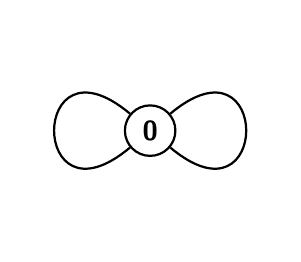
\begin{tikzpicture}[auto,node distance= 2cm, thick,main node/.style={circle,draw,font=\sffamily\bfseries},every loop/.style={}]
		\node[main node] (1) {0};
		\path[every node/.style={font=\sffamily\small}]
		(1) edge [out=220,in=140,looseness=10] node {} (1)
		edge [out=40,in=-40,looseness=10] node {} (1);
		\end{tikzpicture}
	\end{figure}
\newpage
\chapter{The monodromy pairing}\label{monodromy pairing}
In this chapter we study the monodromy action induced on the homology of a smooth fiber of a family of stable curves over a polydisk $f \colon X \rightarrow B$. We already introduced this action in chapter \ref{sec: picard-lefschetz theory}, but we now deduce from it a pairing on the homology of the dual graph $\Gamma$ associated to the central fiber $X_0$ of the family $f$. We then define the cycle pairing $M_e$, again on the homology of the dual graph $\Gamma$, and we show that these two pairings are actually identical. We follow in doing this section 3.2 of \cite{MR3588803}.\\
	
	Fix a universal family of curves with stable degeneration $f \colon X \rightarrow B$, where $B:= \Delta^r$ is a polydisk of dimension $r$. 
	
	Suppose that the central fiber $X_0$ has smooth irreducible components $X_v$, where these components are indexed via the set of vertices of the dual graph $\Gamma = \text{Graph}(X_0) =(V,E)$ associated to $X_0$. Hence, we have the normalization map $$\nu \colon \coprod_{v \in V} X_v \twoheadrightarrow X_0,$$ which identifies $X_0$ as a quotient of $\coprod_{v \in V}X_v$ obtained identifying points of different components that are glued together after $\nu$.
	In particular, we recall that these identifications correspond one-to-one to edges in the dual graph $\Gamma$. 
	
	Since the family has stable degeneration, we have a normal crossings divisor $D \subset B$ defined locally by the equation $\{\prod_{e \in E} f_e=0\}.$ Take now a point $b_0 \in B \setminus D$ whose fiber $X_{b_0}$ is smooth. We want to study the monodromy action on $H_1(X_{b_0},\Z)$. In order to achieve this, we take for each edge of $\Gamma$ a simple loop $l_e \subset B \setminus D$ based at $b_0$ which winds simply only around the irreducible component $\{f_e =0\} \subset D$ (this assumption means that in $B \setminus \{\prod_{d \in E \setminus e} f_d =0\}$ the loop $l_e$ becomes contractible). By \ref{prop: monodromy associated to picard lefschetz representation}, the monodromy for the action of $l_e$ on $H_1(X_{b_0},\Z)$ corresponds to a Dehn twist along the vanishing cycle $c_e \in H_1(X_{b_0},\Z)$ associated to the edge $e \in E$ and so is given by the Picard-Lefschetz formula $$T_e :=H_1(l_e) \colon H_1(X_{b_0},\Z) \rightarrow H_1(X_{b_0},\Z), \quad b \mapsto b + Q (b, c_e) c_e,$$ where we use $Q \colon H_1(X_{b_0},\Z) \times H_1(X_{b_0},\Z) \rightarrow \Z$ to indicate the intersection pairing.
	We recall that from section \ref{sec: cohomology dual graph} we have a surjective map $$\rho_* \colon H_1(X_{b_0},\Z) \twoheadrightarrow H_1(X_0,\Z),$$ obtained via functoriality composing the inclusion $X_{b_0} \hookrightarrow X$ with the retraction $X \rightarrow X_0$. This map is surjective because of Proposition \ref{prop: relation X0 and Xb0}. To see this intuitively, one can divide a cycle in $H_1(X_0,\Z)$ into segments which connect double points of the curve. Each of these segments lives inside one of the irreducible components $X_v$. Hence we can "lift" them to segments in $H_1(X_{b_0},\Z)$ and glue them along the vanishing cycles, so that their image is the cycle we started with.
	
	Call $A$ the subspace of $H_1(X_{b_0},\Z)$ generated by the vanishing cycles $c_e$. We know from Proposition \ref{prop: relation X0 and Xb0} that we have a short exact sequence given by $$0 \rightarrow A \rightarrow H_1(X_{b_0},\Z) \stackrel{\rho_*}{\longrightarrow} H_1(X_0,\Z) \rightarrow 0.$$ Define $$A' := \rho_*^{-1}\left( \bigoplus_{v \in V} H_1(X_v,\Z)\right) \subset H_1(X_{b_0},\Z).$$ 
	\begin{lemma}\label{lem: A' is A plus the normalization homology}
		We have that $$A' \simeq A \oplus \bigoplus_{v \in V} H_1(X_v,\Z).$$
	\end{lemma}
	\begin{proof}
		Consider the following short exact sequence: $$0 \rightarrow \ker \rho_* \rightarrow \rho_*^{-1}\left( \bigoplus_{v \in V} H_1(X_v,\Z)\right) \stackrel{\rho_*}{\longrightarrow}  \bigoplus_{v \in V} H_1(X_v,\Z) \rightarrow 0.$$ We know that $\ker \rho_* = A$; since $\bigoplus_{v \in V} H_1(X_v,\Z)$ is a free $\Z$-module, the sequence is split and so $$A' := \rho_*^{-1}\left( \bigoplus_{v \in V} H_1(X_v,\Z)\right) \simeq A \oplus \bigoplus_{v \in V} H_1(X_v,\Z).$$ 
	\end{proof}
	\begin{oss}
		From Lemma \ref{lem: A' is A plus the normalization homology} we get that $A \subset A'.$
	\end{oss}
	We have the following chain of isomorphisms: $$H_1(X_{b_0},\Z)/A' \cong H_1(X_0,\Z)/ \bigoplus_{v \in V} H_1(X_v,\Z) \cong H_1(\Gamma,\Z).$$ The second isomorphism descends from the discussion before formula \ref{g(C)} recalling that $b_1(\Gamma)= \rk H_1(\Gamma,\Z)$; while the first one follows from the previous exact sequence, because $$H_1(X_{b_0},\Z)/\left(\rho_*^{-1}( \bigoplus_{v \in V} H_1(X_v,\Z))\right) \cong H_1(X_0,\Z) / \bigoplus_{v \in V} H_1(X_v,\Z)$$ and the isomorphism is given applying $\rho_*$.
	\begin{lemma}
		The subspace $A \subset H_1(X_{b_0},\Z)$ is isotropic with respect to the intersection pairing, i.e. for every $a,b \in A,$ we have $Q(a,b)=0$, and $A$ has rank $b_1(\Gamma).$
	\end{lemma}
	\begin{proof}
		Up to moving the point $b_0 \in B \setminus \cup_{e \in E} D_e$, we can suppose the vanishing cycles in $X_{b_0}$ to be disjoint, hence $Q(c_e,c_{e'})=0$ for every $e\neq e' \in E.$ Moreover, since the intersection pairing is a symplectic form, we get that $Q( c_e,c_e) =0$ for every $e \in E.$ Hence $A$ is isotropic. Now we compute its rank. From Proposition \ref{prop: relation X0 and Xb0} (setting $R=\Z$), we have that $A \simeq H^1(\Gamma,\Z)$. Thus, by Proposition \ref{prop: rank is betti}, we obtain that$$\rk A = \rk H^1(\Gamma,\Z) = b_1(\Gamma).$$
	\end{proof}
	Actually we have something more, indeed $A \simeq (A')^\bot$, where $(A')^\bot$ is the orthogonal complement of $A$ with respect to the intersection pairing $Q$.
	\begin{lemma}
		$$A \simeq (A')^\bot.$$
	\end{lemma}
	\begin{proof}
		First, we have that $A \subset (A')^\bot$. Indeed, $Q(A,A')=0,$ because, for $a \in A, b \in \rho_*^{-1}\left(\bigoplus_{v \in V} H_1(X_v,\Z)\right)$, we have that we can always stretch $b$ such that it does not intersect any vanishing cycle, hence $Q(a,b)=0.$
		Tensoring with $\Q$, we get that $$\dim (A')^\bot \otimes \Q = \dim H_1(X_{b_0},\Q) - \dim A' \otimes \Q.$$ The same formula holds for the ranks, as all modules are free over a PID: $$\rk (A')^\bot = \rk H_1(X_{b_0},\Z) - \rk A'.$$ From Lemma \ref{lem: A' is A plus the normalization homology} we have that $$\rk A' = \rk A + \rk \bigoplus_{v \in V} H_1(X_v,\Z) = b_1(\Gamma) + 2 \sum_{v \in V} g_v.$$ Hence we get that $$\rk (A')^\bot = 2g(X_{b_0}) - b_1(\Gamma) - 2 \sum_{v \in V} g_v.$$ By equation \eqref{eq: relation between genera of Xb0, b1Gamma and sum Xv}, we get that $g(X_{b_0}) = b_1(\Gamma) + \sum_{v \in V} g_v.$ Therefore, $$\rk(A')^\bot = 2b_1(\Gamma) + 2\sum_{v \in V} g_v - b_1(\Gamma) -2\sum_{v \in V} g_v = b_1(\Gamma) = \rk A.$$
		Tensoring with $\Q$, we have that $$\dim \left(\frac{(A')^\perp \otimes \Q}{A \otimes \Q}\right) = 0 \ \Rightarrow \ \rk \left(\frac{(A')^\perp}{A}\right)
		 =0.$$ Since $(A')^\perp \subset H_1(X_{b_0},\Z)$ and $H_1(X_{b_0},\Z) /A \simeq H_1(X_0,\Z)$ is a free module, then we have that $(A')^\perp /A \subset H_1(X_{b_0},\Z)/A$ is torsion-free and of rank zero.
		
		 Thus, $A \simeq (A')^\bot.$
	\end{proof}
	We have the following lemma about perfect pairings: 
	\begin{lemma}
		Let $V,W$ be two free $\Z$-modules of finite rank. Suppose that it is given a perfect pairing $$P \colon V \times W \rightarrow \Z.$$ Let $B \subset V$ be a submodule such that $V/B$ is torsion-free and let $B^\perp \subset W$ be its orthogonal complement with respect to $P$. Then $P$ induces a perfect pairing $$\left(V/B\right) \times B^\perp \rightarrow \Z.$$
	\end{lemma}
	\begin{proof}
		Restricting $P$ to $V \times B^\perp$, we get a pairing $P \colon V \times B^\perp \rightarrow \Z.$ We are interested though in the map $$P \colon V \rightarrow (B^\perp)^\vee := \Hom(B^\perp,\Z).$$ Clearly its kernel is given by $(B^\perp)^\perp.$ So there is an induced injective map $$P \colon \frac{V}{(B^\perp)^\perp} \rightarrow (B^\perp)^\vee.$$ We show that it is an isomorphism. 
		
		Indeed, it is surjective: take $f \in \Hom(B^\perp,\Z);$ lift $f$ to a map $\tilde{f} \in \Hom(W,\Z) = W^\vee.$ Since $P$ is a perfect pairing on $V\times W$, there exists $v \in V$ such that $\tilde{f} = P(v,-).$ Restricting ourselves to $V \times B^\perp$ we get that $P(v,-) = f.$
		
		To prove that $B = (B^\perp)^\perp$ we need to use the fact that $V/B$ is torsion-free. Indeed, we clearly have that $B \subseteq (B^\perp)^\perp.$ Tensoring with $\Q$ over $\Z$, we get two vector spaces of the same dimension, hence $\rk B = \rk (B^\perp)^\perp$. Passing again to the $\Q$-vector spaces we also have that $\rk\left((B^\perp)^\perp/B\right) = 0.$ As $(B^\perp)^\perp/B \subset V/B$, we get that $(B^\perp)^\perp/B$ is torsion-free and of rank zero. Hence $B = (B^\perp)^\perp.$ The result then follows.
	\end{proof}
	We can apply the previous lemma to $V=W= H_1(X_{b_0},\Z), P = Q, B=A'.$\footnote{Notice that $V/A' = H_1(X_{b_0},\Z)/ A' \simeq H_1(\Gamma,\Z)$ is free, hence also torsion-free.}
	Thus, since $A \subset H_1(X_{b_0},\Z)$ is the orthogonal to $A'$ with respect to the intersection pairing (which is perfect by Remark \ref{rmk: intersection pairing is perfect}), we obtain that the intersection pairing induces a perfect pairing $$Q \colon A \times \frac{H_1(X_{b_0},\Z)}{A'} \rightarrow \Z.$$
	Define now a map $$N_e \colon H_1(X_{b_0},\Z) \rightarrow H_1(X_{b_0},\Z), \quad N_e = T_e-\id,$$ where we recall that $T_e = H_1(l_e)$ is a Dehn twist along the vanishing cycle $c_e$ corresponding to $e \in E$. For every $\beta \in H_1(X_{b_0},\Z)$, we have that $$N_e(\beta)= \beta + Q(\beta, c_e) c_e - \beta=  Q(\beta, c_e) c_e.$$ Thus $\Ima N_e \subset A$, while $\ker N_e \supset A' \supset A.$
	\begin{oss}
		Since we showed that $N_e \colon H_1(X_{b_0},\Z) \rightarrow A$ and $A \subset \ker N_e$, then we obtain that $N_e^2=0.$ Using Taylor expansion, this implies that $$\log(T_e) = \log (N_e +\id) = N_e - \frac{N_e^2}{2} + o(N_e^2) = N_e.$$
		We are justified then to call $N_e$ the \emph{logarithm operator} associated to the monodromy operator $T_e.$ We will see again this language when we will talk about the asymptotic height pairing in chapter \ref{sec: ahp}.
		%Attento: sii sicuro di parlarne dopo e non prima.
	\end{oss}
	Using the induced perfect pairing and the fact that $N_e$ factors through the quotient by $A'$, we get that $$H_1(\Gamma,\Z) \cong H_1(X_{b_0},\Z)/A' \stackrel{N_e}{\longrightarrow} A \cong (H_1(X_{b_0},\Z)/A')^\vee \cong H_1(\Gamma,\Z)^\vee.$$
	\begin{defn}
		We just showed that there is a bilinear form associated to $N_e$, which we will call \emph{the monodromy pairing} and denote again with $N_e$ and that is given by $$N_e \colon H_1(\Gamma, \Z) \times H_1(\Gamma,\Z) \rightarrow \Z, \quad (a,b) \mapsto Q(a, N_e(b)) = Q(a, Q(b,c_e)c_e).$$
	\end{defn} 
	Before stating and proving the proposition which provides a relation between the monodromy and the combinatorics of the graph $\Gamma$, we should talk about another bilinear form, namely the \emph{cycle pairing}.
	\begin{defn}\label{def: bilnear form Me}
		For $e \in E,$ define the \emph{cycle pairing} $$M_e \colon C_1(\Gamma,\Z) \times C_1(\Gamma,\Z) \rightarrow \Z, \quad \left(\sum_{f \in E} a_f \ [f], \sum_{f \in E} b_f \ [f]\right) \mapsto a_e b_e.$$
		This induces another pairing on $H_1(\Gamma,\Z) \subset C_1(\Gamma,\Z)$ which we will call again, by abuse of notation, $M_e \colon H_1(\Gamma,\Z) \times H_1(\Gamma,\Z) \rightarrow  \Z.$
	\end{defn}
	\begin{prop}\label{prop: Ne = Me}
		The monodromy pairing $N_e$ on $H_1(\Gamma,\Z)$ coincides with the cycle pairing $M_e$.
	\end{prop}
	\begin{proof}
		Take $a,b \in H_1(X_{b_0},\Z)$. In the quotient $\psi \colon H_1(X_{b_0},\Z)/A' \stackrel{\sim}{\longrightarrow} H_1(\Gamma,\Z)$, we can identify $a$ with a cycle $\psi(a) = \sum_{e \in E} m_e e,$ where $m_e = Q(a, c_e).$ This is because the map $\rho_*$ leaves $a$ almost invariate, except it contracts the vanishing cycles $c_e$ to the node $p$; in $\Gamma$, the irreducible components are contracted to vertices, so $a$ becomes just a linear combination of edges; because what matters in $\Gamma$ is only how many times and in which way $a$ crosses each vanishing cycle $c_e.$ In the same way, we get that $\psi(b) = \sum_{e \in E} n_e e$, where $n_e= Q(b,c_e)$. Thus, we obtain on $H_1(X_{b_0},\Z)$ (the same is true if we pass to the quotient, i.e. if we work on $H_1(\Gamma,\Z)$) that $$N_e(a,b) = Q(a, Q(b, c_e) c_e ) = Q(b,c_e) Q(a,c_e)= m_e n_e.$$ On the other hand, we have $$M_e(\psi(a),\psi(b)) = M_e \left(\sum_{f \in E} m_f f, \sum_{f \in E} n_f f\right) = m_e n_e .$$
	\end{proof}
	We can fix a symplectic basis $\{a_1, \dots, a_g, b_1, \dots, b_g\}$ such that  $$H_1(X_{b_0},\Z) = \Span_\Z(a_1,\dots, a_g, b_1, \dots, b_g), \quad A = \Span_\Z(a_1, \dots, a_{b_1(\Gamma)}).$$ Hence we can write, for any $e \in E$, $$c_e = \sum_{i=1}^{b_1(\Gamma)}c_{e,i}a_i.$$ Define now the subspace $B := \Span_\Z(b_1, \dots, b_{b_1(\Gamma)}) \subset H_1(X_{b_0},\Z)$, where $b_j \in H_1(X_{b_0},\Z)$ are such that $Q(a_i, b_j ) = \delta_{i,j}.$ Because of dimension reasons and previous discussions, we have that $$B \simeq A^\vee \simeq H_1(\Gamma,\Z).$$ Thus we can see the logarithm operators as maps $$N_e \colon B \rightarrow A.$$ \begin{prop}
		In terms of the basis $\{b_1, \dots, b_{b_1(\Gamma)}\}$ for $B \simeq H_1(\Gamma,\Z)$, we have that $$M_e = \left(c_{e,i} c_{e,j}\right)_{i,j}.$$
	\end{prop}
	\begin{proof}
		Taken $b_i \in \{b_1, \dots, b_{b_1(\Gamma)}\}$, one has that $$N_e(b_i) = Q(c_e, b_i) c_e = \sum_{j=1}^{b_1(\Gamma)} c_{e,j} Q\left(\sum_{k=1}^{b_1(\Gamma)} c_{e,k} a_k ,b_i \right) a_j = \sum_{j=1}^{b_1(\Gamma)} c_{e,j} c_{e,i} a_j.$$ Hence the matrix associated to this bilinear form is $\left(c_{e,i} c_{e,j}\right)$. Moreover, we showed that the bilinear form associated to $N_e$ coincides with the bilinear form $M_e$. This concludes the proof.
	\end{proof}
	\newpage
	
\chapter{The asymptotic height pairing}\label{sec: ahp}
	In this chapter, we want to introduce the asymptotic height pairing in a general context, as is done in section 6 of \cite{MR3983292}. Doing this will take some time, as we first need to define the necessary machinery. 
	
	Fix a field $\F$. Let $E$ be a $\F$-vector space of dimension $r$ with basis $\{e_1, \dots, e_r\}.$ Let $L$ be a $\F$-vector space with endomorphisms $T_i \colon L \rightarrow L$, for $i=1, \dots, r$ and logarithm operators $N_i = T_i - \id \colon L \rightarrow L$ for $i=1, \dots, r.$ 
	
	Consider the Koszul complex $K^\bullet(L) := L \otimes \bigwedge^\bullet E$, with differential $$d \colon L \otimes \bigwedge^m E \rightarrow L \otimes \bigwedge^{m+1} E, \quad d(l \otimes \omega) := \sum_{i=1}^r N_i l \otimes (e_i \wedge \omega).$$ In particular, we have that $K^0(L) = L,$ hence for $m=0$, the differential becomes $$d \colon L \rightarrow L \otimes E, \quad l \mapsto \sum_{i=1}^r N_il \otimes e_i.$$ For a multi-index $J = (j_1, \dots, j_p),$ with $1 \le j_1 < \dots < j_p \le r$, we denote $N_J = N_{j_1} \dots N_{j_p}$ and $e_J = e_{j_1} \wedge \dots \wedge e_{j_p}.$
	\begin{defn}
		We define the \emph{partial Koszul complex} as the subcomplex $B^\bullet(L) \subset K^\bullet(L)$ generated by the elements of the form $\sum_J N_J(l) \otimes e_J$ for $l \in L.$ 
	\end{defn}
	Let $\Delta^r$ denote the polydisk with coordinates $(s_1, \dots, s_r)$, $D$ be the divisor defined by $\{s_1 \cdot \dots \cdot s_r =0\} \subset \Delta^r$ and $(\Delta^*)^r := \Delta^r \setminus D.$ Let $\ls$ be the local system of $\F$-vector spaces on $(\Delta^*)^r$ whose general fiber is $L$. By \eqref{eq: equivalence local systems and representations}, we can associate to $\ls$ monodromy operators $T_i \colon L \rightarrow L$ and logarithm operators $N_i = \log T_i$ for $i=1, \dots, r.$
	The partial Koszul complex $B^\bullet(L)$ computes the intersection cohomology groups $\IH^\bullet(\mathcal{L}) = \IH^\bullet(\Delta^{r}, \mathcal{L})$, while the complex $K^\bullet(L)$ computes the sheaf cohomology groups $H^\bullet(\mathcal{L}) = H^\bullet((\Delta^*)^r, \mathcal{L}).$
	\begin{oss}
		The complexes $K^\bullet(L)$ and $B^\bullet(L)$ depend only on $\{L, N_1, \dots, N_r\}.$
	\end{oss}
	Let $t \in \F^r$. We set $N(t) := \sum_{i=1}^r t_iN_i \colon L \rightarrow L$. %and we write $\mathcal{L}_t$ for the local system on $\Delta^{*}$ with monodromy operators
	For $\alpha = \sum_{i=1}^r \alpha_i \otimes e_i \in K^1(L)$, with $\alpha_i \in L$, and $t \in \F^r$ we write $\alpha(t) := \sum_{i=1}^r t_i \alpha_i \in L.$ \\
	\textbf{Assumption}\label{assumption mhs} From now on, we suppose that $\F$ is either $\Q$ or $\R.$ Moreover, we assume that $L$ comes with an additional mixed Hodge structure such that $N_i \colon L \rightarrow L$ are a morphism of mixed Hodge structure for every $i =1, \dots, r.$
	
	The following is Proposition 120 in \cite{MR3983292}:
	\begin{prop}\label{N(t)l(t)}
		Let $\alpha= \sum_{i=1}^r \alpha_i \otimes e_i \in Z^1(B^\bullet(L)) = \{\alpha \in B^1(L) \mid d\alpha =0\}$ be a representative of an intersection cohomology class. Then for every $t \in \F^r_{\ge 0}$ there exists an element $l(t) \in L$ such that $$\alpha(t) = N(t)l(t).$$
	\end{prop}
	\begin{oss}\label{rmk: mhs}
		Suppose that $L := H_1(Y_b, \F)$, for $f \colon Y \rightarrow B$ a family of curves with stable degeneration over a polydisk $B:= \Delta^r$ with a normal crossings divisor $D =\{s_1 \cdots s_r=0\} \subset B$ (where $s_i$ are the local coordinates on the polydisk). This is the case we will focus on in this master thesis. In this setting, $L$ actually comes with a mixed Hodge structure such that the logarithm operators $N_i$ are a morphism of mixed Hodge structures, as it is mentioned at the beginning of section 4 of \cite{MR2059020}. Hence, the hypothesis of Proposition \ref{N(t)l(t)} is satisfied in this case.
	\end{oss}
	\begin{defn}
		For $X \in E^*,$ where $E^*$ denotes the dual of $E$ with dual basis $\{e_1^*, \dots, e_r^*\},$ we have the interior product $$\iota_X \colon \bigwedge^p E \rightarrow \bigwedge^{p-1} E.$$ The same $X$ also gives a morphism $$\delta_X \colon K^p(L) \rightarrow K^{p-1}(L), \quad \delta_X(l \otimes \omega) \mapsto l \otimes \iota_X(\omega).$$
		For $t=(t_1,\dots, t_r) \in \F^r$, we write $X(t) := \sum_{i=1}^r t_i e_i^*$ and we define $\delta_t := \delta_{X(t)}$. In particular, for $p=1$, we have $$\delta_t \colon L \otimes E \rightarrow E, \quad l\otimes e_i \mapsto t_i l.$$
		We set $\Delta_t := d \delta_t + \delta_t d \in \text{End}(K^\bullet(L)).$
	\end{defn}
	\begin{oss}
		For $\alpha = \sum_{i=1}^r \alpha_i \otimes e_i \in L \otimes E$, we have $$\delta_t \alpha = \sum_{i=1}^r t_i \alpha_i = \alpha(t).$$
	\end{oss}
	\begin{lemma}
		Let $t \in \F^r$ and define an operator $$N(t) \colon K^p(L) \rightarrow K^p(L), \quad h \otimes \omega \mapsto (N(t)h)\otimes \omega.$$ Then $\Delta_t = N(t).$
	\end{lemma}
	\begin{proof}
		We recall that the interior product satisfies the following graded Leibniz rule, where $\beta$ is a $p$-form and $\gamma$ is a $q$-form : $$ \iota_X(\beta\wedge\gamma) = (\iota_X\beta)\wedge\gamma+(-1)^p\beta\wedge(\iota_X\gamma).$$ Moreover, we have that $$\iota_{X(t)}(e_i) = e_i\left(\sum_{j=1}^r t_j e_j^*\right) = \sum_{j=1}^r t_j e_j^*(e_i) = t_i.$$
		Hence, we get $$\begin{aligned}
		\Delta_t(l \otimes \omega) &= d \delta_t (l \otimes \omega) + \delta_t d (l \otimes \omega) = d (l \otimes \iota_{X(t)}(\omega)) + \delta_t\left(\sum_{i=1}^r N_il \otimes (e_i \wedge \omega)\right) = \\ &= \sum_{i=1}^r N_i l \otimes (e_i \wedge \iota_{X(t)}(\omega)) + \sum_{i=1}^r N_il \otimes \iota_{X(t)}(e_i \wedge \omega) =\\&= \sum_{i=1}^r N_i l \otimes \left(e_i \wedge \iota_{X(t)} + \iota_{X(t)}(e_i \wedge \omega)\right) =\\&= \sum_{i=1}^r N_il \otimes \left(e_i \wedge \iota_{X(t)}(\omega) + \iota_{X(t)}(e_i) \wedge \omega - e_i \wedge \iota_{X(t)}(\omega)\right) =\\&= \sum_{i=1}^r N_i l \otimes (\iota_{X(t)}(e_i) \wedge \omega) =\\&= \sum_{i=1}^r N_i l \otimes t_i \omega = \sum_{i=1}^r N_i t_i l \otimes \omega = (N(t) l )\otimes \omega = N(t)(l \otimes \omega).
		\end{aligned}$$
	\end{proof}
	We want to define a pairing on the partial Koszul complex. \\
	\textbf{Notation} Suppose $I=(i_1, \dots, i_k)$ is a multi-index with $1 \le i_1 < \dots <i_k \le r,$ then for $t= (t_1, \dots, t_r) \in \F^r$ we denote with $t_I= t_{i_1} t_{i_2} \cdot \dots \cdot t_{i_k}.$ We denote with $L^*$ the dual vector space of $L$.
	\begin{defn}
		We have the following pairing $q(t) \colon B^p(L) \otimes B^p(L^*) \rightarrow \F$ given by $$q(t)\left(N_I l\otimes e_I, N_J^* \lambda \otimes e_J\right) = \begin{cases} t_I(l, N_J^*\lambda)= t_J(N_Il, \lambda) \quad \text{if } I=J;\\ 0 \quad \text{if } I\neq J.\end{cases}$$
	\end{defn}
	The pairing $q(t)$ is well defined, indeed if $I=J$, we have that $$t_I(l, N_J^*\lambda) = t_IN_J^*\lambda(l) = t_J \lambda(N_I l) = t_J(N_I l , \lambda).$$
	\begin{exm}
		For $p=1$, we have that the pairing becomes $q(t) \colon B^1(L) \otimes B^1(L^*) \rightarrow \F$, given by $$q_t(N_i l \otimes e_i, N_j^* \lambda \otimes e_j) = \begin{cases}
		t_j(l, N_j^*\lambda) = t_i(N_il, \lambda) \quad \text{if } i=j;\\ 0 \quad \text{otherwise}.
		\end{cases}$$
	\end{exm}
	\begin{prop}\label{pseudosymmetry}
		For $\alpha \in B(L), \beta \in B(L^*), t \in \F^r$, then \begin{enumerate}[label=(\arabic*)]
			\item $q(t)(d\alpha, \beta) = q(t)(\alpha, \delta_t \beta);$
			\item $q(t)(\delta_t\alpha, \beta) = q(t)(\alpha, d\beta)$.
		\end{enumerate}
	\end{prop}
	\begin{proof}
		First we notice that (2) is symmetric to (1), given the double description that we gave of $q(t)$; hence we will prove just (1). Let $\alpha = N_J l \otimes e_J, \beta = N_K^* \lambda \otimes e_K,$ for $J,K$ multi-indices on $\{1, \dots, r\}.$ We have that $$d\alpha = \sum_{i=1}^r N_i N_J l \otimes (e_i \wedge e_J).$$ From the definition, $q(t)(d\alpha, \beta) \neq 0$ if and only if $e_i \wedge e_J = \epsi e_K$, where $\epsi =\pm 1.$ We focus on this case, because otherwise the result is immediate. Since $e_i \wedge e_J = \epsi e_K,$ we get that $N_i N_J = N_K$ and $t_i t_J = t_K.$ Thus $$q(t)(d\alpha, \beta) = q(t)(N_i N_J l \otimes (e_i\wedge e_J), N_K^*\lambda \otimes e_K) = \epsi q(t)(N_Kl \otimes e_K, N_K^* \lambda \otimes e_K) = \epsi t_K(l, N_K^* \lambda).$$ On the other hand, $$\begin{aligned} q(t)(\alpha, \delta_t \beta) &= q(t)(N_J l \otimes e_J, \epsi N_K^* \lambda \otimes \iota_{X(t)}(e_i \wedge e_J)) = q(t)(N_J l \otimes e_J, \epsi N_K^* \lambda \otimes t_i e_J) =\\&= \epsi t_i q(t)(N_J l \otimes e_J, N_K^*\lambda \otimes e_J) = \epsi t_i t_J (l, N_K^* \lambda) = \epsi t_K (l, N_K^* \lambda). \end{aligned}$$
	\end{proof}
	\begin{prop}\label{alpha'}
		Let $\alpha \in Z^1(B^\bullet(L))$ represent a cohomology class, let $t \in \F^r_{\ge 0}$. By Proposition \ref{N(t)l(t)} there exists $l(t) \in L$ such that $\alpha(t) = N(t)l(t).$ Set $\alpha' := \alpha - dl(t) \in Z^1(B^\bullet(L)).$ Then, $\alpha'$ has the same image as $\alpha$ in cohomology and $\alpha' \in \ker \delta_t.$
	\end{prop}
	\begin{proof}
		First, we check that $\alpha' \in Z^1(B^\bullet(L)):$ $$d\alpha' = d\alpha - d^2l(t) =0.$$
		Clearly, since $dl(t) \in \Ima(d)$, we know that $\alpha,\alpha'$ have the same image in cohomology. So we are left to show that $\delta_t \alpha' = 0:$ $$\delta_t \alpha' = \delta_t \alpha - \delta_t d l(t) = \alpha(t) - \Delta_t l(t) + d \delta_tl(t) = \alpha(t) - N(t)l(t) = 0,$$ because $\delta_t(L) =0$. 
	\end{proof}
	An immediate consequence of this proposition is that each intersection cohomology class, i.e. an element of $\IH^1(\mathcal{L})$, can be represented by an $\alpha' \in \ker \delta_t \cap Z^1(B^\bullet(L))= \ker \delta_t \cap \ker d.$ If we denote $L_t^1(L) := Z^1(B^\bullet(L)) \cap \ker \delta_t$, this amounts to say that the canonical map $L_t^1(L) \rightarrow \IH^1(\mathcal{L})$ is surjective. \newline
	
	We are now just one step away from the definition of asymptotic height pairing. To fill this gap, we need to let the pairing $q(t)$ factor through the intersection cohomology group.
	
	The restriction of $q(t)$ to $L_t^1(L)$ gives us another pairing:$$q(t) \colon L_t^1(L) \otimes L_t^1(L^*) \rightarrow \F.$$ Let $\alpha \in L_t^1(L), \beta \in B^0(L^*) = L^*$, then from Proposition \ref{pseudosymmetry}, we have that $$q(t)(\alpha, d\beta) = q(t)(\delta_t \alpha, \beta) = 0.$$ In the same way, for $\alpha \in B^0(L)=L, \beta \in L_t^1(L^*)$, we obtain that $$ q(t)(d \alpha, \beta) = q(t)(\alpha, \delta_t \beta) =0.$$ 
	\begin{defn}
		Hence, $q(t)$ factors through a pairing $$h(t) \colon \IH^1(\mathcal{L}) \otimes \IH^1(\mathcal{L}^\vee) \rightarrow \F,$$ which we call the \emph{asymptotic height pairing.}
	\end{defn}
	\begin{oss}\label{rmk: ahp with different pairing}
		So far, when we were defining the asymptotic height pairing $h(t)$ (in particular when we were defining $q(t)$), we considered the standard (perfect) pairing on $L$: $$(-,-) \colon L \times L^* \rightarrow \F, \quad (l,\lambda) \mapsto \lambda(l).$$ However, we can define the asymptotic height pairing using also other perfect pairings. When this is the case, for example if we consider a perfect pairing $P \colon L \times L \rightarrow \F$, then we will write $$h_P(t) \colon \IH^1(\mathcal{L}) \otimes \IH^1(\mathcal{L}) \rightarrow\F$$ for the \emph{induced asymptotic height pairing}.
	\end{oss}
	We state now the most important result of this chapter, which tells us an explicit way to compute the asymptotic height pairing.
	\begin{thm}\label{explicit description}
		Let $\alpha = \sum_{i=1}^r\alpha_i \otimes e_i \in Z^1(B^\bullet(L)), \beta= \sum_{i=1}^r \beta_i \otimes e_i \in Z^1(B^\bullet(L^\vee))$, where $\alpha_i = N_i l_i \in N_i L, \beta_i = N_i^*\lambda_i \in N_i^*L^\vee.$ Let $t=(t_1,\dots,t_r) \in \F^r_{\ge 0}$ and suppose that Assumption \ref{assumption mhs} holds true.\footnote{By Remark \ref{rmk: mhs} the assumption is satisfied in the case of a family of curves with stable degeneration over a polydisk.} By Proposition \ref{N(t)l(t)}, there exists $l(t) \in L$ such that $N(t)l(t)=\alpha(t)=\sum_{i=1}^r\alpha_i t_i$. Then $$h(t)(\bar{\alpha}, \bar{\beta}) = \sum_{i=1}^r t_i (N_i(l_i-l(t)), \lambda_i),$$ where $\bar{\alpha},\bar{\beta} \in \IH^1(\mathcal{L})$ are the classes of $\alpha,\beta$ respectively.
	\end{thm}
	\begin{proof}
		From Proposition \ref{alpha'}, there exists $\alpha' := \alpha - dl(t) \in Z^1(B^\bullet(L))$ such that $\alpha'$ represents $\bar{\alpha}$. Hence we get $$\begin{aligned} h(t)(\bar{\alpha},\bar{\beta}) &= q_t(\alpha', \beta) = q_t(\alpha - dl(t), \beta) = q_t(\alpha,\beta) - q_t(dl(t),\beta) =\\&= \sum_{i=1}^r \sum_{j=1}^r \left[q_t\left( N_i  l_i\otimes e_i, N_j^* \lambda_j \otimes e_j\right) - q_t(N_i l(t) \otimes e_i,N_j^* \lambda_j \otimes e_j) \right] =\\&= \sum_{i=1}^r  \left[t_i(N_i l_i, \lambda_j) - t_i (N_il(t), \lambda_i)\right] = \sum_{i=1}^r t_i (N_il_i - N_il(t),\lambda_i) = \sum_{i=1}^r t_i(N_i(l_i-l(t)),\lambda_i).\end{aligned} $$
	\end{proof}
	\begin{exm}
		Let $L= \Q^2$ with basis $u=(1,0), v=(0,1).$ The dual basis is $\{u^*,v^*\}.$ Set $$N_i = N = \left(\begin{array}{cc} 0 & 0 \\ 1 & 0 \end{array}\right),$$ for $i = 1, \dots, r$, where $r$ is a fixed positive integer. Let $\mathcal{L}$ denote the local system on the polydisk $(\Delta^*)^r$ with monodromy logarithms $N_i.$ Then $\IH^1(\mathcal{L}) = \Q^r / \Q.$ An element of the intersection cohomology group is given by $\alpha =  \sum_{i=1}^r a_i v \otimes e_i,$ while an element of $\IH^1(\mathcal{L}^*)$ is given by $\beta = \sum_{i=1}^r b_i u^* \otimes e_i.$ We can take $$l(t) = \frac{\sum_{i=1}^r a_i t_i}{\sum_{i=1}^r t_i} u.$$ Indeed, $$N(t)l(t) = \sum_{i=1}^r N_i t_i l(t) = N\left( \sum_{i=1}^r t_i\right) l(t) = N \left(\sum_{i=1}^r a_i t_i\right) u = \left(\sum_{i=1}^r a_i t_i\right) Nu = \sum_{i=1}^r t_i a_i v = \alpha(t).$$ Following the notation used in Theorem \ref{explicit description}, we have that $\alpha_i = a_i v,$ while $\beta_i = b_iu^* = b_iN_i^*v^*, $ because $Nu=v.$ Hence $\lambda_i = b_i v^*.$ Then, the asymptotic height pairing is given by $$\begin{aligned}
		h(t)(\bar{\alpha},\bar{\beta}) &= \sum_{i=1}^r t_i \left(a_i v - N \left(\frac{\sum_{j=1}^r a_j t_j}{\sum_{k=1}^r t_k}\right)u, b_i v^*\right) = \sum_{i=1}^r t_i \left(\left(a_i - \frac{\sum_{j=1}^r a_jt_j}{\sum_{k=1}^r t_k}\right)v, b_i v^*\right) =\\&= \sum_{i=1}^r t_ib_i \left(a_i - \frac{\sum_{j=1}^r a_jt_j}{\sum_{k=1}^r t_k}\right) = \frac{\sum_{i,j} t_ib_ia_it_j - t_ib_i a_jt_j}{\sum_k t_k} = \frac{\sum_{i,j} t_it_jb_i (a_i-a_j)}{\sum_k t_k}. 
		\end{aligned}$$
	\end{exm}
	\newpage
\chapter{Singularities of normal functions}\label{sec: singularities of normal functions}
	The goal of this chapter is to give a cohomological interpretation of the singularity of a normal function. In this way it is possible to find a representative of such singularity in the partial Koszul complex that we introduced in chapter \ref{sec: ahp}.
	
	We would like to define these concepts in a slightly more general setting than what we need to. Hence, it will be necessary to cover some preliminaries about torus bundles and Griffiths intermediate jacobian fibrations.
	\section{Torus bundles}
	We follow here section 4.1 of \cite{MR3184171}. However, we talk briefly first about complex Lie groups.
	
	For a connected compact complex abelian Lie group $G$, we will denote by $\lie G$ the tangent space of $G$ at the origin $0$ and we will consider the exponential map $$\exp \colon \lie G \twoheadrightarrow G.$$
	As $\lie G$ is simply connected being a $\C$-vector space, from the theory of Lie groups one knows that $\exp$ is a covering map and in particular $\lie G$ is the universal covering space of $G$. The theory of coverings then implies that the kernel is given by the fundamental group of $G$: $$\ker(\exp) = \pi_1(G,0) = H_1(G,\Z),$$ as it is an abelian group. Hence we have the following exact sequence: $$0 \rightarrow H_1(G,\Z) \rightarrow \lie G \rightarrow G \rightarrow 0.$$
	\begin{defn}
		Let $B$ be a complex manifold. A \emph{complex torus bundle} is a smooth fiber bundle $f \colon T \rightarrow B$ with unit section $e \colon B \rightarrow T$ such that each fiber $T_b := (f^{-1}(b), e(b))$ for $b \in B$ is a connected compact complex abelian Lie group with unit $e(b).$
	\end{defn}
	\begin{oss}
		From the previous discussion, for each $ b \in B$ we have a short exact sequence of abelian groups $$0 \rightarrow H_1(T_b, \Z) \rightarrow \lie T_b \rightarrow T_b \rightarrow 0.$$
	\end{oss}
	Consider now the local system $\mathcal{H}$ over $B$ whose fibers over $b \in B$ are given by $H_1(T_b, \Z)$. Let $\mathcal{T}$ be the sheaf of smooth sections of $f$, so that for an open $U \subset B$ we have $$\mathcal{T}(U) = \{s \colon U \rightarrow T \mid f\circ s = \id_U, s \text{ smooth}\}.$$ Let $\Lie \mathcal{T} := \mathcal{H} \otimes_{\Z_B} \mathcal{E}_B$ be the tensor of $\mathcal{H}$ with the sheaf of $\mathcal{C}^\infty$-functions over $B$, $\mathcal{E}_B$, over the constant sheaf $\Z_B$. Then \cite{MR3184171} tells us that these objects form a short exact sequence of sheaves over $B$ \begin{equation}\label{ses sheaves}
	0 \rightarrow \mathcal{H} \rightarrow \Lie \mathcal{T} \rightarrow \mathcal{T} \rightarrow 0.
	\end{equation} 
	The long exact sequence in cohomology becomes 
	\begin{center}
		\begin{tikzcd}
			0 \arrow[r] & H^0(B, \mathcal{H}) \arrow[r] & H^0(B, \Lie \mathcal{T}) \arrow[r] & H^0(B, \mathcal{T}) \arrow[dll, out=-20, in=160, "\delta", swap] \\
			& H^1(B, \mathcal{H}) \arrow[r] & H^1(B, \Lie \mathcal{T}) \arrow[r] & \dots
		\end{tikzcd}
	\end{center}
	The group $H^0(B, \mathcal{T})$ denotes the smooth global sections of $f$. For $s \in H^0(B, \mathcal{T})$ we can associate with it $\delta s \in H^1(B, \mathcal{H})$, the image of $s$ via the connecting homomorphism. Therefore, every time we have a smooth global section of $f$ we can associate an element in $H^1(B, \mathcal{H}).$ 
	\begin{oss}
		Notice that $H^1(B, \mathcal{H})$ are the cohomology groups calculated by the Koszul complex that we defined in chapter \ref{sec: ahp}.
	\end{oss}
	This association will become of some interest in the next section, because it will allow us to define the singularity of a normal function.
	\section{The Griffiths intermediate jacobian}
	We specialize now the discussion we began in the last section, as we focus on one particular torus bundle: the Griffiths intermediate jacobian. 
	
	Let $f \colon Y \rightarrow B$ be a family of smooth projective complex algebraic varieties with $B$ a complex manifold. Let $x \in B$ and $m = 2k+1$, for $k \in \Z_{\ge 0}.$ In particular, $Y_x$ is a smooth projective complex algebraic variety. We have that $H_m(Y_x, \R)$ is a $\R$-vector space, while $H_m(Y_x,\Z)$ is a free $\Z$-module such that $$H_m(Y_x,\Z) \otimes_\Z \R = H_m(Y_x,\R).$$ In particular, since it is free, it is also a flat $\Z$-module and so by $\Z \subset \R$ we get that $H_m(Y_x,\Z) \subset H_m(Y_x,\R).$ Thus it is a lattice and we obtain that $H_m(Y_x,\R)/H_m(Y_x,\Z)$ is a torus for any $x \in B$.
	\begin{defn}
		Varying $x \in B$, we get a torus bundle over $B$ associated to the family of smooth projective complex algebraic varieties $f \colon Y \rightarrow B$. We call this torus bundle the \emph{Griffiths intermediate jacobian} associated to $f \colon Y \rightarrow B$ and we denote it by $$F \colon J_m \rightarrow B.$$
	\end{defn}
	The Griffiths intermediate jacobian is such that, for any $x \in B$, $$J_{m,x} \cong \frac{H_m(Y_x,\R)}{H_m(Y_x,\Z)}.$$ Since $F \colon J_m \rightarrow B$ is a torus bundle, we can apply again the construction of (\ref{ses sheaves}) to get a short exact sequence of sheaves over $B$ $$0 \rightarrow \mathcal{H}_m \rightarrow \Lie \mathcal{J}_m \rightarrow \mathcal{J}_m \rightarrow 0.$$ Here $\mathcal{H}_m$ is the local system over $B$ whose fiber over $x \in B$ is given by $\mathcal{H}_{m,x} := H_m(Y_x, \Z)$ and $\mathcal{J}_m$ is the sheaf of smooth sections of $F\colon J_m \rightarrow B$. So in particular, for $U \subset B$ open subset of $B$, we have $$\mathcal{J}_m(U) = \{s \colon U \rightarrow J_m \mid F \circ s = \id_U, s \text{ smooth}\}.$$
	\begin{defn}
		A \emph{normal function} is a global holomorphic section of $\mathcal{J}_m.$
	\end{defn}
	Taking the cohomology of the exact sequence we obtain the following long exact sequence
	\begin{center}
		\begin{tikzcd}
			0 \arrow[r] & H^0(B, \mathcal{H}_m) \arrow[r] & H^0(B, \Lie \mathcal{J}_m) \arrow[r] & H^0(B, \mathcal{J}_m) \arrow[dll, out=-20, in=160, "\delta", swap] \\
			& H^1(B, \mathcal{H}_m) \arrow[r] & H^1(B, \Lie \mathcal{J}_m) \arrow[r] & \dots
		\end{tikzcd}
	\end{center}
	In the next section, we will call the image of a normal function $\nu \in H^0(B, \mathcal{J}_m)$ under the connecting homomorphism the \emph{singularity} of $\nu$ and we will denote it as $\sing(\nu) := \delta(\nu) \in H^1(B, \mathcal{H}_m).$ We are though interested only in a particular kind of normal functions, which we will call \emph{admissible}. 
	\section{Admissible normal functions}
	Let $m = 2k+1$ for $k \in \Z_{\ge 0}$. Let $f \colon Y \rightarrow B$ be a family of smooth projective complex algebraic varieties and let $F \colon J_m \rightarrow B$ be the Griffiths intermediate jacobian associated to $f$. 
	
	Let $Z \subset Y$ be a family of relative analytic $k$-cycles\footnote{This means that the relative real dimension of $Z$ with respect to $Y$ is $2k$.} which is homologically trivial in each fiber over $B$. This means that for each $b \in B$, the class of $Z_b$  in $H_{2k}(Y_b,\Z)$ is the zero class: $$\text{cl}(Z_b)= \text{cl}(0) \in H_{2k}(Y_b, \Z).$$ Therefore, there exists, for each $b \in B$, a topological $(2k+1)$-cycle $C_b \subset Y_b$ such that $\partial C_b =Z_b, $ where $\partial$ is the differential of the singular homology.
	\begin{oss}
		Notice that in general the $(2k+1)$-cycles $C_b$ do not globalize to a family of $(2k+1)$-cycles $C \subset Y$. Hence, they are usually defined just locally.
	\end{oss}
	We would like now to describe a way to associate to such a cycle $Z$ a normal function. This association is described by the Griffiths generalization of the Abel-Jacobi construction. We define $$e_Z \colon B \rightarrow J_m, \quad b \mapsto \int_{C_b}.$$
	\begin{oss}
		The map $e_Z$ is well-defined. Indeed, $H_m(Y_x, \R) \simeq \Hom(H^m(Y_x,\R), \R)$ and, by the de Rham theorem, we have that $H^m(Y_x,\R) \simeq H^m_{dR}(Y_x),$ the $m$-th de Rham group of $Y_x$. $H^m_{dR}(Y_x)$ consists of classes of real $m$-forms on $Y_x.$ On such classes of forms the integration over $C_b$ is well-defined, hence we have that $$\int_{C_b} \in \Hom(H^m_{dR}(Y_x), \R) \simeq \Hom(H^m(Y_x,\R),\R) \simeq H_m(Y_x,\R).$$
	\end{oss} 
	Notice that, thanks to Stokes' theorem, this normal function depends only on $Z$ and not on the choice of the $(2k+1)$-cycle $C_b$. For the details of this construction please see section 5.1 of \cite{MR3184171}.
	\begin{defn}
		A normal function which comes from this construction is called an \emph{admissible} normal function.
	\end{defn}
	\begin{oss}
		Please notice that this is not the complete definition of an admissible normal function. For a correct definition, see the discussion at page 2 of \cite{MR3983292}, where it is also said that the normal functions which we will consider (the ones coming from the previous construction) are indeed admissible. 
	\end{oss}
	Hence, we have constructed a map:
	$$e_\bullet \ \colon \ \left\{\begin{aligned}&\text{families of relative algebraic $k$-cycles}\\&\text{homologically trivial on fibers}\end{aligned}\right\} \rightarrow \{\text{admissible normal functions}\}$$
	$$\qquad \qquad Z \mapsto e_Z.$$
	We recall that, taking the long exact sequence in cohomology of the short exact sequence $$0 \rightarrow \mathcal{H}_m \rightarrow \Lie\mathcal{J}_m \rightarrow \mathcal{J}_m \rightarrow0,$$ we obtain 
	\begin{center}
		\begin{tikzcd}
			0 \arrow[r] & H^0(B, \mathcal{H}_m) \arrow[r] & H^0(B, \Lie \mathcal{J}_m) \arrow[r] & H^0(B, \mathcal{J}_m) \arrow[dll, out=-20, in=160, "\delta", swap] \\
			& H^1(B, \mathcal{H}_m) \arrow[r] & H^1(B, \Lie \mathcal{J}_m) \arrow[r] & \dots
		\end{tikzcd}
	\end{center}
	\begin{defn}
		Let $Z$ be a family of relative algebraic $k$-cycles homologically trivial in each fiber and let $\nu := e_Z \in H^0(B, \mathcal{J}_m)$ be the associated admissible normal function. We denote the image of $\nu$ under the connecting homomorphism as $\sing(\nu) \in H^1(B, \mathcal{H}_m)$ and we call it the \emph{singularity} of $\nu$.
	\end{defn}
	\begin{oss}
		By Theorem 2.11 of \cite{MR2534102} we have that the map $\sing$ factors through the intersection cohomology $\IH^1(B, \mathcal{H}_m)$. This amounts to say that, for $\nu$ an admissible normal function, we get $$\sing(\nu) \in \IH^1(B, \mathcal{H}_m).$$
	\end{oss}
	\section{The cohomological interpretation of the singularity}
	Let $\nu \in H^0(B, \mathcal{J}_m)$ be an admissible normal function. In this section we are interested in giving a cohomological interpretation to $\sing(\nu)$. In order to do so, we need to recall briefly and in a non-detailed way some results from group cohomology that we will use.
	\subsection{Some results of group cohomology}
	\begin{defn}
		Let $G$ be a group, $n \in \Z_{> 0}$ be a positive integer. We say that a topological space $X$ is an \emph{Eilenberg-MacLane space of type $K(G, n)$} (or simply that $X$ is a $K(G,n)$-space) if $\pi_n(X)= G$ and $\pi_m(X) =0$ for every $m \neq n, m \in \Z_{> 0}.$
	\end{defn}
	We will now use some results about group cohomology. In particular, we are going to use the group cohomology groups, which we will denote by $H^i_G$ to avoid confusion with sheaf cohomology groups. For the group cohomology theory, we will follow \cite{may_2013}.
	
	Let $B:= (\Delta^*)^r$, for $r \in \Z_{\ge 0},$ and let $x_0 \in B.$ We have that, for a family of smooth projective complex algebraic varieties $f \colon Y \rightarrow B$, the fundamental group $\pi_1(B, x_0)$ acts on $\mathcal{H}_{m,x_0}$ by monodromy (this comes from the equivalence \eqref{eq: equivalence local systems and representations}). Hence we can define the group cohomology groups $$H^i_G(\pi, V) := H^i_G(\pi_1(B,x_0), \mathcal{H}_{m,x_0}),$$ where $V := \mathcal{H}_{m,x_0} = H_{2k+1}(Y_b, \Z).$
	\begin{oss}
		We will denote in this section the monodromy action by $\varphi \cdot v$ instead of $\varphi_*(v)$ to make clear that we are considering it as a group action.
	\end{oss}
	\begin{defn}
		In the previous notation, we say that a function $f \colon \pi_1(B):=\pi_1(B,x_0) \rightarrow V$ is a \emph{crossed homomorphism} if for every $\varphi, \psi \in \pi_1(B),$ $$f(\varphi \psi) = \varphi \cdot f(\psi) + f(\varphi).$$ For $v \in V$, we define a \emph{principal crossed homomorphism} to be $$f_v \colon \pi_1(B) \rightarrow V, \quad \varphi \mapsto \varphi \cdot v - v.$$ 
	\end{defn}
	\begin{oss}
		A principal crossed homomorphism is in particular a crossed homomorphism.
	\end{oss}
	Indeed, take $v \in V$ and $\varphi, \psi \in \pi_1(B).$ Then $$f_v(\varphi \psi) = (\varphi \psi) \cdot v -v = \varphi \cdot \left(\psi \cdot v\right) -v + \varphi\cdot v - \varphi \cdot v = \varphi \cdot f_v(\psi) + f_v(\varphi).$$
	\begin{oss}
		Group cohomology theory tells us that \begin{itemize}
			\item for $i=0$, we have $$H^0_G(\pi,V) = V^{\pi_1(B)},$$ i.e. the zero-th cohomology group consists of the elements of $V$ which are invariant under the monodromy action;
			\item for $i=1$, we define $$H^1_G(\pi,V) := \frac{Z^1_G(\pi,V)}{B^1_G(\pi,V)},$$ where $Z^1_G(\pi,V)$ is the group of crossed homomorphisms, while $B^1_G(\pi,V)$ is the subgroup of principal crossed homomorphisms. 
		\end{itemize}
	\end{oss}
	\begin{prop}
		If $B$ is a $K(\pi_1(B),1)$-space, then, for $x_0 \in B$, there is a canonical isomorphism $$H^1(B, \mathcal{H}_m) \simeq H^1_G(\pi_1(B, x_0),\mathcal{H}_{m,x_0}).$$
	\end{prop}
	\begin{proof}
		The result follows from the equivalence of categories between local systems and representations of the fundamental group we studied in \ref{thm: equivalence local systems and representations}.
	\end{proof}
	We should be now ready to continue to give a (group) cohomological interpretation of $\sing(\nu),$ for $\nu$ an admissible normal function.
	\subsection{The group cohomological interpretation of the singularity}\label{subsubsec: group cohomological interpretation}
	Let $Z$ be a family of relative algebraic $k$-cycles homologically trivial in each fiber and let $\sigma := e_Z$ be the associated normal function. In particular, we have that for every $b \in B$ $$\sigma(b) = \int_{C_b} \in J_{m, b},$$ where $C_b$ is a topological $(2k+1)$-cycle such that $\partial C_b = Z_b.$ Let now $b_0 \in B.$ We have a commutative diagram of natural maps 
	\begin{center}
		\begin{tikzcd}
			H^0(B, \mathcal{J}_{2k+1}) \arrow[r, "\delta"] \arrow[d] & H^1(B, \mathcal{H}_m) \isoarrow{d}\\
			H^0_G(\pi_1(B), J_{m, b_0}) \arrow[r, "d"] & H^1_G(\pi_1(B), H_{2k+1}(Y_{b_0}, \Z)) 
		\end{tikzcd}
	\begin{tikzcd}
		\sigma \arrow[r, mapsto] \arrow[d, mapsto] & \delta \sigma \arrow[d, mapsto]\\
		\sigma(b_0)= \{\int_{C_{b_0}}\} \arrow[r, mapsto] & \{\varphi \mapsto \varphi_*(C_{b_0}) - C_{b_0}\}
	\end{tikzcd}
	
	\end{center}
	where $d \colon H^0_G(\pi_1(B), J_{m, b_0}) \rightarrow H^1_G(\pi, V):= H^1_G(\pi_1(B), \mathcal{H}_{m,b_0})$ is the connecting homomorphism in group cohomology.
	\begin{oss}
		The "evaluation morphism" $H^0(B, \mathcal{J}_m) \rightarrow H^0_G(\pi_1(B), J_{m, b_0})$ is well defined, because if we consider a global section $\sigma \in H^0(B, \mathcal{J}_m)$, this means that $\sigma \colon B \rightarrow J_m$ is such that $F \circ \sigma = \id.$ Global sections of $F$ are invariant under the monodromy action, since they are defined globally.
	\end{oss}
	Hence, we obtain that for an admissible normal function $\nu := e_Z = \{\int_{C_{b_0}}\}$ $$H^1(B, \mathcal{H}_m) \rightarrow H^1_G(\pi, V), \quad \sing(\nu) \mapsto  [\varphi \mapsto k_\nu(\varphi)],$$ where $$k_\nu \colon \pi_1(B,b_0) \rightarrow H_m(Y_{b_0},\Z), \quad \varphi \mapsto k_\nu(\varphi)= [\varphi_*(C_{b_0})-C_{b_0}].$$ 
	\begin{lemma}
		$k_\nu$ is a crossed homomorphism, i.e. $k_\nu \in H^1_G(\pi, V).$
	\end{lemma}
	\begin{proof}
		Take $\varphi, \psi \in \pi_1(B).$ Then we have $$[k_\nu(\varphi \psi)] = [(\varphi\psi)_*(C_{b_0})-C_{b_0}] = [ \varphi_*(\psi_*(C_{b_0})) - \varphi_*(C_{b_0})] + [\varphi_*(C_{b_0}) - C_{b_0}] = [\varphi_*k_\nu(\psi) + k_\nu(\varphi)].$$
	\end{proof}
	
	We consider now $k=0$, so $m=1$. We would like to specialize this discussion to the case where the base of the family of smooth projective complex algebraic curves is given by a punctured polydisk. Hence, we consider a family of curves with stable degenration $\bar{f} \colon \overline{Y} \rightarrow \Delta^r$ and we call $f \colon Y \rightarrow (\Delta^*)^r$ the induced family of smooth projective algebraic curves over the punctured polydisk.
	
	By \eqref{eq: restriction to r case}, call $B := (\Delta^*)^r$, where $r$ is the cardinality of the set of edges $E$ of the dual graph $\Gamma$ associated to the central fiber of the family of curves with stable degeneration $\bar{f} \colon \overline{Y} \rightarrow \Delta^r$. Then $\pi_1(B) \simeq \Z^r = \Span_\Z(\varphi_e \mid e \in E).$ Take $b_0 \in B$ and call $V:= H_{1}(Y_{b_0}, \Z)$.
	We know that $\sing(\nu) \in \IH^1(B, \mathcal{H}_1) \cong H^1(B^\bullet(V)), $ where $$B^1(V)= \sum_{e \in E} N_eV \otimes \F \cdot e \subset K^1(V) \cong \text{Hom}(\Z^r, V).$$
	\begin{oss}\label{K^1(V)}
		If we denote by $U$ the $\C$-vector space whose basis is given by $E= \{e_1, \dots, e_r\}$, then the last isomorphism holds true because $$K^1(V) = V \otimes_\C U \cong V \otimes_\C \C^r \cong V^r \cong \text{Hom}(\Z^r, V),$$ where $v \otimes e_i \in V \otimes_\C U$ is sent to the morphism $$\varphi \colon \Z^r \rightarrow V, \quad e_i \mapsto v.$$ Conversely, if we take a morphism $\varphi \in \text{Hom}(\Z^r, V)$, then it corresponds to the element $$\sum_{i=1}^r \varphi(e_i) \otimes e_i \in K^1(V).$$
	\end{oss}
	We are here using the notations introduced in chapter \ref{sec: ahp} for the (partial and not) Koszul complexes and the logarithm operators $N_e$. We also have that $$H^1_G(\pi_1(B), V) = H^1_G(\Z^r, H_{1}(Y_{b_0},\Z)).$$ Since $B^1(V) \subset K^1(V)$, we have the following commutative diagram with exact rows \begin{center}
		\begin{tikzcd}
			0 \arrow[r] & V=K^0(V) \arrow[r, "d"]  &Z^1(V) \arrow[r, twoheadrightarrow] & H^1_G(\Z^r,V) \arrow[r] &0 \\ 
			0 \arrow[r] & V= B^0(V) \arrow[r,"d"]  \arrow[u, equal] & B^1(V) \arrow[r, twoheadrightarrow] \arrow[u, hookrightarrow] & \IH^1(B, \mathcal{H}_1) \arrow[r] \arrow[u, hookrightarrow] & 0
		\end{tikzcd}
	\end{center}
	Notice in particular that the bottom sequence is exact because $B^2(V)=0$. We know from chapter \ref{sec: ahp} that $d \colon V \rightarrow K^1(V)$ is such that $$l \mapsto \sum_{e \in E} N_el \otimes e.$$ We want to understand which is a representative of $\sing(\nu)\in \IH^1(B, \mathcal{H}_1).$ We know that 
	\begin{center}
		\begin{tikzcd}
			\IH^1(B, \mathcal{H}_1) \arrow[r, hookrightarrow] & H^1_G(\Z^r, V) \\ \sing(\nu) \arrow[r, mapsto] & k_\nu.
		\end{tikzcd}
	\end{center}
	From the isomorphism chain described in Remark \ref{K^1(V)}, we get that the element of $Z^1(V) \subset K^1(V) \cong V \otimes U$ which corresponds to $k_\nu$ is $$\sum_{i=1}^r k_\nu(e_i) \otimes e_i,$$ where $\{e_1, \dots, e_r\}$ is the usual basis for $\pi_1((\Delta^*)^r) \cong \Z^r$.
	
	\begin{lemma}\label{lem: functoriality}
		The association $$\{\text{admissible normal functions}\} \rightarrow H^1_G(\pi_1(B), V), \quad \nu \mapsto k_\nu$$ is functorial, i.e. commutes with pullbacks.
	\end{lemma}
	\begin{proof}
		Let $f' \colon Y' \rightarrow B'$ be a family of smooth projective algebraic varieties and let $g \colon B \rightarrow B'$ a morphism. Consider the pullback diagram \begin{center}
			\begin{tikzcd}
				Y \arrow[r] \arrow[d, "f"] & Y' \arrow[d, "f'"] \\ B \arrow[r, "g"]  & B'
			\end{tikzcd}
		\end{center}
		This induces another pullback diagram, calling $J$ the Griffiths intermediate jacobian associated to $Y$ and $J'$ the one associated to $Y'$: 
		\begin{center}
			\begin{tikzcd}
				J \arrow[r] \arrow[d, "h"] & J' \arrow[d, "h'"] \\ 
				B \arrow[r, "g"] & B' \arrow[u, bend right = 80, "\nu'", swap]
			\end{tikzcd}
		\end{center}
		Let $\nu'$ be an admissible normal function associated to a family $Z'$ of homologically trivial cycles on $f'$. By the universal property of pullback, since we have maps $\nu' \circ g \colon B \rightarrow J'$ and $\id \colon B \rightarrow B$ such that $h' \circ \nu' \circ g = g = \id \circ g$, there exists a unique map $\nu \colon B \rightarrow J$ such that $h \circ \nu =\id$. Thus $\nu$ is a normal function, which is admissible because it is associated to the pullback of $Z'$. Let $b_0 \in B$ and call $b'_0:= g(b_0)$. Since group cohomology is functorial, we get that $$g^* \colon H^1_G(\pi_1(B', b'_0), H_{1}(Y'_{b'_0}, \Z)) \rightarrow H^1_G(\pi_1(B,b_0), H_{1}(Y_{b_0}, \Z)), \quad k_{\nu'} \mapsto k_{\nu}.$$
		Set $\psi_e:= g_* (\varphi_e),$ where $\varphi_e \in \pi_1(B,b_0).$ Then we have that $$k_{\nu}(\varphi_e) = (g^*k_{\nu'})(\varphi_e) = k_{\nu'}(g_* \varphi_e) = k_{\nu'}(\psi_e).$$
	\end{proof}
	Let now $f \colon X \rightarrow \Delta^r$ be a family of curves of genus $g$ with stable degeneration and central fiber $X_0$, as it is in our usual situation. Call $\bar{f} \colon Y \rightarrow B:=(\Delta^*)^r$ the associated smooth family. By the universal property of the moduli space $\mathcal{M}_g$ of a genus-$g$ surface $\Sigma_g$, there exists a universal curve $\pi \colon F' \rightarrow \mathcal{M}_g$ and a unique morphism $g \colon B \rightarrow \mathcal{M}_g$ such that the following is a cartesian diagram: \begin{center}
		\begin{tikzcd}
			Y \arrow[r] \arrow[d, "\bar{f}"] & F' \arrow[d, "\pi"] \\ B:= (\Delta^*)^r \arrow[r, "g"] & \mathcal{M}_g 
		\end{tikzcd}
	\end{center}
	In the setting of proof of Lemma \ref{lem: functoriality}, call $\nu'$ an admissible normal function associated to a family $Z'$ of homologically trivial cycles on $\pi$. This means in particular that $Z'_b$ is a divisor of degree zero in each fiber over $b \in B$. Set $\nu$ to be the corresponding one associated to the pullback of $Z'$ on $\bar{f}$. We have associated crossed homomorphisms $k:= k_{\nu'}$ and $k_\nu= g^*k$.
	We know that $\pi_1(\mathcal{M}_g) = \mcg(\Sigma_g)$, so if we call $\varphi_e$ one of the generators of $\pi_1(B, b_0)$ we have that $$g_*(\varphi_e)= T_{c_e} \in \mcg(\Sigma_g),$$ a Dehn twist along the vanishing cycle $c_e$ of $Y_{b_0}$. Thus the element $k_\nu \in H^1_G(\Z^r, H_{1}(Y_{b_0}, \Z))$, when viewed in $Z^1(V)$ is represented by \begin{equation}\label{eq: representative of sing}
	\sum_{e \in E} k_\nu(\varphi_e) \otimes e = \sum_{e \in E} (g^*k)(\varphi_e) \otimes e = \sum_{e \in E} k(g_*\varphi_e) \otimes e = \sum_{e \in E} k(T_{c_e})\otimes e.
	\end{equation} We also know, by the discussion in chapter \ref{monodromy pairing}, that $N_e = T_{c_e}-\id$, so if we call $C_{b_0}$ the $1$-cycle so that $\partial C_{b_0} = Z'_{b_0}$,we have that $$k(T_{c_e}) = (T_{c_e})_*(C_{b_0}) - C_{b_0} = (T_{c_e}-\id)_*(C_{b_0}) = N_e(C_{b_0}).$$
	\newpage
\chapter{An explicit formula for the asymptotic height pairing}\label{sec: an explicit formula for the ahp}
	We would like now to further specialize the discussion of the last section, focusing on the case where $k=0$, $m=1$ and $B = (\Delta^*)^r$. Indeed, consider a family of curves with stable degeneration over the punctured polydisk $B$, $ f \colon X \rightarrow B.$ For every $b \in B$, $X_b$ is a smooth projective complex algebraic variety of dimension 1, i.e. a compact Riemann surface. As we have seen in the last chapter, to such a family we can associate a torus bundle, namely the Griffiths intermediate jacobian (which in this case is just the usual jacobian of a curve) $F \colon \text{Jac}(X) := J_1 \rightarrow B.$ In particular, for every $b \in B$, we have that $$J_{1,b} = \text{Jac}(X)_b \cong \frac{H_1(X_b,\R)}{H_1(X_b,\Z)} \cong \pico(X_b).$$
	\begin{oss}
		Notice that the first singular homology group of $X_b$ coincides with the one of the jacobian $J_{1,b}$. 
	\end{oss}
	\begin{proof}
		Indeed, we have, by definition of $J_1$, that $$J_{1,b} = \frac{H_1(X_b,\R)}{H_1(X_b,\Z)}$$ and, since $H_1(X_b,\R)$ is simply connected being an $\R$-vector space, it is the universal covering of $J_{1,b}$. Hence we get that $$H_1(X_b,\Z) \simeq \pi_1(J_{1,b}) = H_1(J_{1,b},\Z).$$
	\end{proof}
	We have a short exact sequence of sheaves: $$0 \rightarrow \mathcal{H}_1 \rightarrow \Lie \mathcal{J}_1 \rightarrow \mathcal{J}_1 \rightarrow 0,$$ where $\mathcal{H}_1$ is the local system over $B$ whose fiber at $b$ is $H_1(X_b, \Z)$ and for every $U \subset B$, we have the sheaf of sections for $F$ $$\mathcal{J}_1(U) := \{s \colon U \rightarrow J_1 \mid F \circ s = \id_U, s \text{ smooth}\}.$$
	Take now a family of cycles $D$ on $X$ such that it is homologically trivial in each fiber. This translates in $D_b$ being a divisor of degree 0 in each fiber over $b \in B$. Hence $D$ is a family of degree-zero divisors on the fibers of $X$. There exist $1$-cycles $\ell_b$ such that $\partial \ell_b = D_b.$ Therefore, we can associate to such a family of divisors an admissible normal function $$e_D \colon B \rightarrow J_1,\quad b \mapsto \int_{\ell_b}.$$
	Fix now $b_0 \in B$ and set $H:= H_1(X_{b_0},\Z).$ We can associate to the singularity of an admissible normal function a crossed homomorphism
	\begin{center}
		\begin{tikzcd}
			\IH(B, \mathcal{H}_1) \arrow[r] & H^1_G(\pi_1(B), H) = H^1_G(\Z^r, H), \\ \sing(\nu) \arrow[r, mapsto] & k_\nu.
		\end{tikzcd}
	\end{center}
	Following the general case discussed in section \ref{subsubsec: group cohomological interpretation} and on top of page 13 of \cite{MR1418577}, we obtain that the crossed homomorphism is given by $$k_\nu \colon \pi_1(B) \rightarrow H_1(X_{b_0},\Z), \quad \varphi \mapsto \varphi_*(\ell_{b_0}) - \ell_{b_0}.$$ It corresponds to the element $$\sum_{e \in E} k_\nu(e) \otimes e = \sum_{e \in E} k(T_{c_e}) \otimes e$$ in $Z^1(H).$
	This is what we said more in general in the last section; now, we are interested in giving a completely explicit formula for the asymptotic height pairing computed on the singularities of admissible normal functions. 
	
	\section{Statement of the Theorem}\label{sec: Theorem note}
	Let $(f\colon X \rightarrow \Delta^r, (x_1, \dots, x_n))$ be a $n$-pointed family of curves with stable degeneration over the polydisk $\Delta^r$. Denote with $X_0$ the central fiber and let $\Gamma := \text{Graph}(X_0)$ be the dual graph associated to the central fiber. Let $b_0 \in\Delta^r$ be a point whose fiber $X_{b_0}$ is smooth and denote $H:= H_1(X_{b_0},\Z)$. 
	
	Since we fixed $n$ sections $x_i \colon \Delta^r \rightarrow X$, to give a family of divisors on $X$ it is sufficient to give a vector $\alpha =(\alpha_1, \dots, \alpha_n)\in \Z^n$, so that the associated family of divisors is $$D_\alpha := \sum_{i=1}^n \alpha_i \cdot x_i.$$ Let $\alpha, \beta \in \Z^n$ be such that $\sum_{i=1}^n \alpha_i = \sum_{i=1}^n \beta_i = 0.$\footnote{This amounts to give two families of divisors on $X$ such that each fiber is a divisor of degree zero.}\newline \newline
	\textbf{Notation} We call $\nu_\alpha\in H^0(\Delta^r, \mathcal{J}_1)$ the admissible normal function associated to $\alpha$, while we call $k_\alpha := k_{\nu_\alpha}$ the corresponding crossed homomorphism in $H^1_G(\Z^r, H).$ The same also applies for $\beta$ with the obvious changes. \newline \newline
	By \eqref{eq: representative of sing}, we can write $$\sing(\nu_\alpha) = [\sum_{e \in E} N_e h_{\alpha,e} \otimes e], \ \sing(\nu_\beta) = [\sum_{e \in E} N_e h_{\beta, e} \otimes e],$$ for $h_{\alpha,e}, h_{\beta,e} \in H$ such that $$N_eh_{\alpha,e} = k_\alpha(T_{c_e}), \quad N_eh_{\beta,e} = k_\beta(T_{c_e}).$$
	\begin{oss}
		Since $h_{\alpha,e}, h_{\beta,e} \in H$, then $$N_e h_{\alpha,e} = k_\alpha(T_{c_e}), \ N_e h_{\beta,e} = k_\beta(T_{c_e})  \in N_eH.$$ This implies that $\sing(\nu_\alpha), \sing(\nu_\beta)$ are elements of the partial Koszul complex $B^1(H)$ as defined in \ref{sec: ahp} and we can compute their asymptotic height pairing using Theorem \ref{explicit description}.
	\end{oss}
	\noindent \textbf{Notation} We denote with $\pi$ the orthogonal projection with respect to the standard inner product on $C_1(\Gamma,\F)$, where $\F$ is either $\Q$ or $\R$: $$\pi \colon C_1(\Gamma, \F) \twoheadrightarrow H_1(\Gamma, \F).$$ We recall that $h_Q(t)$ denotes the asymptotic height pairing induced by the pairing $Q$, as we said in Remark \ref{rmk: ahp with different pairing}.
	
	We are now ready to state an original result of this thesis:
	\begin{thm}\label{explicit formula}
		Let $t = (t_e\mid e \in E) \in \F^{|E|}$. In the same setting as in the beginning of this section, we have an explicit formula for the asymptotic height pairing of the singularities of admissible normal functions coming from families of divisors $\alpha, \beta$ of degree zero. That is $$h_Q(t)(\sing(\nu_\alpha), \sing(\nu_\beta)) = \sum_{e \in \tilde{E}} t_e M_e\left(\psi(h_{\beta,e}) - \sum_{f,g \in \tilde{E}} t_f t_g^{-1} M_f\left(\psi(\widetilde{\ell_f}), \pi(g)\right) \pi(g), \psi(h_{\alpha,e})\right),$$ where $\widetilde{\ell_f}$ will be explained in Definition \ref{def: ell tilde}.
	\end{thm}
	We notice in particular how the formula for the asymptotic height pairing becomes, thanks to Theorem \ref{explicit formula}, computable from the dual graph associated to the central fiber of the family of curves. The next section will be completely devoted to the proof of this theorem.
	\section{Proof of the Theorem}
	From Proposition \ref{N(t)l(t)}, there exists $l(t) \in H:= H_1(X_{b_0},\Z)$ such that $$N(t)l(t) = \sum_{e \in E} t_e N_e l(t) = \sum_{e \in E}t_eN_e h_{\beta,e} = \sum_{e \in E} t_e k_\beta(T_{c_e}).$$
	From Theorem \ref{explicit description}, we know that $$\begin{aligned} 
	h_Q(t)(\sing(\nu_\alpha), \sing(\nu_\beta)) &=  \sum_{e \in E} t_e Q(N_eh_{\beta,e} - N_el(t), h_{\alpha,e}) = \sum_{e \in E} t_e Q(N_e(h_{\beta,e} -l(t)), h_{\alpha,e}) =\\&= \sum_{e \in E} t_e M_e(\psi(h_{\beta,e}) - \psi(l(t)), \psi(h_{\alpha,e})),
	\end{aligned}$$ where the last equality holds true because of Proposition \ref{prop: Ne = Me}.
	
	Recall that $$\psi \colon H \twoheadrightarrow H_1(\Gamma,\Z), \quad a \mapsto \sum_{e \in E} Q(a,c_e) e.$$
	\begin{oss}
		$h_Q(t)(u,v)$ is bilinear in $(u,v)$, while $\sing(\nu_\alpha)$ is additive in $\alpha$.
	\end{oss}
	Indeed, the first part is clear as the asymptotic height pairing is in fact a pairing. The second part comes from the fact that $\sing(\nu_\alpha) = \delta(\nu_\alpha)$ and $\delta \colon H^0(B, \mathcal{J}_1) \rightarrow H^1(B, \mathcal{H}_1)$ is additive being a connecting homomorphism in cohomology.
	
	Hence, we get that $h_Q(t)(\sing(\nu_\alpha), \sing(\nu_\beta))$ is bi-additive in $\alpha,\beta$. Thus, we can let the families of divisors on $X$ be just $$D_\alpha := x_1 - x_2, \quad D_\beta:= x_1'-x_2',$$ for $x_i,x_i' \colon B \rightarrow X$ sections of $X$ over $B$ ($i=1, 2$). By abuse of notation, we will denote in the same way also the sections and the divisors induced on $\Gamma:= \text{Graph}(X_0) = (V,E).$
	
	We build now a way to construct, in the case where the family of divisors is just the difference of two sections $D_\alpha = x_1 - x_2$, a $1$-cycle $\ell_\alpha$ such that $$\partial \ell_\alpha = D_\alpha.$$ Let $\gamma_\alpha \subset X_0$ be a continuous simple path from $x_1(0)$ to $x_2(0)$. We will call $\gamma_\alpha$ also the induced path on $\Gamma.$ Let $$\widetilde{\gamma_\alpha}:= \gamma_\alpha \setminus \{\text{nodes of } X_0\}$$ and call $\ell_\alpha \subset X_{b_0}$ the closure of $\rho^{-1}(\widetilde{\gamma_\alpha})$ in $X_{b_0}$.\footnote{The map $\rho \colon X_{b_0} \rightarrow X_0$ is the composition of the inclusion $X_{b_0} \hookrightarrow X$ with the retraction $X \rightarrow X_0.$} In fact, $\ell_\alpha$ is a path from $x_1(b_0)$ to $x_2(b_0)$ in $X_{b_0}.$ The associated crossed homomorphism is then given by $$k_\alpha \colon \Z^r \rightarrow H, \quad k_\alpha(\varphi) = [\varphi_*(\ell_\alpha) - \ell_\alpha].$$ Define the same objects accordingly for the sections $x_1'$ and $x_2'$, so that in the end we have paths $\gamma_\beta \subset X_0$ from $x_1'(0)$ to $x_2'(0)$ and $\ell_\beta \subset X_{b_0}$ from $x_1'(b_0)$ to $x_2'(b_0)$ and a crossed homomorphism $$k_\beta \colon \Z^r \rightarrow H, \quad k_\beta(\varphi) = [\varphi_*(\ell_\beta) - \ell_\beta].$$
	For $e \in E$, let $c_e \subset X_{b_0}$ be the vanishing cycle corresponding to the node $e$ and let $T_{c_e}$ denote the Dehn twist along $c_e.$
	\begin{defn}
		Let $\Gamma= (V,E)$ be a graph. We say that an edge $e \in E$ is a \emph{bridge} if the graph $\Gamma \setminus e$, obtained by removing the edge $e$, is disconnected. Otherwise, $e$ is called \emph{non-separating}.\\
		Now, choose an orientation on $\Gamma.$	A \emph{path} in $\Gamma$ is a sequence of distinct vertices and (possibly equal) edges $$v_0\ e_0\ v_1\ e_1 \dots v_{k-1}\ e_{k-1}\ v_k,$$ such that $e_i^-=v_i, e_i^+ = v_{i+1}$, where we denoted with $e^-$ the startpoint of $e$ and with $e^+$ the endpoint of $e$. A \emph{cycle} in $\Gamma$ is a path where we allow the starting vertex to coincide with the final vertex of the path.
	\end{defn}
	\begin{oss}
		It is known in Graph Theory that cycles generate the first homology group of the graph. Indeed, the number of independent cycles in a graph $\Gamma$ is computed by the first Betti number of $\Gamma$.
	\end{oss}
	The following is a lemma that regards non-separating edges and cycles.
	\begin{lemma}\label{lem: bridge cycle}
		Let $\Gamma=(V,E)$ be an oriented graph. If $e \in E$ is a non-separating edge, then $e$ is part of a cycle in $\Gamma$.
	\end{lemma}
	\begin{proof}
		Let $v,w \in V$ and $e \in E$, such that $e^-=v, e^+=w$. Suppose that $e$ is non-separating; this means that there exists a path $\eta$ from $v$ to $w$ that does not contain $e$ (indeed, $\Gamma\setminus e$ is connected, so each couple of different vertices has a path between them). Hence $$\eta = v \ e_0\ v_1\ e_1\dots v_{k-1}\ e_{k-1}\ w,$$ where $e_i \neq e$ for every $i=0, \dots, k-1.$ We can now define a cycle $$\eta' := v\ e_0\ v_1\ e_1 \dots v_{k-1} \ e_{k-1}\ w\ e \ v,$$ by "adding" the edge $e$ to the path $\eta$. Thus we have built a cycle in $\Gamma$ which contains $e$.
	\end{proof}
	\begin{cor}
		If $e$ is a non-separating edge of the dual graph $\Gamma$, then we can find a cycle $\widetilde{c_e}\in H$ such that $N_e(\widetilde{c_e}) = c_e.$
	\end{cor}
	\begin{proof}
		We have that $$N_e\widetilde{c_e} = Q(\widetilde{c_e}, c_e)c_e = c_e \Leftrightarrow Q(\widetilde{c_e}, c_e)=1.$$ Therefore, we need to find a cycle $\widetilde{c_e} \in H$ which has intersection number one with the vanishing cycle $c_e$. This translates in the graph $\Gamma$ to say that we need to find a cycle in $\Gamma$ that contains the edge $e$ once. The result then follows from Lemma \ref{lem: bridge cycle}.
	\end{proof}
	\begin{defn}\label{def: ell tilde}
		For $e \in E$, define $\widetilde{\ell_e} \in H$ by $$\widetilde{\ell_e} := \begin{cases}
		\widetilde{c_e} \quad \text{if } e \in \gamma_\beta; \\ 0 \quad \text{if } e \notin \gamma_\beta.
		\end{cases}$$\end{defn}
	\begin{lemma}\label{lem: 1}
		\begin{enumerate}[label=(\arabic*)] \label{[.]_e}\noindent 
			\item $N_e\widetilde{\ell_e} = k_\beta T_{c_e}$;
			\item If $e$ is non-separating, then $[\psi(\widetilde{\ell_e})]_e = [\gamma_\beta]_e,$ where $[.]_e$ denotes the coefficient of $e$ in $H_1(\Gamma,\Z).$
		\end{enumerate}
	\end{lemma}
	\begin{proof}
		\begin{enumerate}[label=(\arabic*)] 	
			\item We have that $$k_\beta T_{c_e} = \left[T_{c_e}(\ell_\beta) - \ell_\beta\right] = [\ell_\beta + Q(\ell_\beta, c_e)c_e - \ell_\beta] = [Q(\ell_\beta,c_e) c_e] = \begin{cases}
			[c_e] \quad \text{if } e \in \gamma_\beta;\\ 0 \quad \text{if } e \notin \gamma_\beta.
			\end{cases}$$ Indeed, in the first case, $Q(\ell_\beta,c_e)=1$ because $\ell_\beta$ intersects the vanishing cycle $c_e$ just once by construction. On the other hand, we have that $$N_e\widetilde{\ell_e} = \begin{cases}
			N_e\widetilde{c_e} = c_e \quad \text{if } e \in \gamma_\beta; \\ 0 \quad \text{if } e \notin \gamma_\beta.
			\end{cases}$$
			\item If $e \notin \gamma_\beta$, then $$[\gamma_\beta]_e = 0 = [\psi(\widetilde{\ell_e})]_e.$$ So, suppose that $e \in \gamma_\beta$. Then we have 
			$$[\psi(\widetilde{\ell_e})]_e = [\psi(\widetilde{c_e})]_e = [\sum_{f \in E} Q(\widetilde{c_e},c_f) f]_e = [Q(\widetilde{c_e},c_e)] = 1 = [\gamma_\beta]_e.$$
		\end{enumerate}
	\end{proof}
	\begin{oss}
		Let $\Gamma=(V,E)$ be a graph. For $a \in H_1(\Gamma, \Z)$ and $e \in E$, we have that $$[a]_e = M_e(a,e).$$ 
		This is clear from the definition of the cycle pairing $M_e$.
	\end{oss}
	A useful consequence of Lemma \ref{lem: 1} is that \begin{equation}\label{eq: Ne hbetae = Ne ell e} N_e h_{\beta,e} = k_\beta(T_{c_e}) = N_e \widetilde{\ell_e}.\end{equation} In particular, let $t \in \Z^{|E|}$ and $l(t)$ as in Proposition \ref{N(t)l(t)}. We obtain that $$\sum_{e \in E} t_e N_e \widetilde{\ell_e} = \sum_{e \in E} t_e N_e h_{\beta,e} = \sum_{e \in E} t_e N_e l(t) = N(t)l(t).$$
	
	\begin{lemma}\label{lem: 5}
		Let $t \in \F^{|E|}.$ Then the following holds:
		$$\psi(l(t))= \sum_{e,f \in \tilde{E}} t_e t_f^{-1} M_e(\psi(\widetilde{\ell_e}), \pi(f)) \pi(f).$$
	\end{lemma}
	\begin{proof}
		We recall that $l(t)$ was implicitly defined by $\sum_{e \in E} N_et_e \widetilde{\ell_e} = \sum_{e \in E} N_e t_e l(t).$ Now, for every $h \in H$, we have that 
		\begin{equation}
		\label{eqn: Mt}
		\begin{aligned}\sum_{e \in \tilde{E}} t_e M_e(\psi(h), \psi(\widetilde{\ell_e})) &= \sum_{e \in \tilde{E}} t_eN_e(h, \widetilde{\ell_e}) = \sum_{e \in \tilde{E}} t_e Q(h, N_e\widetilde{\ell_e}) = Q(h, \sum_{e \in \tilde{E}} N_e t_e \widetilde{\ell_e}) =\\&= Q(h, \sum_{e \in \tilde{E}} t_e N_e l(t)) = \sum_{e \in \tilde{E}} t_e Q(h, N_el(t)) = \sum_{e \in \tilde{E}} t_e N_e(h, l(t)) =\\&= \sum_{e \in \tilde{E}} t_e M_e(\psi(h), \psi(l(t))).\end{aligned}
		\end{equation} Write $$M_t := \sum_{e \in E} t_e M_e.$$ On the other hand, notice that $$\psi(l(t))= \sum_{f \in \tilde{E}} Q(l(t), c_f) f,$$ while $$M_t(\psi(l(t)), f) = \sum_{e \in \tilde{E}} t_e M_e(\psi(l(t)), f) = t_f M_f(\psi(l(t)), f) = t_f Q(l(t), c_f).$$
		Thus, we have that $$\begin{aligned}
		\psi(l(t)) &= \sum_{f \in \tilde{E}} M_t(\psi(l(t)), f) t_f^{-1}f = \sum_{f \in \tilde{E}} M_t(\psi(l(t)), \pi(f)) t_f^{-1} \pi(f) =\\&= \sum_{e,f \in \tilde{E}} t_e t_f^{-1} M_e(\psi(l(t)), \pi(f)) \pi(f) \stackrel{(*)}{=} \sum_{e,f \in \tilde{E}} t_e t_f^{-1} M_e(\psi(\widetilde{\ell_e}), \pi(f)) \pi(f),
		\end{aligned}$$
		where $(*)$ holds because there exists $h \in H$ such that $\pi(f) = \psi(h)$ ($\psi$ is surjective) and so we can use \eqref{eqn: Mt}.
	\end{proof}
	The previous discussion and lemmata suffice to conclude the proof of Theorem \ref{explicit formula}.
	\newpage
	
\chapter{The asymptotic height pairing coincides with the Green's function on the reduction graph}\label{sec: the ahp coincides with green}
	The goal of this chapter will be to prove that the asymptotic height pairing of singularities of normal functions coming from degree zero divisors $D_\alpha, D_\beta$ is the same as the Green's function on the reduction graph calculated on the class of $D_\alpha, D_\beta$.
	
	Hence, in the first part of the chapter we will quote some definitions and results about the Green's function and metric graphs. These will be useful to state the central Theorem of this chapter.
	The second part of the chapter will be completely occupied by the proof of the Theorem, which will be divided in some lemmata in order to make it easier to follow.
	\section{The Green's function and the contraction of graphs}
	In this section, we will mainly introduce new definitions and quote some results from \cite{MR3488379}. The reader can find there also a broad explanation of the Green's function and how it computes the \emph{height jump}. We will make some comments about this result in section \ref{sec: conclusion}.
	\subsection{The Green's function}
	The main reference for this part is section 7 of \cite{MR3488379}. We will also use section 2.1 of \cite{MR2794031} for the definition of weighted graph.
	\begin{defn}
		A \emph{weighted graph} is the datum of a finite connected graph $\Gamma$ without loops and a weight function $w \colon E \rightarrow \F_{\ge 0}$ on the edges of $\Gamma.$
	\end{defn}
	We define four important matrices for a graph.
	\begin{defn}
		Let $(\Gamma=(V,E), w)$ be a simple weighted graph. Denote the edges of $\Gamma$ by $e:=ij$, for $i,j$ vertices.\footnote{The edge $ij$ is the same as the edge $ji$.} Suppose that $|V|=n, \ |E|=m.$ We can associate to $\Gamma$ four matrices, defined as follows: \begin{itemize}
			\item the \emph{adjacency matrix} $A$ is the $n \times n$ symmetric matrix given by $$A_{i,j} = \begin{cases}
			w_{ij} \quad \text{if $i$ is adjacent to } j; \\ 0 \quad \text{otherwise}.
			\end{cases}$$
			\item the \emph{degree matrix} $D$ is the $n \times n$ diagonal matrix given by $$D_{i,i} = \sum_{j \mid \ j \text{ is adjacent to } i} w_{ij}.$$
			\item the \emph{Laplacian matrix} $L$ is the $n \times n$ symmetric matrix given by $$L := D - A.$$
			
			%	Let $\Gamma =(V,E)$ be a finite oriented graph. Denote vertices and edges of $\Gamma$ as $$V = \{v_1, \dots, v_n\}, \quad E = \{e_1, \dots, e_m\}.$$ We can associate to $\Gamma$ four matrices, defined as follows \begin{itemize}
			%		\item the \emph{adjacency matrix} $A$, is the $n \times n$ symmetric matrix given by $$A_{i,j} = \begin{cases}
			%		1 \quad \text{if } v_i \text{ is adjacent to } v_j;\\
			%		0 \quad \text{otherwise}.
			%		\end{cases}$$
			%		\item the \emph{degree matrix} $D$, is the $n \times n$ diagonal matrix given by $$D_{i,i} = \deg(v_i).$$
			%		\item the \emph{Laplacian matrix} $L$, is the symmetric $n \times n$ matrix given by $$L = D - A.$$
			For the fourth matrix we need to choose an orientation for $\Gamma$ and denote $\tilde{E}$ the set of oriented edges. From this orientation we can define two maps, the \emph{source} and \emph{target} maps, by $$s \colon \tilde{E} \rightarrow V, \quad e \mapsto e^-, \qquad t \colon \tilde{E} \rightarrow V, \quad e \mapsto e^+.$$
			%		\item the \emph{incidence matrix} $B$, is the $n \times m$ matrix given by $$B_{i,j} =\begin{cases}
			%		1 \quad \text{if } v_i = e_j^+; \\
			%		-1 \quad \text{if } v_i = e_j^-;\\
			%		0 \quad \text{otherwise}.
			%		\end{cases}$$
			%	\end{itemize}
			\item the \emph{incidence matrix} $B$ is the $n \times m$ matrix given by $$B_{i,e} = \begin{cases}
			w_e \quad \text{if } i = e^+;\\ 
			-w_e \quad \text{if } i = e^-;\\
			0 \quad \text{otherwise}.
			\end{cases}$$
		\end{itemize}
	\end{defn}
	\begin{oss}
		Notice that in the previous definition we supposed for simplicity the graph $\Gamma$ to be a simple graph. The definition can be easily generalized to multigraphs by considering multiple edges or loops. We will not focus on this aspect in the following of this section; hence we will just consider simple graphs.
	\end{oss}
	Suppose now that $$V = \{v_1, \dots, v_n\}, \quad E = \{e_1, \dots, e_m\}.$$ Recall that in section \ref{sec: cohomology dual graph} we have defined \begin{equation}\label{eq: basi pedici} C_0(\Gamma) = \Span_\Q\{v_1, \dots, v_n\} \simeq \Q^n, \quad  C_1(\Gamma) = \Span_\Q\{e_1, \dots, e_m\}\simeq \Q^m,\end{equation} and we defined too \begin{equation}\label{eq: basi apici} C^0(\Gamma) = \Span_\Q\{v_1^*, \dots, v_n^*\}\simeq \Q^n, \quad C^1(\Gamma) = \Span_\Q\{e_1^*, \dots, e_m^*\}\simeq \Q^m,\end{equation} where $$v_i^* \colon C_0(\Gamma) \rightarrow \Z, \quad v_j \mapsto \begin{cases}
	1 \quad \text{if } i=j;\\ 0 \quad \text{otherwise}.
	\end{cases}$$ and $$e_i^* \colon C_1(\Gamma) \rightarrow \Z, \quad e_j \mapsto \begin{cases}
	1 \quad \text{if } i=j;\\ 0 \quad \text{otherwise}.
	\end{cases}.$$
	Define now the boundary and coboundary maps $$\partial_* \colon C_1(\Gamma) \rightarrow C_0(\Gamma), \quad e \mapsto w_ee^+-w_ee^-, \qquad \partial^* \colon C^0(\Gamma) \rightarrow C^1(\Gamma), \quad v^* \mapsto \partial^*v^* = v^*(\partial_*).$$ Define also another map $$ \delta_* \colon C^1(\Gamma) \rightarrow C^0(\Gamma), \quad h \mapsto \delta_*h \colon C_0(\Gamma) \rightarrow \Q, \quad v_i \mapsto \delta_*h(v_i)=\sum_{j = 1}^m B_{i,j} h(e_j).$$
	\begin{oss}
		Viewed as maps from $\Q^m \rightarrow \Q^n$, using the bases written in \ref{eq: basi pedici} and \ref{eq: basi apici}, we have that $\partial_* = \delta_*.$
		
		Indeed, it is enough to check that they behave in the same way on the elements of the (respective) base. $$\partial_*(e_i) = w_ee_i^+ - w_ee_i^- = w_ee_i^{+*} - w_ee_i^{-*}.$$ On the other hand, $$\delta_*(e_i^*)(v_j) = \sum_{k = 1}^m B_{j,k} e_i^*(e_k) = B_{j,i} = \begin{cases}
		w_e \quad \text{if } v_j=e_i^+;\\ -w_e \quad \text{if } v_j = e_i^-; \\ 0 \quad \text{otherwise}.
		\end{cases}$$ So we get $$\partial_* = w_ee_i^+ - w_ee_i^- = \delta_*.$$
	\end{oss}
	The next lemma makes clear that our different definition of the Laplacian matrix is actually the same of \cite{MR3488379}.
	\begin{lemma}
		Let $\Gamma=(V,E)$ be an oriented graph. Then $$L = \delta_* \partial^*.$$
	\end{lemma}
	\begin{proof}
		Let $f \in C^0(\Gamma).$ Then we have
		$$\begin{aligned}
		\delta_* \partial^* f(v_i) &= \delta_* \partial^*\left(\sum_{j=1}^n \lambda_j v_j^*(v_i)\right) = \sum_{j=1}^n \lambda_j \delta_* \partial^* v_j^* (v_i) = \sum_{j=1}^n \lambda_j \sum_{k=1}^m B_{i,k} (\partial^* v_j^*)(e_k)=\\&= \sum_{j=1}^n \lambda_j \left[\sum_{k \mid v_i=e_k^+} w_{e_k}\partial^* v_j^*(e_k) - \sum_{k \mid v_i=e_k^-} w_{e_k}\partial^* v_j^*(e_k) \right] =\\&= \sum_{j=1}^n \lambda_j \left[\sum_{k \mid v_i=e_k^+} w_{e_k}\left(v_j^* (e_k^+) - v_j^*(e_k^-)\right) - \sum_{k \mid v_i=e_k^-} w_{e_k}\left(v_j^*(e_k^+) - v_j^*(e_k^-)\right)\right] =\\&= \sum_{j=1}^n \lambda_j \left[\sum_{v_h \text{ adjacent to } v_i} w_{v_hv_i}(v_j^*(v_i) - v_j^*(v_h))\right] =\\&= \sum_{v_h \text{ adjacent to } v_i} \left(w_{v_hv_i}f(v_i) - w_{v_hv_i}f(v_h)\right) =\\&= \left(\sum_{v_h \text{ adjacent to } v_i} w_{v_hv_i}\right) f(v_i) + \sum_{v_h \text{ adjacent to } v_i} \left(-w_{v_hv_i}f(v_h)\right) = (D-A)f(v_i) =\\&= L f(v_i).
		\end{aligned}$$
	\end{proof}
	\begin{defn}
		Given a symmetric $n \times n$ matrix $M$, we define the \emph{Moore-Penrose pseudo-inverse} of $M$ to be the unique symmetric $n \times n$ matrix $M^+$ such that $$M M^+ M = M, \quad M^+ M M^+ = M^+.$$
	\end{defn}
	We define a \emph{divisor} to be a formal $\Q$-linear combination of vertices: $$D := \sum_{i=1}^n \lambda_i v_i,$$ where $\lambda_i \in \Q$ for $i = 1, \dots, n.$ We call $\text{Div}(\Gamma) \simeq \Q^n$ the set of divisors.
	
	We can view the matrix $L^+$, the Moore-Penrose pseudo-inverse of the Laplacian matrix $L$, as an operator on the set of divisors. In fact, if $D = \sum_{i=1}^n \lambda_i v_i, D'= \sum_{i=1}^n \mu_i v_i$, then we have that $$L^+(D, D') := D^tL^+ D' =\left(\begin{array}{ccc} \lambda_1 & \dots & \lambda_n \end{array}\right) L^+ \left(\begin{array}{c} \mu_1\\ \vdots \\ \mu_n \end{array}\right).$$
	\begin{defn}\label{def: weighted Green function}
		Let $(\Gamma=(V,E), w)$ be a weighted graph and let $L$ be its Laplacian matrix. The \emph{weighted Green function} on $\Gamma$ is the bi-additive pairing $$g_{\Gamma}(w) \colon \text{Div}(\Gamma) \times \text{Div}(\Gamma) \rightarrow \Q, \quad (D,D') \mapsto L^+(D,D').$$
	\end{defn}
	
	\subsection{The total contraction of a graph}
	Let $\Gamma = (V,E)$ be a graph. Recall that an edge $e \in E$ is a \emph{bridge} if the graph $\Gamma \setminus e$ is disconnected. Call $\br(\Gamma)$ the set of bridges of $\Gamma.$
	\begin{defn}
		Let $\Gamma=(V,E)$ be a finite graph and consider a bridge $b \in \br(\Gamma),$ with extrema $v,w \in V$. We say that the \emph{contraction of $\Gamma$ at $b$} is the unique graph $\Gamma'$ obtained from $\Gamma$ via the following operations:
		\begin{itemize}
			\item first, consider the (disconnected) graph $\Gamma \setminus b$;
			\item let $A(v)= \{v_1, \dots, v_k\}$ be the (finite) set of vertices of $\Gamma \setminus b$ adjacent to $v$;
			\item consider now the graph $\Delta:= (\Gamma \setminus b) \setminus v;$
			\item for any $v_i \in A(v)$, add to $\Delta$ an edge $e_i$ between $v_i$ and $w$;
			\item define $\Gamma'$ to be the graph obtained in this way.
		\end{itemize}
	\end{defn}
	\begin{oss}
		This construction is symmetric in $v$ and $w$, extrema of the bridge $b$.
	\end{oss}
	\begin{defn}
		Let $\Gamma =(V,E)$ be a finite graph. We say that the \emph{total contraction of $\Gamma$} is the unique graph $\overline{\Gamma}$ which is a contraction of $\Gamma$ at a bridge $b$ for every $b \in \br(\Gamma)$.
	\end{defn}
	\begin{oss}
		If $\Gamma$ is a finite connected graph, then its total contraction $\overline{\Gamma}$ is a finite connected graph such that $$\br(\overline{\Gamma}) = \emptyset.$$
	\end{oss}
	The definitions of contraction at a bridge and of total contraction look complicated, but they are indeed very immediate. To make them simpler, we introduce here an example of how they work in practice.
	\begin{exm}
		Let $\Gamma$ be the graph in Figure \ref{fig: graph gamma}. The contraction of $\Gamma$ at the bridge $b$ is the graph in Figure \ref{fig: contraction at b}, while the total contraction of $\Gamma$ is the graph $\overline{\Gamma}$ in Figure \ref{fig: total contraction}.
		\begin{figure}[h!]
			\centering
			\caption{The graph $\Gamma$.}
			\label{fig: graph gamma}
			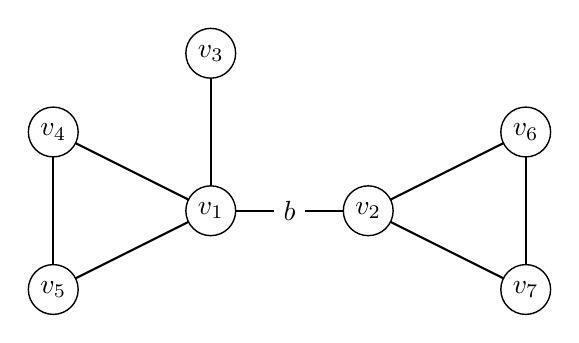
\begin{tikzpicture}
			\Vertex[x=0, y=0, L=$v_1$]{A}
			\Vertex[x=2, y=0, L=$v_2$]{B}
			\Vertex[x=0, y=2, L=$v_3$]{C}
			\Vertex[x=-2, y=1, L=$v_4$]{D}
			\Vertex[x=-2, y=-1, L=$v_5$]{E}
			\Vertex[x=4, y=1, L=$v_6$]{F}
			\Vertex[x=4,y=-1, L=$v_7$]{G}
			\Edge(D)(E)
			\Edge(D)(A)
			\Edge(E)(A)
			\Edge(A)(C)
			%\tikzstyle{LabelStyle} = [fill= white]
			\Edge[label=$b$](A)(B) 
			\Edge(B)(F)
			\Edge(B)(G)
			\Edge(F)(G)
			\end{tikzpicture}
		\end{figure}
		\begin{figure}[h!]
			\caption{The contraction of $\Gamma$ at the bridge $b$.}
			\label{fig: contraction at b}
			\centering
			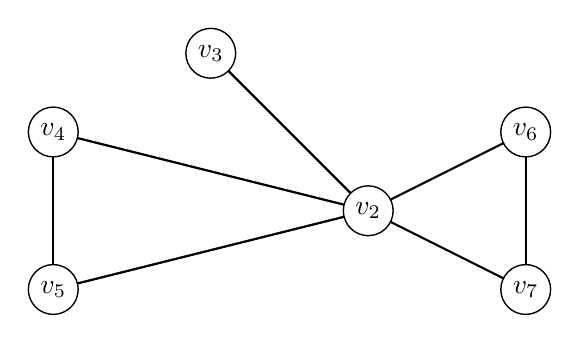
\begin{tikzpicture}
			\Vertex[x=2, y=0, L=$v_2$]{B}
			\Vertex[x=0, y=2, L=$v_3$]{C}
			\Vertex[x=-2, y=1, L=$v_4$]{D}
			\Vertex[x=-2, y=-1, L=$v_5$]{E}
			\Vertex[x=4, y=1, L=$v_6$]{F}
			\Vertex[x=4,y=-1, L=$v_7$]{G}
			\Edge(D)(E)
			\Edge(D)(B)
			\Edge(E)(B)
			\Edge(B)(C)
			%\tikzstyle{LabelStyle} = [fill= white]
			\Edge(B)(F)
			\Edge(B)(G)
			\Edge(F)(G)
			\end{tikzpicture}
		\end{figure}
		\begin{figure}[h!]
			\caption{The graph $\overline{\Gamma}$, total contraction of $\Gamma$.}
			\label{fig: total contraction}
			\centering
			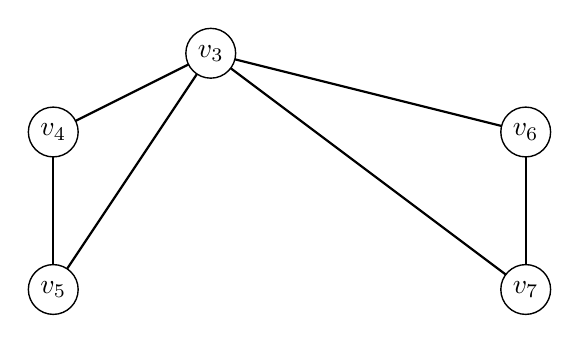
\begin{tikzpicture}
			\Vertex[x=0, y=2, L=$v_3$]{C}
			\Vertex[x=-2, y=1, L=$v_4$]{D}
			\Vertex[x=-2, y=-1, L=$v_5$]{E}
			\Vertex[x=4, y=1, L=$v_6$]{F}
			\Vertex[x=4,y=-1, L=$v_7$]{G}
			\Edge(D)(E)
			\Edge(D)(C)
			\Edge(E)(C)
			%\tikzstyle{LabelStyle} = [fill= white]
			\Edge(C)(F)
			\Edge(C)(G)
			\Edge(F)(G)
			\end{tikzpicture}
		\end{figure}
	\end{exm}
	Thus, the contraction along a bridge $b$ in practice "contracts" the bridge $b$ of a graph $\Gamma$ in such a way that the two extrema of $b$ coincide in the contraction. The total contraction consists of simply repeating this process for every bridge in $\br(\Gamma).$
	
	Following this intuitive idea, we can also see how contraction works on divisors. In particular, let $\Gamma=(V(\Gamma),E(\Gamma))$ be a graph and consider $D_\alpha= \sum_{v \in V(\Gamma)} \alpha_v v$ a divisor on $\Gamma.$ The \emph{projection} of $D_\alpha$ to $\overline{\Gamma}$ consists in a divisor $\overline{D_\alpha} = \sum_{v \in V(\overline{\Gamma})} \overline{\alpha}_v v$ such that $\overline{\alpha}_v$ is the sum of every $\alpha_w$ for each $w \in V(\Gamma)$ which was contracted to $v$  in the total contraction process.
	\begin{oss}
		Since the sum of the coefficients in $\overline{D_\alpha}$ does not differ from the sum of the coefficients in $D_\alpha$, this implies that $$\deg(\overline{D_\alpha}) = \deg(D_\alpha).$$ In particular, if $D_\alpha$ was a divisor of degree zero on $\Gamma$, then its projection $\overline{D_\alpha}$ is a divisor of degree zero on $\overline{\Gamma}.$
	\end{oss}
	\begin{oss}\label{oss: H1 bridge}
		By Lemma \ref{lem: bridge cycle}, we know that, if $b \in \br(\Gamma)$ is a bridge of a graph $\Gamma$, then $\pi(b)=0 \in H_1(\Gamma, \Z)$, because $b$ is not contained in any cycle. This implies that $$H_1(\Gamma, \Z) \simeq H_1(\overline{\Gamma},\Z).$$
	\end{oss}
	An immediate consequence of this remark is that $$b_1(\Gamma) = b_1(\overline{\Gamma}).$$
	
	\section{The Theorem and its proof}
	In this section, we sum up what we did so far and use all the tools defined previously in order to show the following Theorem, which is another original result of this thesis.
	\begin{thm}\label{thm: equality green ahp}
		Let $\F$ be $\Q$ or $\R.$ Let $(f\colon X \rightarrow \Delta^r, (x_1, \dots, x_n))$ be a $n$-pointed universal family of curves with stable degeneration over the polydisk $\Delta^r$ and suppose that on $\Delta^r$ is defined a normal crossings divisor $S := \{s_1 \cdots s_r =0\}$. Denote with $X_0$ the central fiber and let $\Gamma := \text{Graph}(X_0) =(V,E)$ be the dual graph associated to the central fiber. Since we fixed $n$ points on $X$, to give a family of divisors on $X$ it is sufficient to give a vector $\alpha =(\alpha_1, \dots, \alpha_n)\in \Z^n$, so that the associated family of divisors becomes $D_\alpha := \sum_{i=1}^n \alpha_i \cdot x_i.$ Therefore, let $\alpha, \beta \in \Z^n$ be such that $\sum_{i=1}^n \alpha_i = \sum_{i=1}^n \beta_i = 0.$ Let $\nu_\alpha, \nu_\beta\in H^0(\Delta^r, \mathcal{J}_1)$ be admissible normal functions associated respectively to $\alpha$ and $\beta$. Let $k_\alpha := k_{\nu_\alpha}, k_\beta:=k_{\nu_\beta}$ be the corresponding crossed homomorphisms in $H^1_G(\Z^r, H).$
		Let $t = (t_e \mid e \in E) \in \F^{|E|}_{\ge 0}$ be a weight function on the edges of $\Gamma$ and let $g_\Gamma(t)(D,D')$ be the weighted Green function defined in \ref{def: weighted Green function} on divisors of degree zero on $\Gamma.$ Let $h_Q(t)(\sing(\nu_\alpha),\sing(\nu_\beta))$ be the asymptotic height pairing on the singularities of $\nu_\alpha, \nu_\beta$. Then, for any $t \in \F^{|E|}_{\ge 0}$, it holds that \begin{equation}\label{eq: ahp equal Green}
		h_Q(t)(\sing(\nu_\alpha), \sing(\nu_\beta)) = g_{\overline{\Gamma}}(t)(\overline{D_\alpha}, \overline{D_\beta}),
		\end{equation} where $\overline{\Gamma} = (\overline{V},\overline{E})$ is the total contraction of $\Gamma$ and $\overline{D_\alpha}, \overline{D_\beta}$ are the projections of $D_\alpha,D_\beta$ on $\overline{\Gamma}.$
	\end{thm}
	\begin{proof}
		Let $M_t = \sum_{e \in E} t_e M_e$, where $M_e$ is the cycle pairing defined in Definition \ref{def: bilnear form Me}.	From the beginning of the proof of Theorem \ref{explicit formula}, it is enough to show that \begin{equation}\label{eq: reduction of theorem} \sum_{e \in E} t_eM_e (\psi(h_{\alpha,e}), \psi(h_{\beta,e} -l(t))) = g_{\overline{\Gamma}}(t)(\overline{D_\alpha}, \overline{D_\beta}).\end{equation} As we already observed in the proof of Theorem \ref{explicit formula}, since both sides of the equality are bi-additive in $\alpha,\beta$, we can reduce ourselves to the case where $D_\alpha = x_1 - x_2$ and $D_\beta = x_1' - x_2'.$ 
		
		Suppose now that $x_1, x_2, x_1', x_2'$ evaluated in $0$ induce (respectively) vertices $p,q,p',q'$ on $\Gamma.$ If we denote again with $D_\alpha, D_\beta$ the divisors induced on $\Gamma$, we have that $$D_\alpha = p - q, \quad D_\beta = p'-q'.$$ Let $\gamma_\alpha \subset \Gamma$ be a continuous simple path from $p$ to $q$ and let $\gamma_\beta \subset \Gamma$ be a continuous simple path from $p'$ to $q'$. Denote with $$\pi \colon C_1(\Gamma, \F) \twoheadrightarrow H_1(\Gamma,\F), \quad \pi' \colon C_1(\Gamma, \F) \twoheadrightarrow H_1(\Gamma, \F)^\bot$$ the orthogonal projections with respect to the bilinear form $M_t$. As already noticed in Remark \ref{oss: H1 bridge}, if $b \in \br(\Gamma)$ is a bridge, then $\pi(b)=0$. This implies that $M_b \equiv 0$ on $H_1(\Gamma,\F) \simeq H_1(\overline{\Gamma}, \F).$
		
		Hence, in the left side of equation \eqref{eq: reduction of theorem} it is enough to consider $e \in \overline{E}$ instead of $e \in E.$ Thanks to this observation, we can suppose that $\Gamma =(V,E)$ is a graph already totally contracted (i.e. $\Gamma = \overline{\Gamma}$). Thus we are left to show  \begin{equation}\label{eq: reduction of theorem 2}
		\sum_{e \in E} t_eM_e(\psi(h_{\alpha,e}), \psi(h_{\beta,e}-l(t))) = g_\Gamma(t)(D_\alpha, D_\beta),
		\end{equation} for $\Gamma$ a graph such that $\br(\Gamma)= \emptyset.$
		
		Recall that, by Definition \ref{def: ell tilde} and the discussion immediately above, we defined a cycle $\widetilde{c_e} \in H:= H_1(X_{b_0},\Z)$ and a path $\widetilde{\ell_e} \in H$, where $b_0 \in (\Delta^*)^r.$ In a similar way as did there, we will define $\widetilde{\ell_e'} \in H$, by $$\widetilde{\ell_e'} := \begin{cases}
		\widetilde{c_e} \quad \text{if } e \in \gamma_\alpha;\\ 0 \quad \text{if } e \notin \gamma_\alpha.
		\end{cases}$$ 
		From \eqref{eq: Ne hbetae = Ne ell e}, we obtain that $$Q(h_{\beta,e},c_e) = Q(\widetilde{\ell_e},c_e).$$ This implies that $$[\psi(h_{\alpha,e})]_e = M_e(\psi(h_{\alpha,e}),e) = Q(h_{\alpha,e},c_e) = Q(\widetilde{\ell'_e},c_e) = [\psi(\widetilde{\ell'_e})]_e.$$ Therefore, from equation \eqref{eq: reduction of theorem 2}, we have reduced to show that the following is true \begin{equation}\label{eq: reduction of theorem 3}
		\sum_{e \in E} t_e M_e(\psi(\widetilde{\ell_e'}), \psi(\widetilde{\ell_e})- \psi(l(t))) = g_\Gamma(t)(D_\alpha, D_\beta).
		\end{equation} 
		By part (2) of Lemma \ref{lem: 1}, for every $e\in E$ we have that $$[\psi(\widetilde{\ell_e})]_e = [\gamma_\beta]_e, \quad [\psi(\widetilde{\ell_e'})]_e =[\gamma_\alpha]_e.$$ Thus we obtain that $$M_e(\psi(\widetilde{\ell_e'}), \psi(\widetilde{\ell_e})-\psi(l(t))) = M_e(\gamma_\alpha, \gamma_\beta - \psi(l(t))).$$ So we further reduced ourselves to prove that 
		\begin{equation}
		M_t(\gamma_\alpha, \gamma_\beta - \psi(l(t))) = g_\Gamma(t)(D_\alpha, D_\beta).
		\end{equation}
		\begin{claim*}%\label{claim: psi(l(t))}
			$\psi(l(t)) = \pi(\gamma_\beta).$
		\end{claim*}
		\begin{proof}[Proof of Claim]
			By Lemma \ref{lem: 5} we have that $$\psi(l(t)) = \sum_{e,f \in E} t_e t_f^{-1} M_e(\psi(\widetilde{\ell_e}), \pi(f))\pi(f) = \sum_{f \in E} t_f^{-1} M_t(\gamma_\beta, \pi(f)) \pi(f).$$ On the other hand, since $\Gamma$ has only non-separating edges, we have that  $$\pi(\gamma_\beta) = \sum_{f \in E} t_f^{-1} M_t(\pi(\gamma_\beta), f) f = \sum_{f \in E} t_f^{-1} M_t(\pi(\gamma_\beta),\pi(f))\pi(f) = \sum_{f \in E} t_f^{-1} M_t(\gamma_\beta, \pi(f))\pi(f).$$
		\end{proof}
		Therefore, we have just to prove that \begin{equation}
		M_t(\gamma_\alpha, \gamma_\beta - \pi(\gamma_\beta)) = g_\Gamma(t)(D_\alpha, D_\beta).
		\end{equation}
		Since we defined $\pi' \colon C_1(\Gamma, \F) \rightarrow H_1(\Gamma, \F)^\bot$ and $\pi \colon C_1(\Gamma,\F) \rightarrow H_1(\Gamma,\F)$ to be the orthogonal projections with respect to the bilinear form $M_t,$ we get that each element $\gamma \in H_1(\Gamma, \F)$ can be written as sum of its projections, namely $\gamma = \pi(\gamma)+ \pi'(\gamma).$ In particular, we get that $$\gamma_\beta - \pi(\gamma_\beta) = \pi'(\gamma_\beta).$$ Hence we have $$M_t(\gamma_\alpha, \gamma_\beta- \pi(\gamma_\beta)) = M_t(\gamma_\alpha, \pi'(\gamma_\beta)).$$
		Now, Theorem \ref{thm: equality green ahp} follows from Proposition 7.11 of \cite{de2018metric}, which we rewrite for the ease of the reader. 
		
		Before doing so, we first introduce a bilinear form that is used in Lemma 5.2 of \cite{de2018metric}, namely the \emph{combinatorial energy pairing}. 
		\begin{defn}
			Let $\Gamma$ be a graph and let $L$ be its Laplacian matrix. Let $L^+$ be the Moore-Penrose pseudo-inverse of $L$. Then the \emph{combinatorial energy pairing}, denoted with $\langle -, - \rangle_{\text{en}}$, is defined to be the symmetric bilinear form on $\text{Div}(\Gamma)$ associated to the matrix $L^+$.
		\end{defn}
		We are now ready to state Proposition 7.11 of \cite{de2018metric}.
		\begin{lemma}
			In the same hypothesis as in Theorem \ref{thm: equality green ahp}, the following holds:
			$$\langle D_\alpha, D_\beta \rangle_{\text{en}} = M_t(\gamma_\alpha, \pi'(\gamma_\beta)).$$
		\end{lemma} 
		\begin{proof}
			See the proof of Proposition 7.11 in \cite{de2018metric}.
		\end{proof}
		Indeed, notice that $\partial \gamma_\alpha = D_\alpha$ and $\partial \gamma_\beta = D_\beta$ by definition of $\gamma_\alpha$ and $\gamma_\beta$. Moreover, we defined $g_\Gamma(-,-)$ to be represented by the Moore-Penrose pseudo-inverse of the Laplacian matrix of $\Gamma$, which is the same matrix that also represents the combinatorial energy pairing $\langle -,- \rangle_{\text{en}}$. Hence, these two bilinear forms coincide. This concludes the proof of Theorem \ref{thm: equality green ahp}.
	\end{proof}
	
	\section{Conclusion}\label{sec: conclusion}
	In Theorem \ref{thm: equality green ahp} we showed that the asymptotic height pairing of the singularities of two admissible normal functions coming from divisors of degree zero coincides with the weighted Green's function on the total contraction graph of the divisors. This is an interesting result by \emph{per se}, but it has also another nice aspect.
	Indeed, Brosnan and Pearlstein in Theorem 252 of \cite{MR3983292} prove that the asymptotic height pairing in this setting computes the \emph{height jump}, a notion introduced by Hain in \cite{MR3184171}. 
	
	On the other hand, Holmes and de Jong in the proof of Theorem 2.4 in \cite{MR3488379} prove that, in this same setting, the height jump is computed by the Green's function on the total contraction of the dual graph associated to the central fiber, namely $$j = g_{\overline{\Gamma}}(\overline{D_\alpha}, \overline{D_\beta}).$$ Hence, by Theorem \ref{thm: equality green ahp}, we showed that these two results match.
	
	We do not want to enter in the details of the height jump, because it is a wide subject beyond the target of this thesis. However, we believe that having seen how these two results, obtained using different tools, end up matching is a good conclusion of this work.

	\newpage
	\bibliographystyle{alpha}
	\addcontentsline{toc}{chapter}{References}
	\bibliography{Bibliography}
	
	
\end{document}